% Options for packages loaded elsewhere
\PassOptionsToPackage{unicode}{hyperref}
\PassOptionsToPackage{hyphens}{url}
\PassOptionsToPackage{dvipsnames,svgnames,x11names}{xcolor}
%
\documentclass[
  letterpaper,
  DIV=11,
  numbers=noendperiod,
  twocolumn,
  open=any]{scrreprt}

\usepackage{amsmath,amssymb}
\usepackage{iftex}
\ifPDFTeX
  \usepackage[T1]{fontenc}
  \usepackage[utf8]{inputenc}
  \usepackage{textcomp} % provide euro and other symbols
\else % if luatex or xetex
  \usepackage{unicode-math}
  \defaultfontfeatures{Scale=MatchLowercase}
  \defaultfontfeatures[\rmfamily]{Ligatures=TeX,Scale=1}
\fi
\usepackage{lmodern}
\ifPDFTeX\else  
    % xetex/luatex font selection
    \setmainfont[]{Arial}
\fi
% Use upquote if available, for straight quotes in verbatim environments
\IfFileExists{upquote.sty}{\usepackage{upquote}}{}
\IfFileExists{microtype.sty}{% use microtype if available
  \usepackage[]{microtype}
  \UseMicrotypeSet[protrusion]{basicmath} % disable protrusion for tt fonts
}{}
\makeatletter
\@ifundefined{KOMAClassName}{% if non-KOMA class
  \IfFileExists{parskip.sty}{%
    \usepackage{parskip}
  }{% else
    \setlength{\parindent}{0pt}
    \setlength{\parskip}{6pt plus 2pt minus 1pt}}
}{% if KOMA class
  \KOMAoptions{parskip=half}}
\makeatother
\usepackage{xcolor}
\usepackage[top=20mm,left=15mm,right=15mm,bottom=20mm,heightrounded]{geometry}
\setlength{\emergencystretch}{3em} % prevent overfull lines
\setcounter{secnumdepth}{5}
% Make \paragraph and \subparagraph free-standing
\makeatletter
\ifx\paragraph\undefined\else
  \let\oldparagraph\paragraph
  \renewcommand{\paragraph}{
    \@ifstar
      \xxxParagraphStar
      \xxxParagraphNoStar
  }
  \newcommand{\xxxParagraphStar}[1]{\oldparagraph*{#1}\mbox{}}
  \newcommand{\xxxParagraphNoStar}[1]{\oldparagraph{#1}\mbox{}}
\fi
\ifx\subparagraph\undefined\else
  \let\oldsubparagraph\subparagraph
  \renewcommand{\subparagraph}{
    \@ifstar
      \xxxSubParagraphStar
      \xxxSubParagraphNoStar
  }
  \newcommand{\xxxSubParagraphStar}[1]{\oldsubparagraph*{#1}\mbox{}}
  \newcommand{\xxxSubParagraphNoStar}[1]{\oldsubparagraph{#1}\mbox{}}
\fi
\makeatother


\providecommand{\tightlist}{%
  \setlength{\itemsep}{0pt}\setlength{\parskip}{0pt}}\usepackage{longtable,booktabs,array}
\usepackage{calc} % for calculating minipage widths
% Correct order of tables after \paragraph or \subparagraph
\usepackage{etoolbox}
\makeatletter
\patchcmd\longtable{\par}{\if@noskipsec\mbox{}\fi\par}{}{}
\makeatother
% Allow footnotes in longtable head/foot
\IfFileExists{footnotehyper.sty}{\usepackage{footnotehyper}}{\usepackage{footnote}}
\makesavenoteenv{longtable}
\usepackage{graphicx}
\makeatletter
\newsavebox\pandoc@box
\newcommand*\pandocbounded[1]{% scales image to fit in text height/width
  \sbox\pandoc@box{#1}%
  \Gscale@div\@tempa{\textheight}{\dimexpr\ht\pandoc@box+\dp\pandoc@box\relax}%
  \Gscale@div\@tempb{\linewidth}{\wd\pandoc@box}%
  \ifdim\@tempb\p@<\@tempa\p@\let\@tempa\@tempb\fi% select the smaller of both
  \ifdim\@tempa\p@<\p@\scalebox{\@tempa}{\usebox\pandoc@box}%
  \else\usebox{\pandoc@box}%
  \fi%
}
% Set default figure placement to htbp
\def\fps@figure{htbp}
\makeatother
% definitions for citeproc citations
\NewDocumentCommand\citeproctext{}{}
\NewDocumentCommand\citeproc{mm}{%
  \begingroup\def\citeproctext{#2}\cite{#1}\endgroup}
\makeatletter
 % allow citations to break across lines
 \let\@cite@ofmt\@firstofone
 % avoid brackets around text for \cite:
 \def\@biblabel#1{}
 \def\@cite#1#2{{#1\if@tempswa , #2\fi}}
\makeatother
\newlength{\cslhangindent}
\setlength{\cslhangindent}{1.5em}
\newlength{\csllabelwidth}
\setlength{\csllabelwidth}{3em}
\newenvironment{CSLReferences}[2] % #1 hanging-indent, #2 entry-spacing
 {\begin{list}{}{%
  \setlength{\itemindent}{0pt}
  \setlength{\leftmargin}{0pt}
  \setlength{\parsep}{0pt}
  % turn on hanging indent if param 1 is 1
  \ifodd #1
   \setlength{\leftmargin}{\cslhangindent}
   \setlength{\itemindent}{-1\cslhangindent}
  \fi
  % set entry spacing
  \setlength{\itemsep}{#2\baselineskip}}}
 {\end{list}}
\usepackage{calc}
\newcommand{\CSLBlock}[1]{\hfill\break\parbox[t]{\linewidth}{\strut\ignorespaces#1\strut}}
\newcommand{\CSLLeftMargin}[1]{\parbox[t]{\csllabelwidth}{\strut#1\strut}}
\newcommand{\CSLRightInline}[1]{\parbox[t]{\linewidth - \csllabelwidth}{\strut#1\strut}}
\newcommand{\CSLIndent}[1]{\hspace{\cslhangindent}#1}

\usepackage{booktabs}
\usepackage{longtable}
\usepackage{array}
\usepackage{multirow}
\usepackage{wrapfig}
\usepackage{float}
\usepackage{colortbl}
\usepackage{pdflscape}
\usepackage{tabu}
\usepackage{threeparttable}
\usepackage{threeparttablex}
\usepackage[normalem]{ulem}
\usepackage{makecell}
\usepackage{xcolor}
\KOMAoption{captions}{tableheading}
\counterwithout{figure}{chapter}
\counterwithout{table}{chapter}
\makeatletter
\renewcommand\chapter{\@startsection{chapter}{0}{\z@}%
  {-3.5ex \@plus -1ex \@minus -.2ex}%
  {2.3ex \@plus.2ex}%
  {\normalfont\Large\bfseries}}
\makeatother
text: |
  \usepackage[font={small, rm}]{caption}
\makeatletter
\@ifpackageloaded{caption}{}{\usepackage{caption}}
\AtBeginDocument{%
\ifdefined\contentsname
  \renewcommand*\contentsname{Table of contents}
\else
  \newcommand\contentsname{Table of contents}
\fi
\ifdefined\listfigurename
  \renewcommand*\listfigurename{List of Figures}
\else
  \newcommand\listfigurename{List of Figures}
\fi
\ifdefined\listtablename
  \renewcommand*\listtablename{List of Tables}
\else
  \newcommand\listtablename{List of Tables}
\fi
\ifdefined\figurename
  \renewcommand*\figurename{Figure}
\else
  \newcommand\figurename{Figure}
\fi
\ifdefined\tablename
  \renewcommand*\tablename{Table}
\else
  \newcommand\tablename{Table}
\fi
}
\@ifpackageloaded{float}{}{\usepackage{float}}
\floatstyle{ruled}
\@ifundefined{c@chapter}{\newfloat{codelisting}{h}{lop}}{\newfloat{codelisting}{h}{lop}[chapter]}
\floatname{codelisting}{Listing}
\newcommand*\listoflistings{\listof{codelisting}{List of Listings}}
\makeatother
\makeatletter
\makeatother
\makeatletter
\@ifpackageloaded{caption}{}{\usepackage{caption}}
\@ifpackageloaded{subcaption}{}{\usepackage{subcaption}}
\makeatother

\ifLuaTeX
\usepackage[bidi=basic]{babel}
\else
\usepackage[bidi=default]{babel}
\fi
\babelprovide[main,import]{english}
\ifPDFTeX
\else
\babelfont{rm}[]{Arial}
\fi
% get rid of language-specific shorthands (see #6817):
\let\LanguageShortHands\languageshorthands
\def\languageshorthands#1{}
\ifLuaTeX
  \usepackage[english]{selnolig} % disable illegal ligatures
\fi
\usepackage{bookmark}

\IfFileExists{xurl.sty}{\usepackage{xurl}}{} % add URL line breaks if available
\urlstyle{same} % disable monospaced font for URLs
\hypersetup{
  pdftitle={Hunting Effect on Individual Deer Stress Level},
  pdfauthor={Nikolai German, Thomas Witzani, Ziqi Xu, Zhengchen Yuan, Baisu Zhou},
  pdflang={en},
  colorlinks=true,
  linkcolor={blue},
  filecolor={Maroon},
  citecolor={Blue},
  urlcolor={Blue},
  pdfcreator={LaTeX via pandoc}}


\title{Hunting Effect on Individual Deer Stress Level}
\usepackage{etoolbox}
\makeatletter
\providecommand{\subtitle}[1]{% add subtitle to \maketitle
  \apptocmd{\@title}{\par {\large #1 \par}}{}{}
}
\makeatother
\subtitle{P15.2 Fortgeschrittenes Praxisprojekt}
\author{Nikolai German, Thomas Witzani, Ziqi Xu, Zhengchen Yuan, Baisu
Zhou}
\date{}

\begin{document}
\maketitle

\renewcommand*\contentsname{Table of contents}
{
\hypersetup{linkcolor=}
\setcounter{tocdepth}{2}
\tableofcontents
}

\chapter*{Abstract}
\addcontentsline{toc}{chapter}{Abstract}

Hunting activity has an impact on animal populations through removal of
individuals. Moreover, it may have a non-lethal effect of inducing
stress. In this project, we analyze the short-term stress response of
red deer in the Bavarian Forest National Park to hunting events. The
stress level of a deer was measured by the concentration of \emph{faecal
cortisl metabolites (FCMs)} in faecal samples. Combining spatiotemporal
information about the faecal samples, the deer which produced them, and
the hunting events occurred in the time period of sample collection, we
aim to address how the FCM level in a deer's faecal matter is associated
with the temporal and spatial distance to a hunting event that could
have affected the deer.

\chapter{Introduction}\label{introduction}

\section{Background}\label{background}

Apart from the change in populations size, the effects of hunting on
wildlife have so far been studied mainly on the basis of behavioral
changes. This project aims to investigate the physiological stress
response in red deer using a non-invasive method, the measurement of
FCMs.

\section{Data Generating Process}\label{data-generating-process}

The data for the project origins in the \emph{Bavarian Forest National
Park}. Its location is highlighted in green in
Figure~\ref{fig-park_location}. Within and on the borders of this area,
red deer roam freely. Some of these deer have been collared with a
GPS-device, which helps to track the movement. At some time, a
\emph{hunting event} happens and the deer experiences some amount of
stress. Later, the deer defecates (``\emph{defecation event}'').
Subsequently, researchers visit the defecation location and collect a
\emph{faecal sample}.

\begin{figure}

\centering{

\pandocbounded{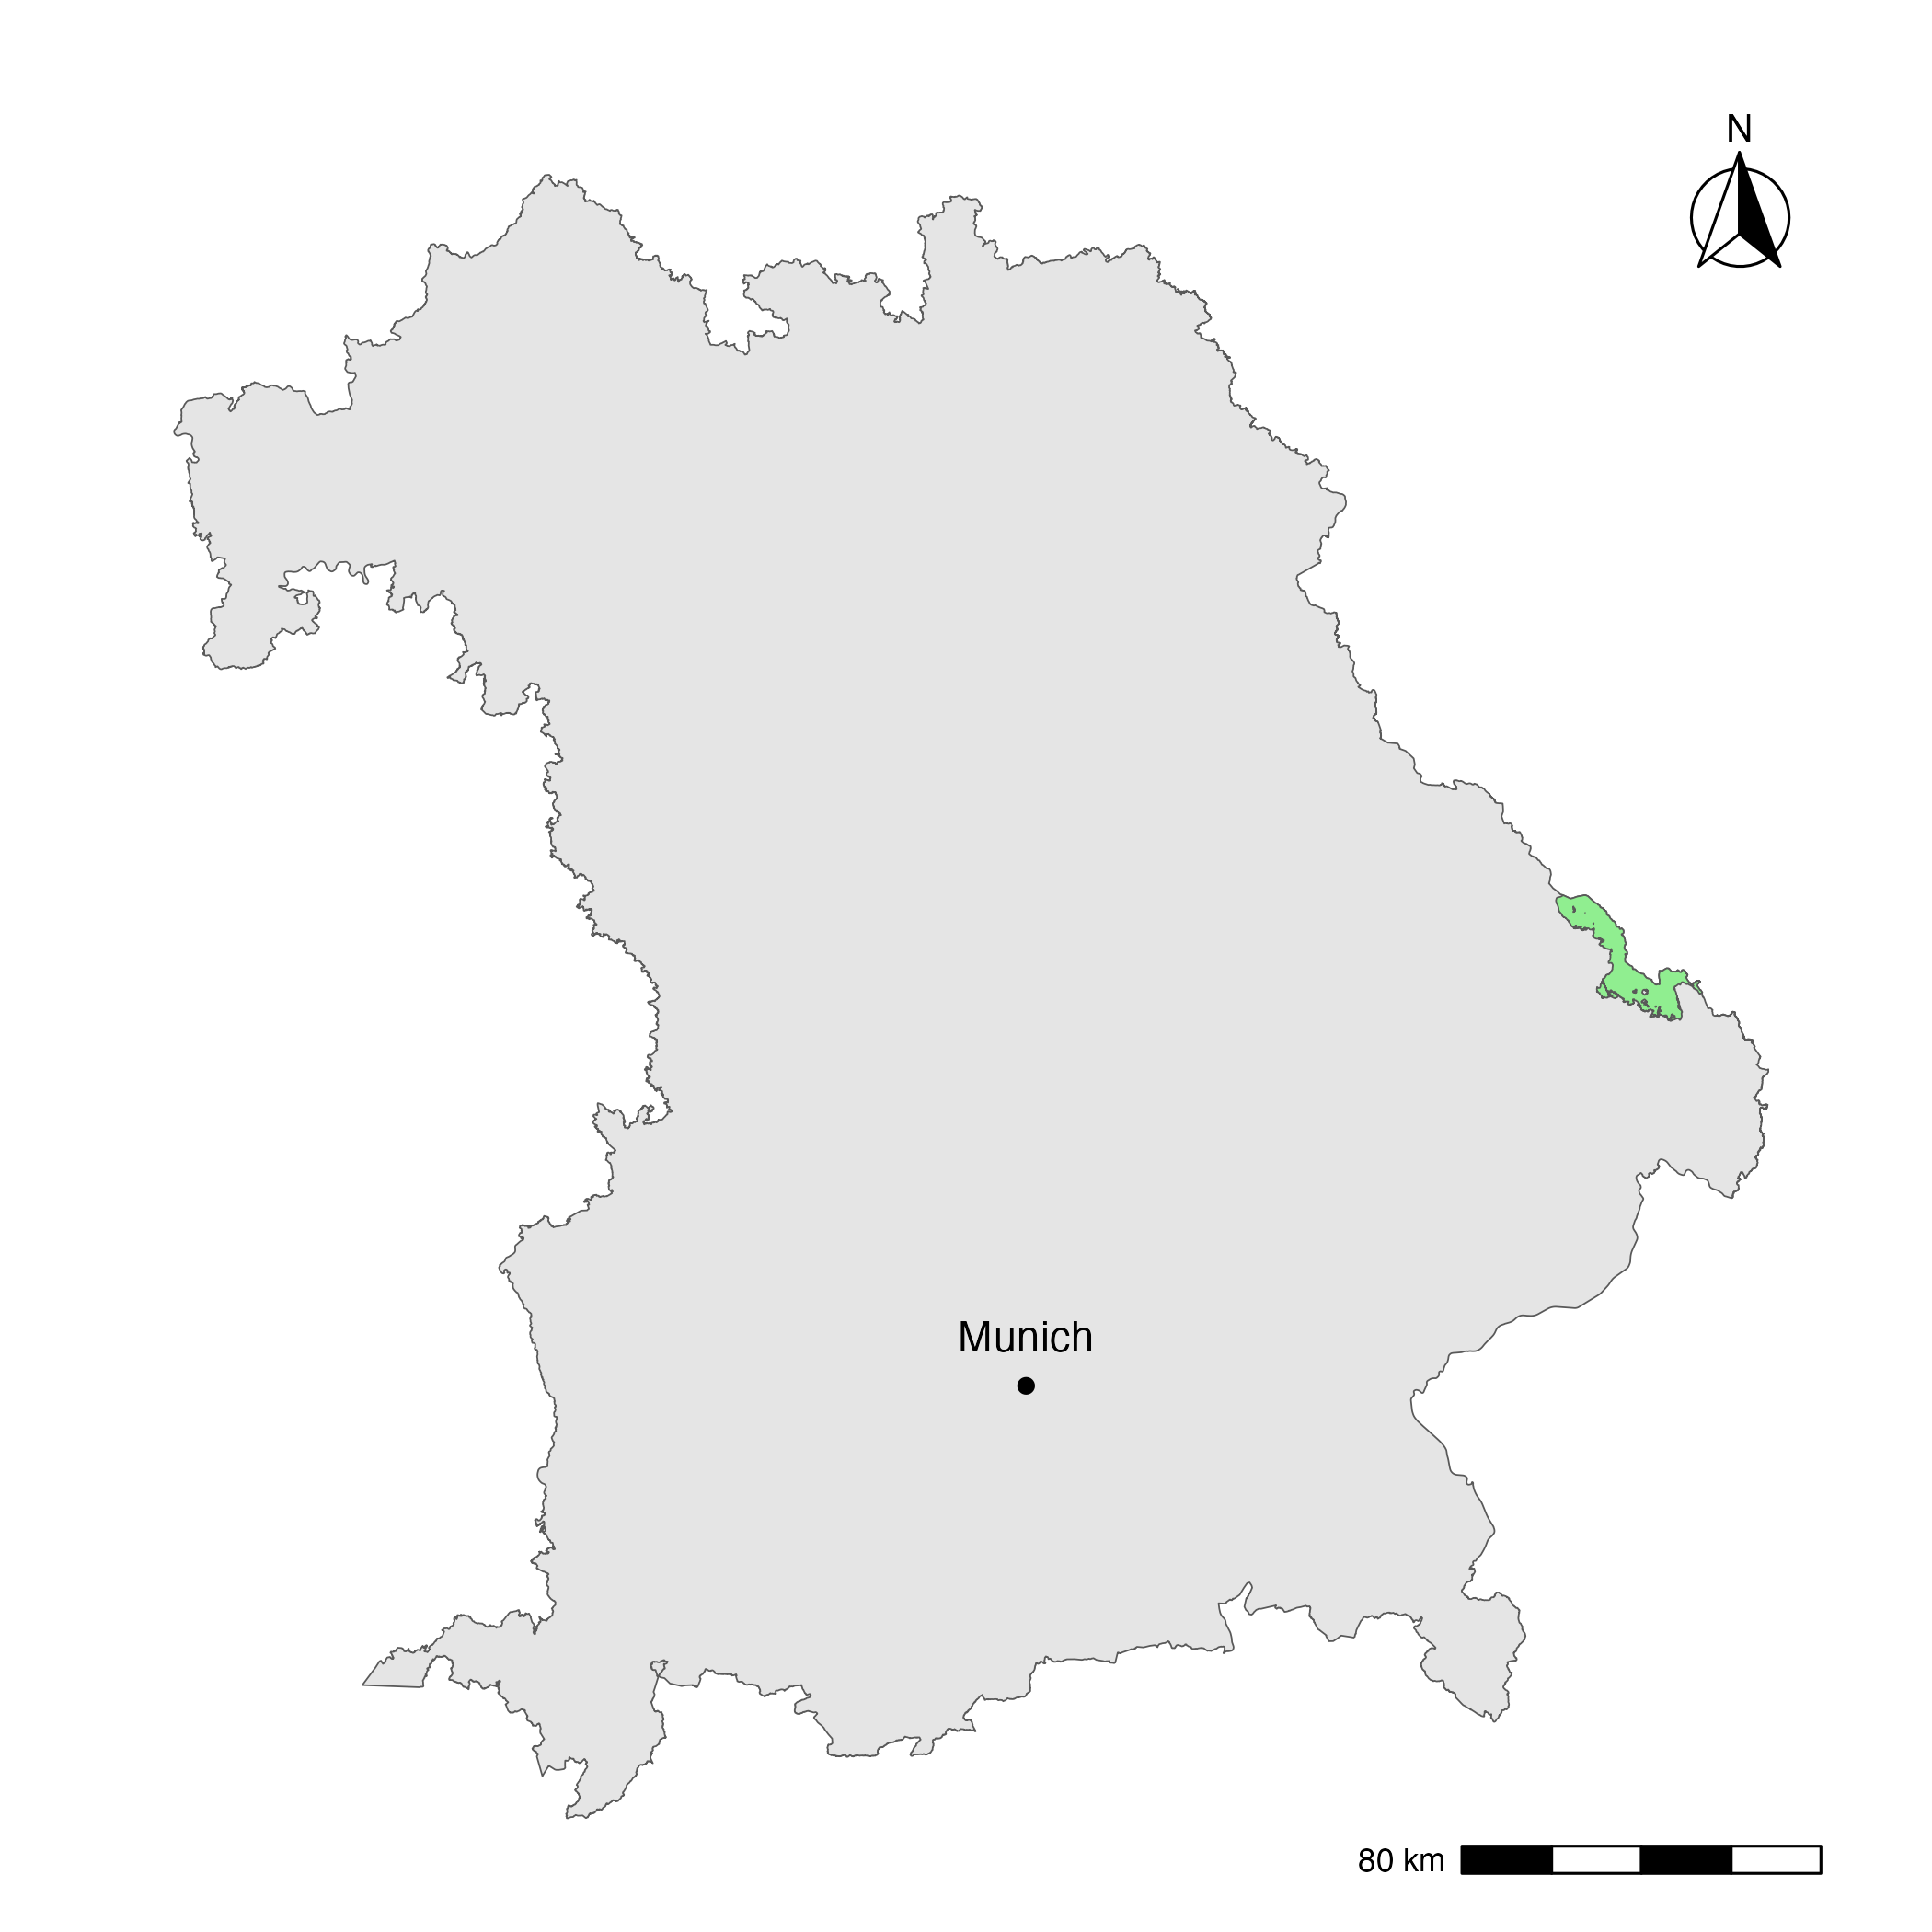
\includegraphics[keepaspectratio]{Figures/sp_park_location.png}}

}

\caption{\label{fig-park_location}Location of Bavarian Forest National
Park}

\end{figure}%

Stress is expected to be higher in proximity\footnote{Not all values
  between 1 and 365 were observed. As shown in
  Figure~\ref{fig-samples_daily_count}, faecal samples were not
  collected during winter.} to hunting events. With higher stress, FCM
values are expected to be higher. Huber et al. (2003) showed
(Figure~\ref{fig-fcm}) that the FCM levels peak between 16 and 19 hours
after a stress event (called ``challenge''). Additionally we expect,
that FCM levels are lower, the more time passes between defecation and
sampling.

\begin{figure}

\centering{

\pandocbounded{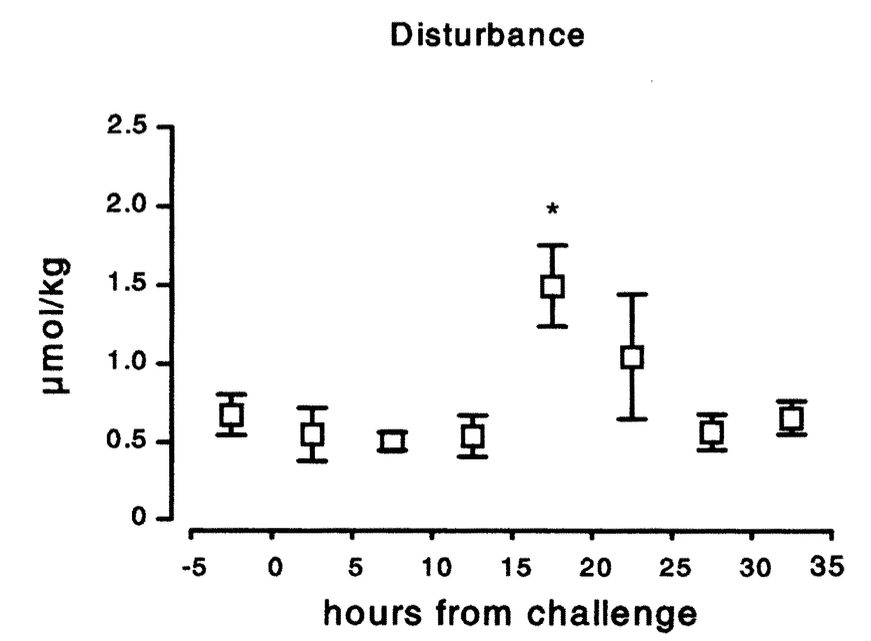
\includegraphics[keepaspectratio]{Figures/Huber_et_al_FCM_levels.png}}

}

\caption{\label{fig-fcm}FCM levels over time}

\end{figure}%

\section{Research Question}\label{research-question}

Therefore our research question is two-fold:

\begin{itemize}
\tightlist
\item
  assess the effect of temporal and spatial distance on FCM level
\item
  assess if the time between defecation event and sample collection
  affect the FCM levels
\end{itemize}

\chapter{Data Analysis}\label{data-analysis}

We were provided with four distinct datasets.~ In the following
subchapters we are going to describe the main features of each data set
and address any anomalies.

\section{Hunting Events}\label{hunting-events}

The dataset contains the location and time of 697 individual hunting
events, spanning from 2020 to 2022. There are three main challenges:

\begin{enumerate}
\def\labelenumi{\roman{enumi})}
\tightlist
\item
  Just 519 of these 697 events have a complete timestamp, consisting of
  date and time of day. The remainder of 178 events only reported the
  date of the event.
\item
  The events are not represented as a period of time, but as a as a
  single moment in time. Additionally, as shown in
  Figure~\ref{fig-hunts_dates}, there appears to be seasonality in the
  occurrence of hunts.
\item
  Similiarly to ii), the events are only associated with a single
  spatial point. The locations of the events with complete timestamps
  are illustrated in Figure~\ref{fig-hunt_locations}.
\end{enumerate}

\begin{figure}

\centering{

\pandocbounded{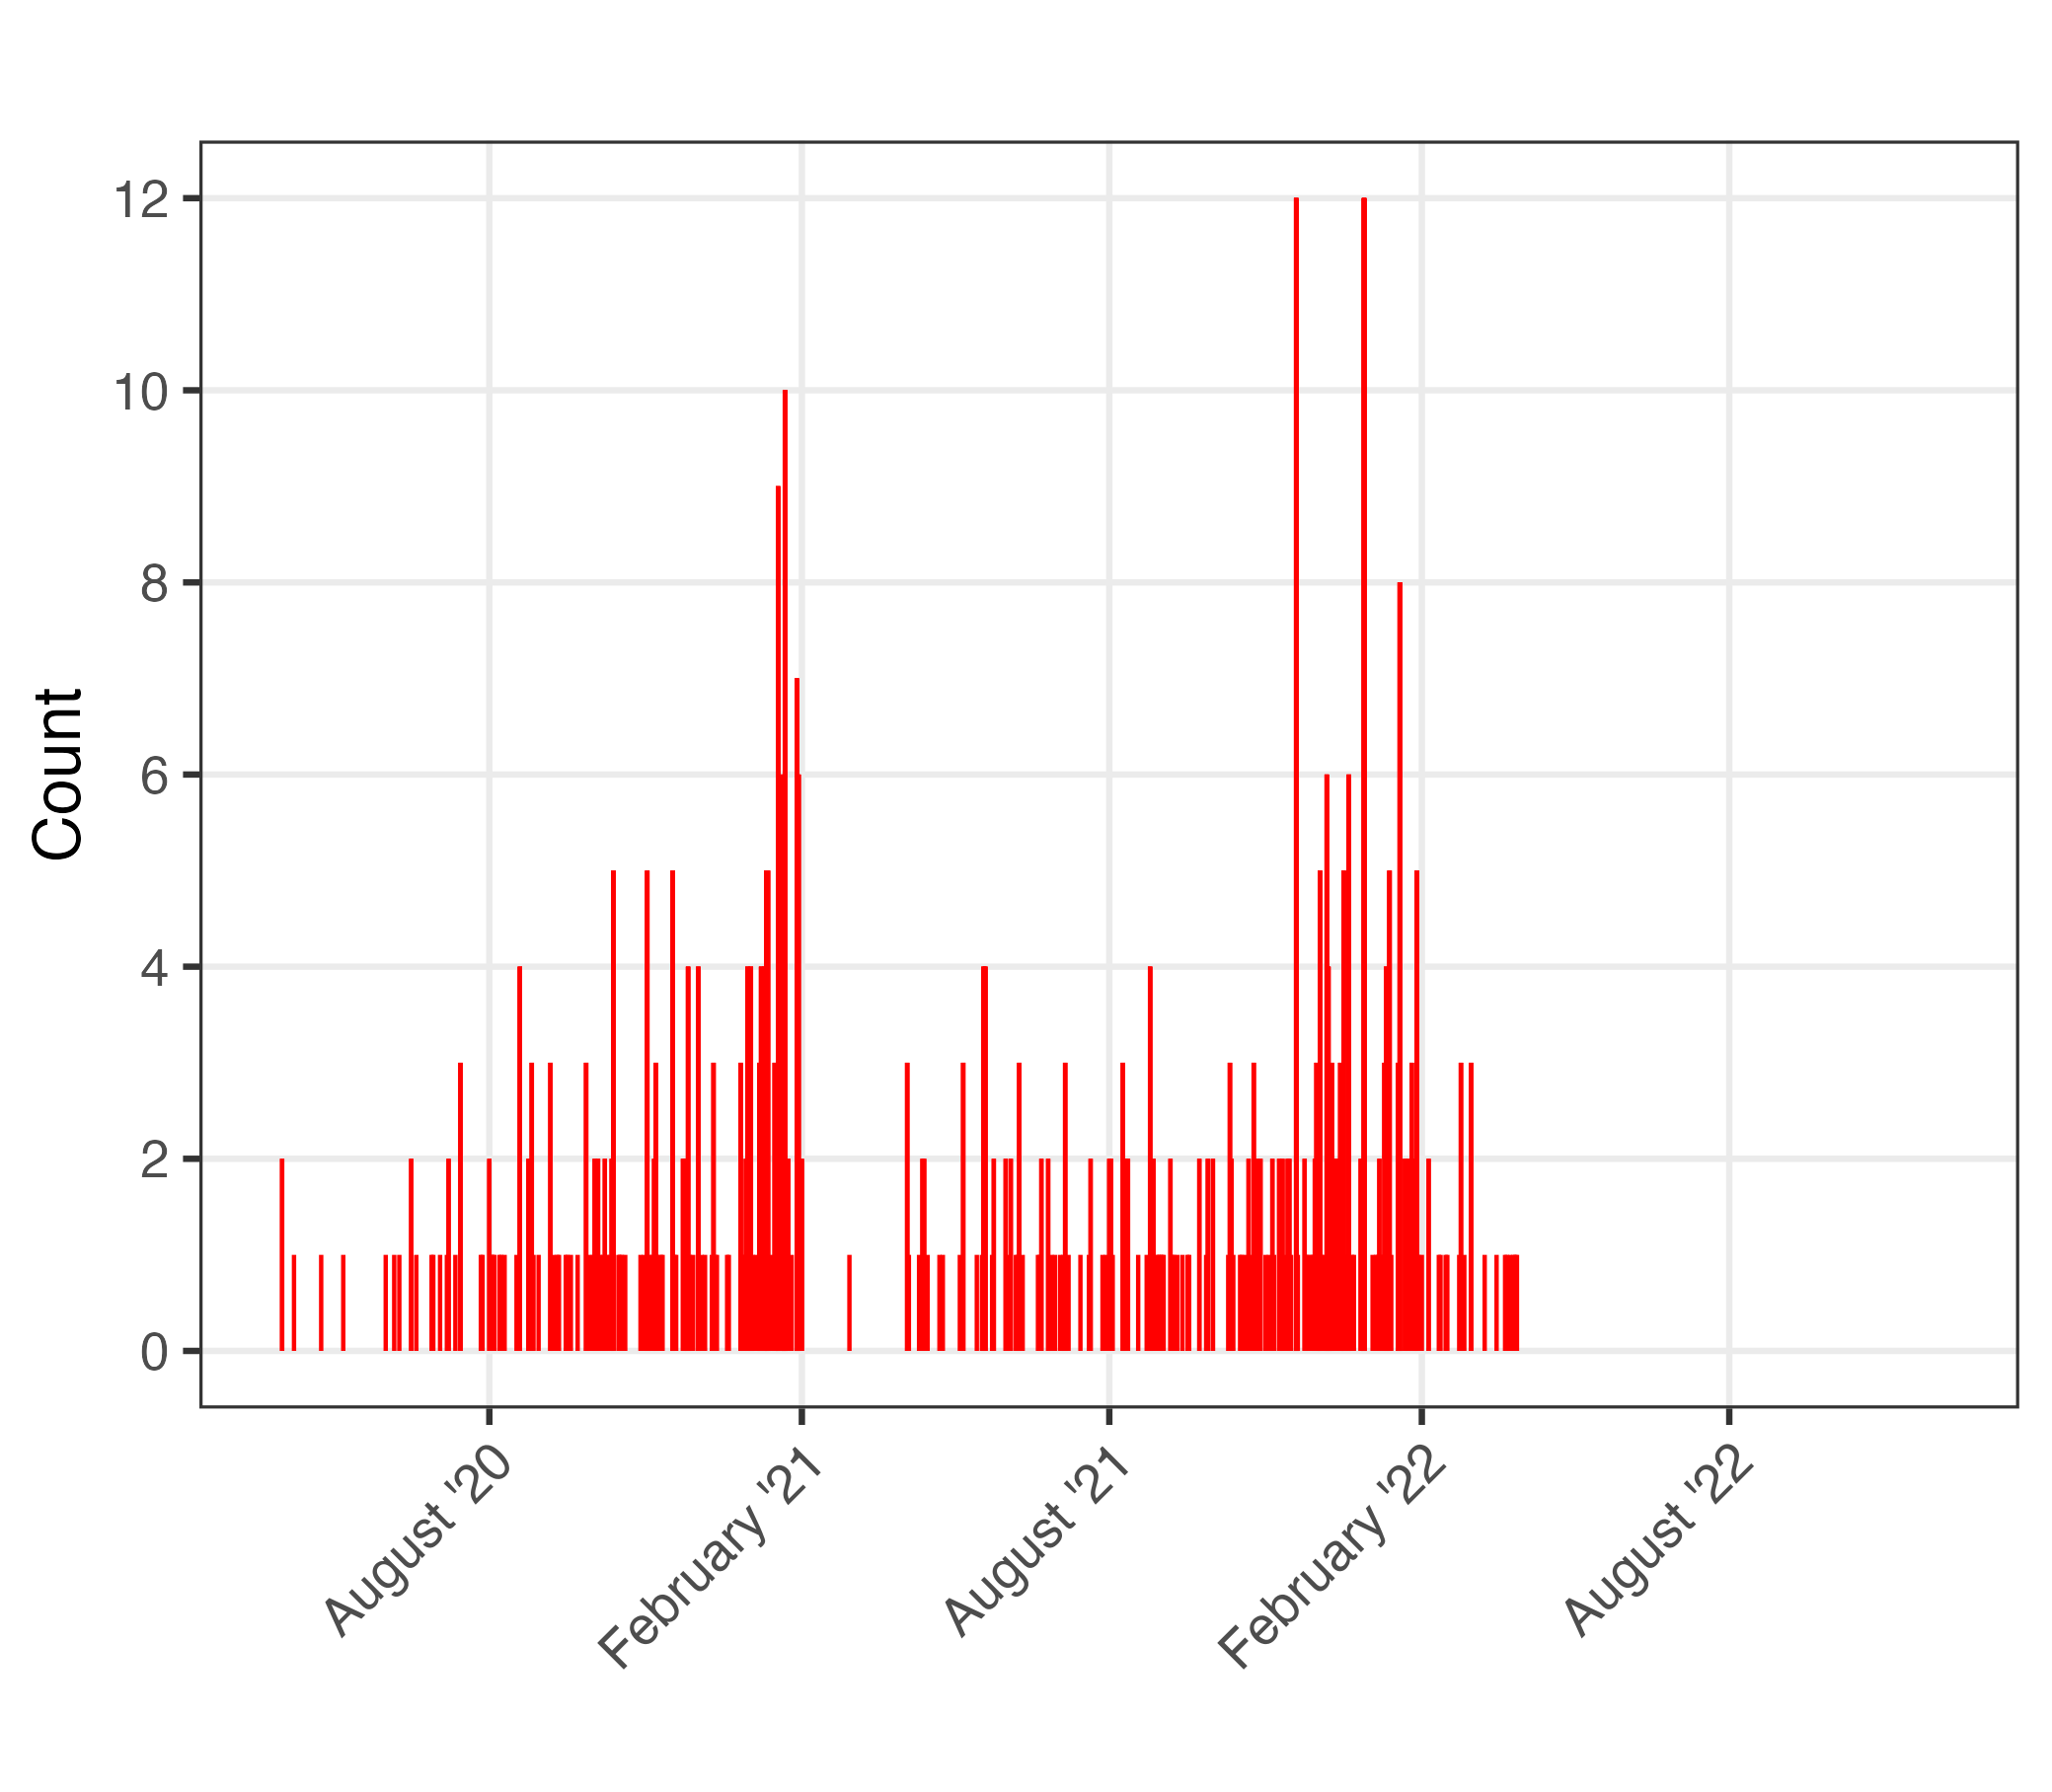
\includegraphics[keepaspectratio]{Figures/hunts_dates.png}}

}

\caption{\label{fig-hunts_dates}Hunts - Daily Count}

\end{figure}%

\begin{figure}

\centering{

\pandocbounded{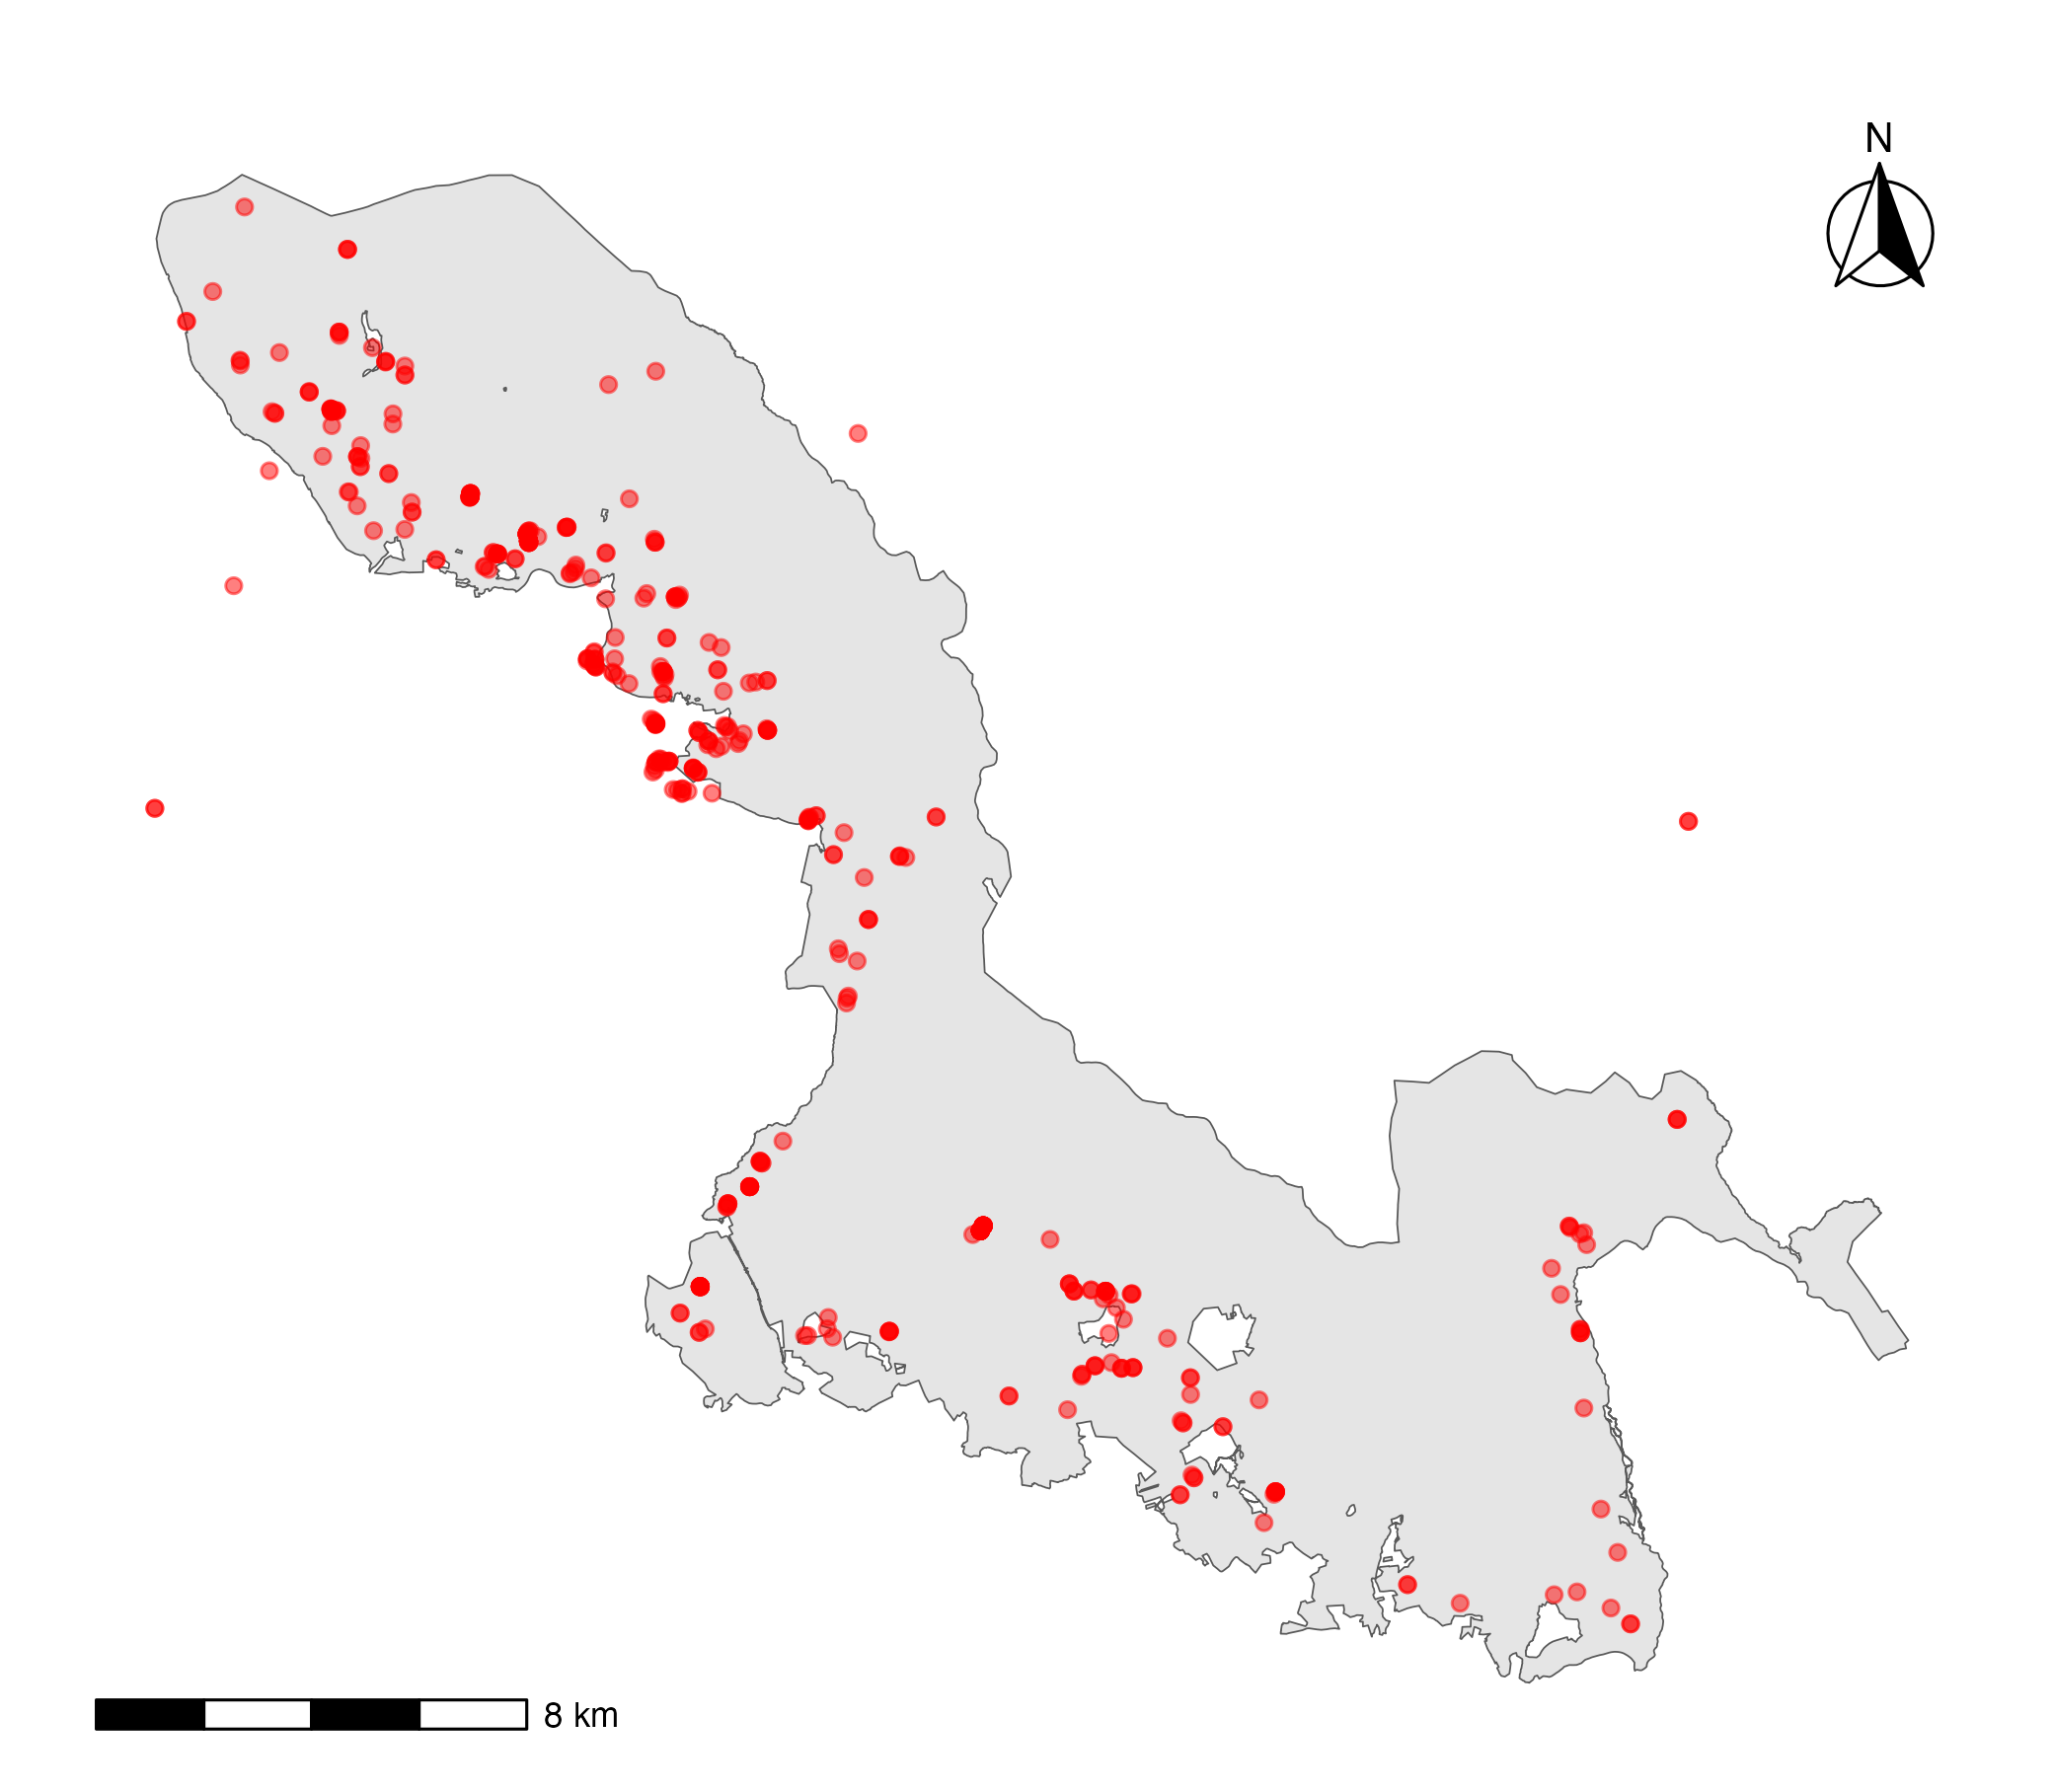
\includegraphics[keepaspectratio]{Figures/sp_hunts.png}}

}

\caption{\label{fig-hunt_locations}Hunts - Locations}

\end{figure}%

\section{Movement Data}\label{movement-data}

There are 40 collared deers which movements have been tracked completely
or partially between February 2020 and February 2023. Some collars
stopped working before the end-date, some deers got collared within the
timespan of interest. The location of each individual deer is tracked on
an hourly basis. The movement of four randomly selected deer is
visualised in Figure~\ref{fig-deers_locations}. During the winter
months, the deers roam in one of four enclosures within the national
park.

\begin{figure}

\centering{

\pandocbounded{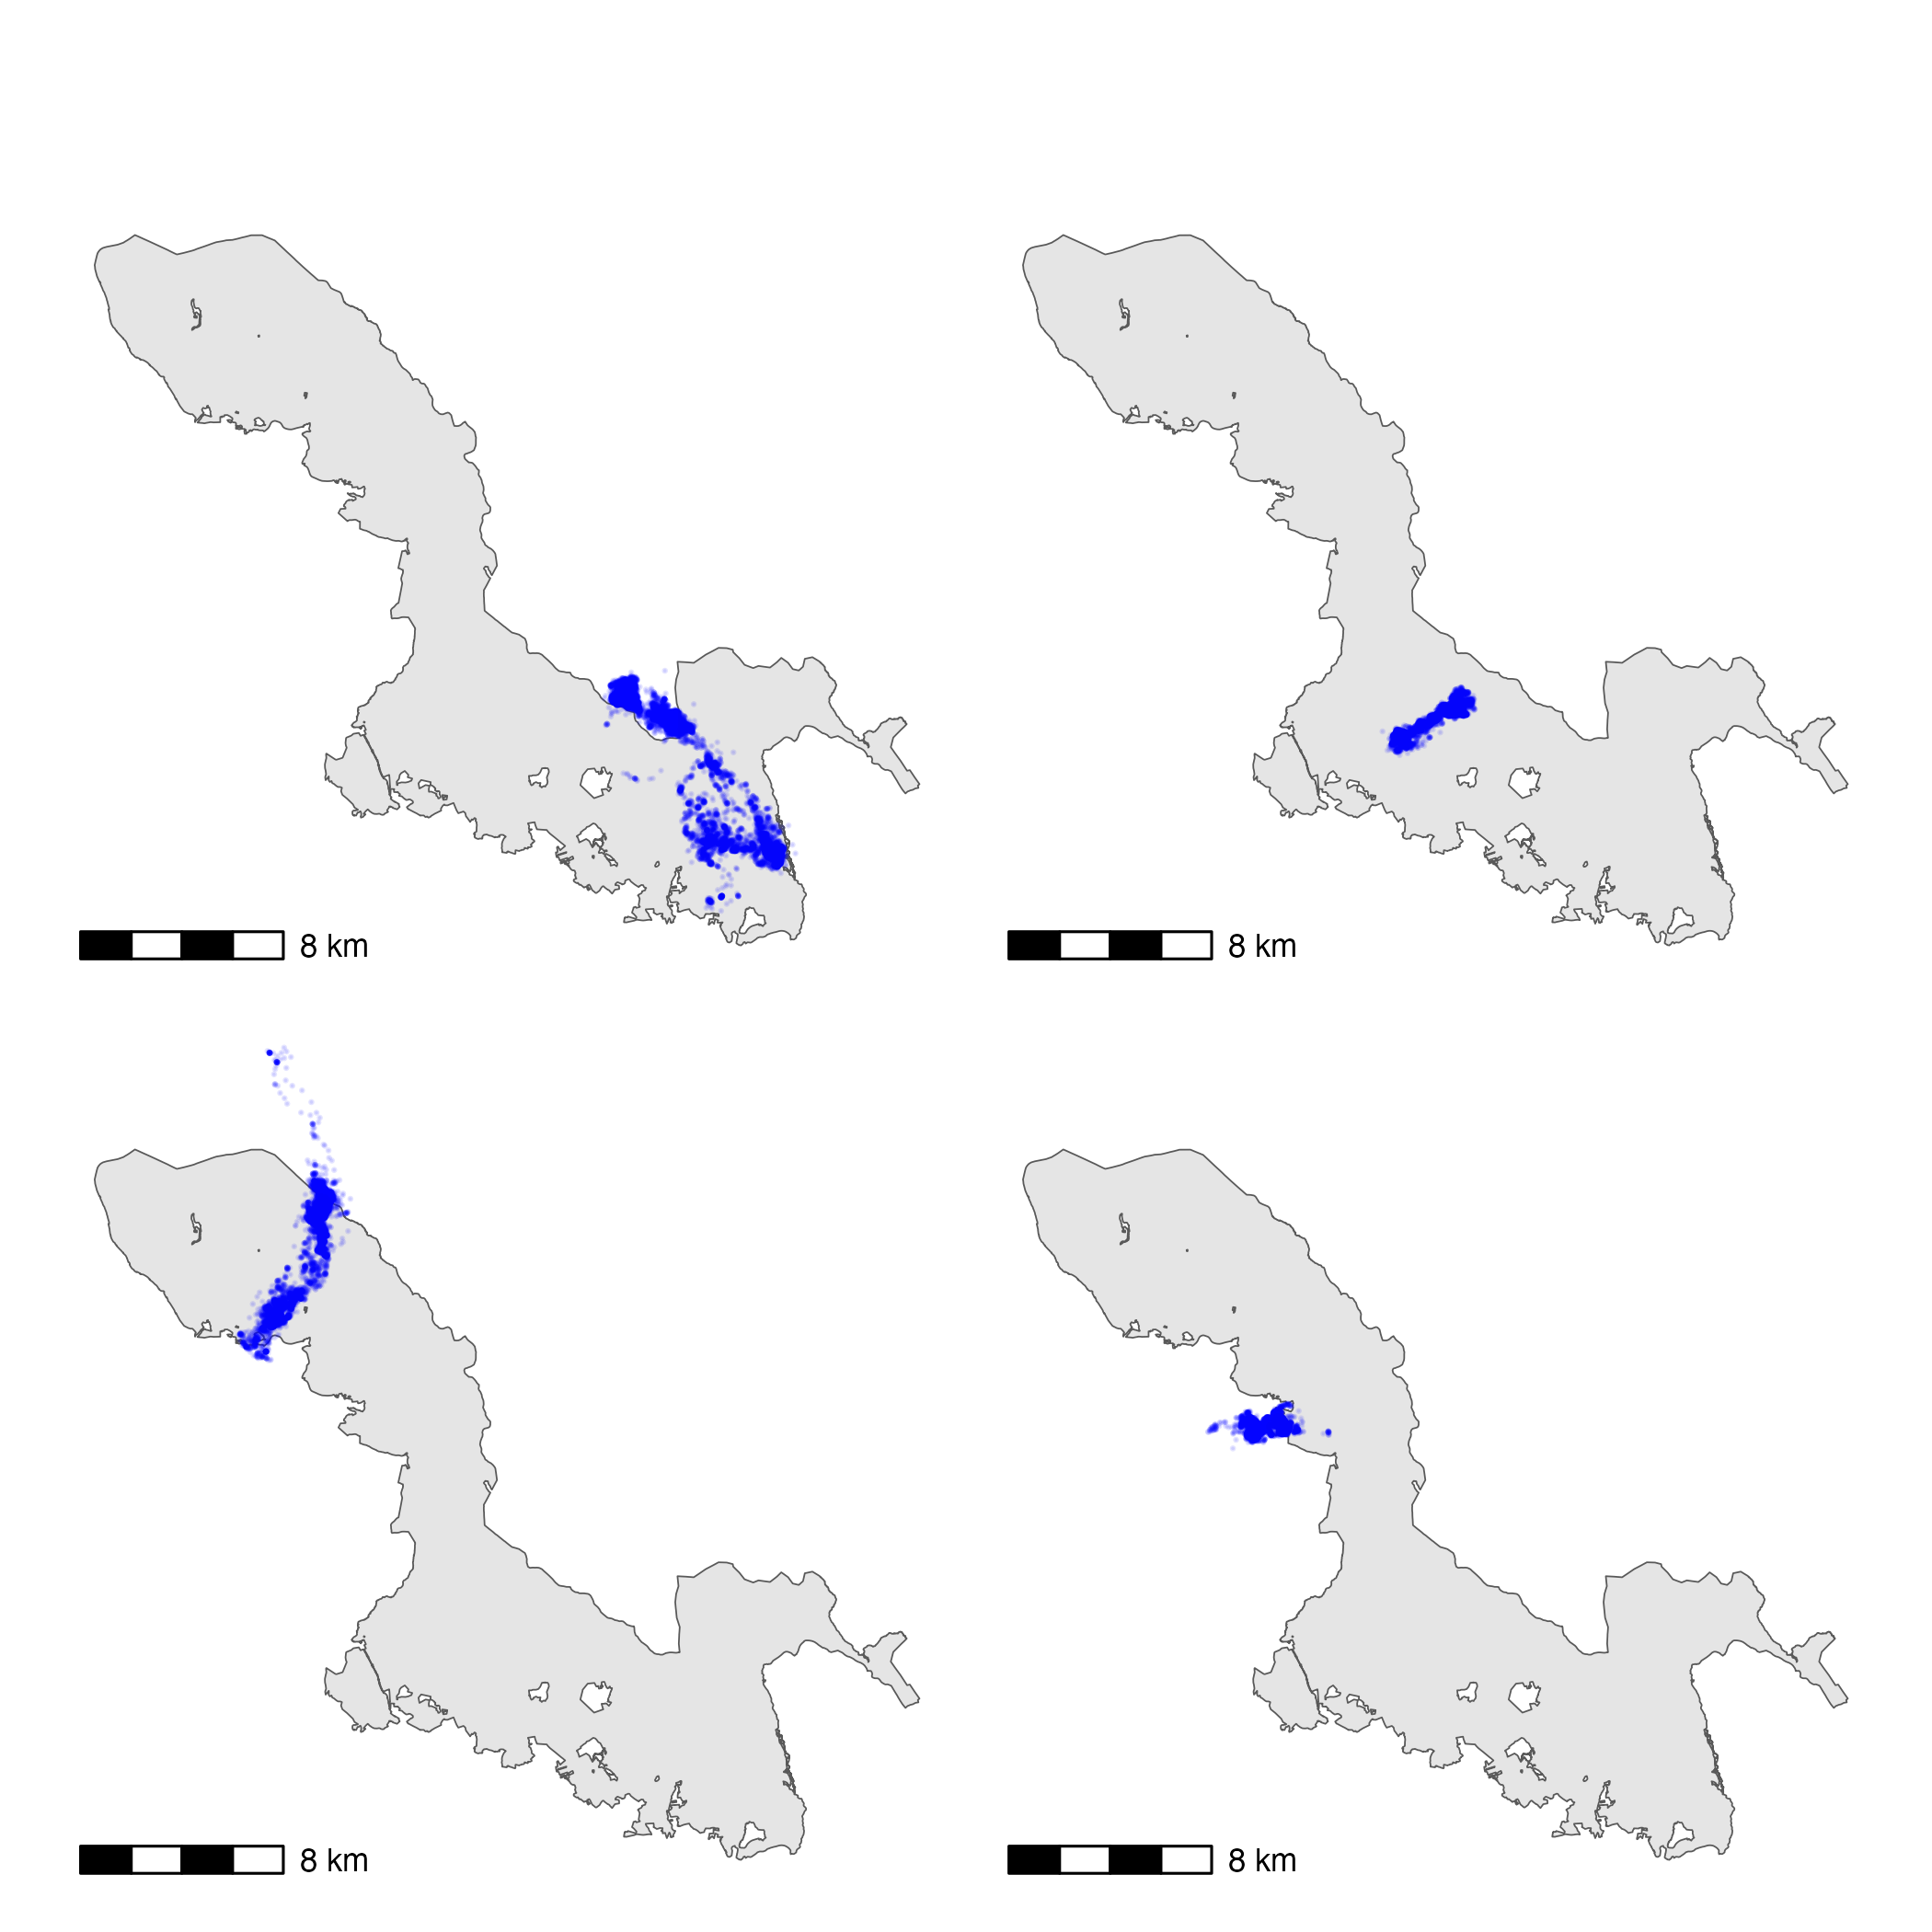
\includegraphics[keepaspectratio]{Figures/sp_movement_4.png}}

}

\caption{\label{fig-deers_locations}Deers - Locations of four Deer}

\end{figure}%

\section{Faecal Sample Data}\label{faecal-sample-data}

The faecal sample dataset contains information on 809 faecal samples.
Most importantly, the FCM level (in nanograms per gram {[}ng/g{]}), the
location of the sample, as shown in Figure~\ref{fig-samples_locations},
the associated collared deer, the approximate time of defecation and the
time of sampling. The samples were taken at irregular intervals, but
with obvious seasonality (see Figure~\ref{fig-samples_daily_count}) from
2020 to 2022.

\begin{figure}

\centering{

\pandocbounded{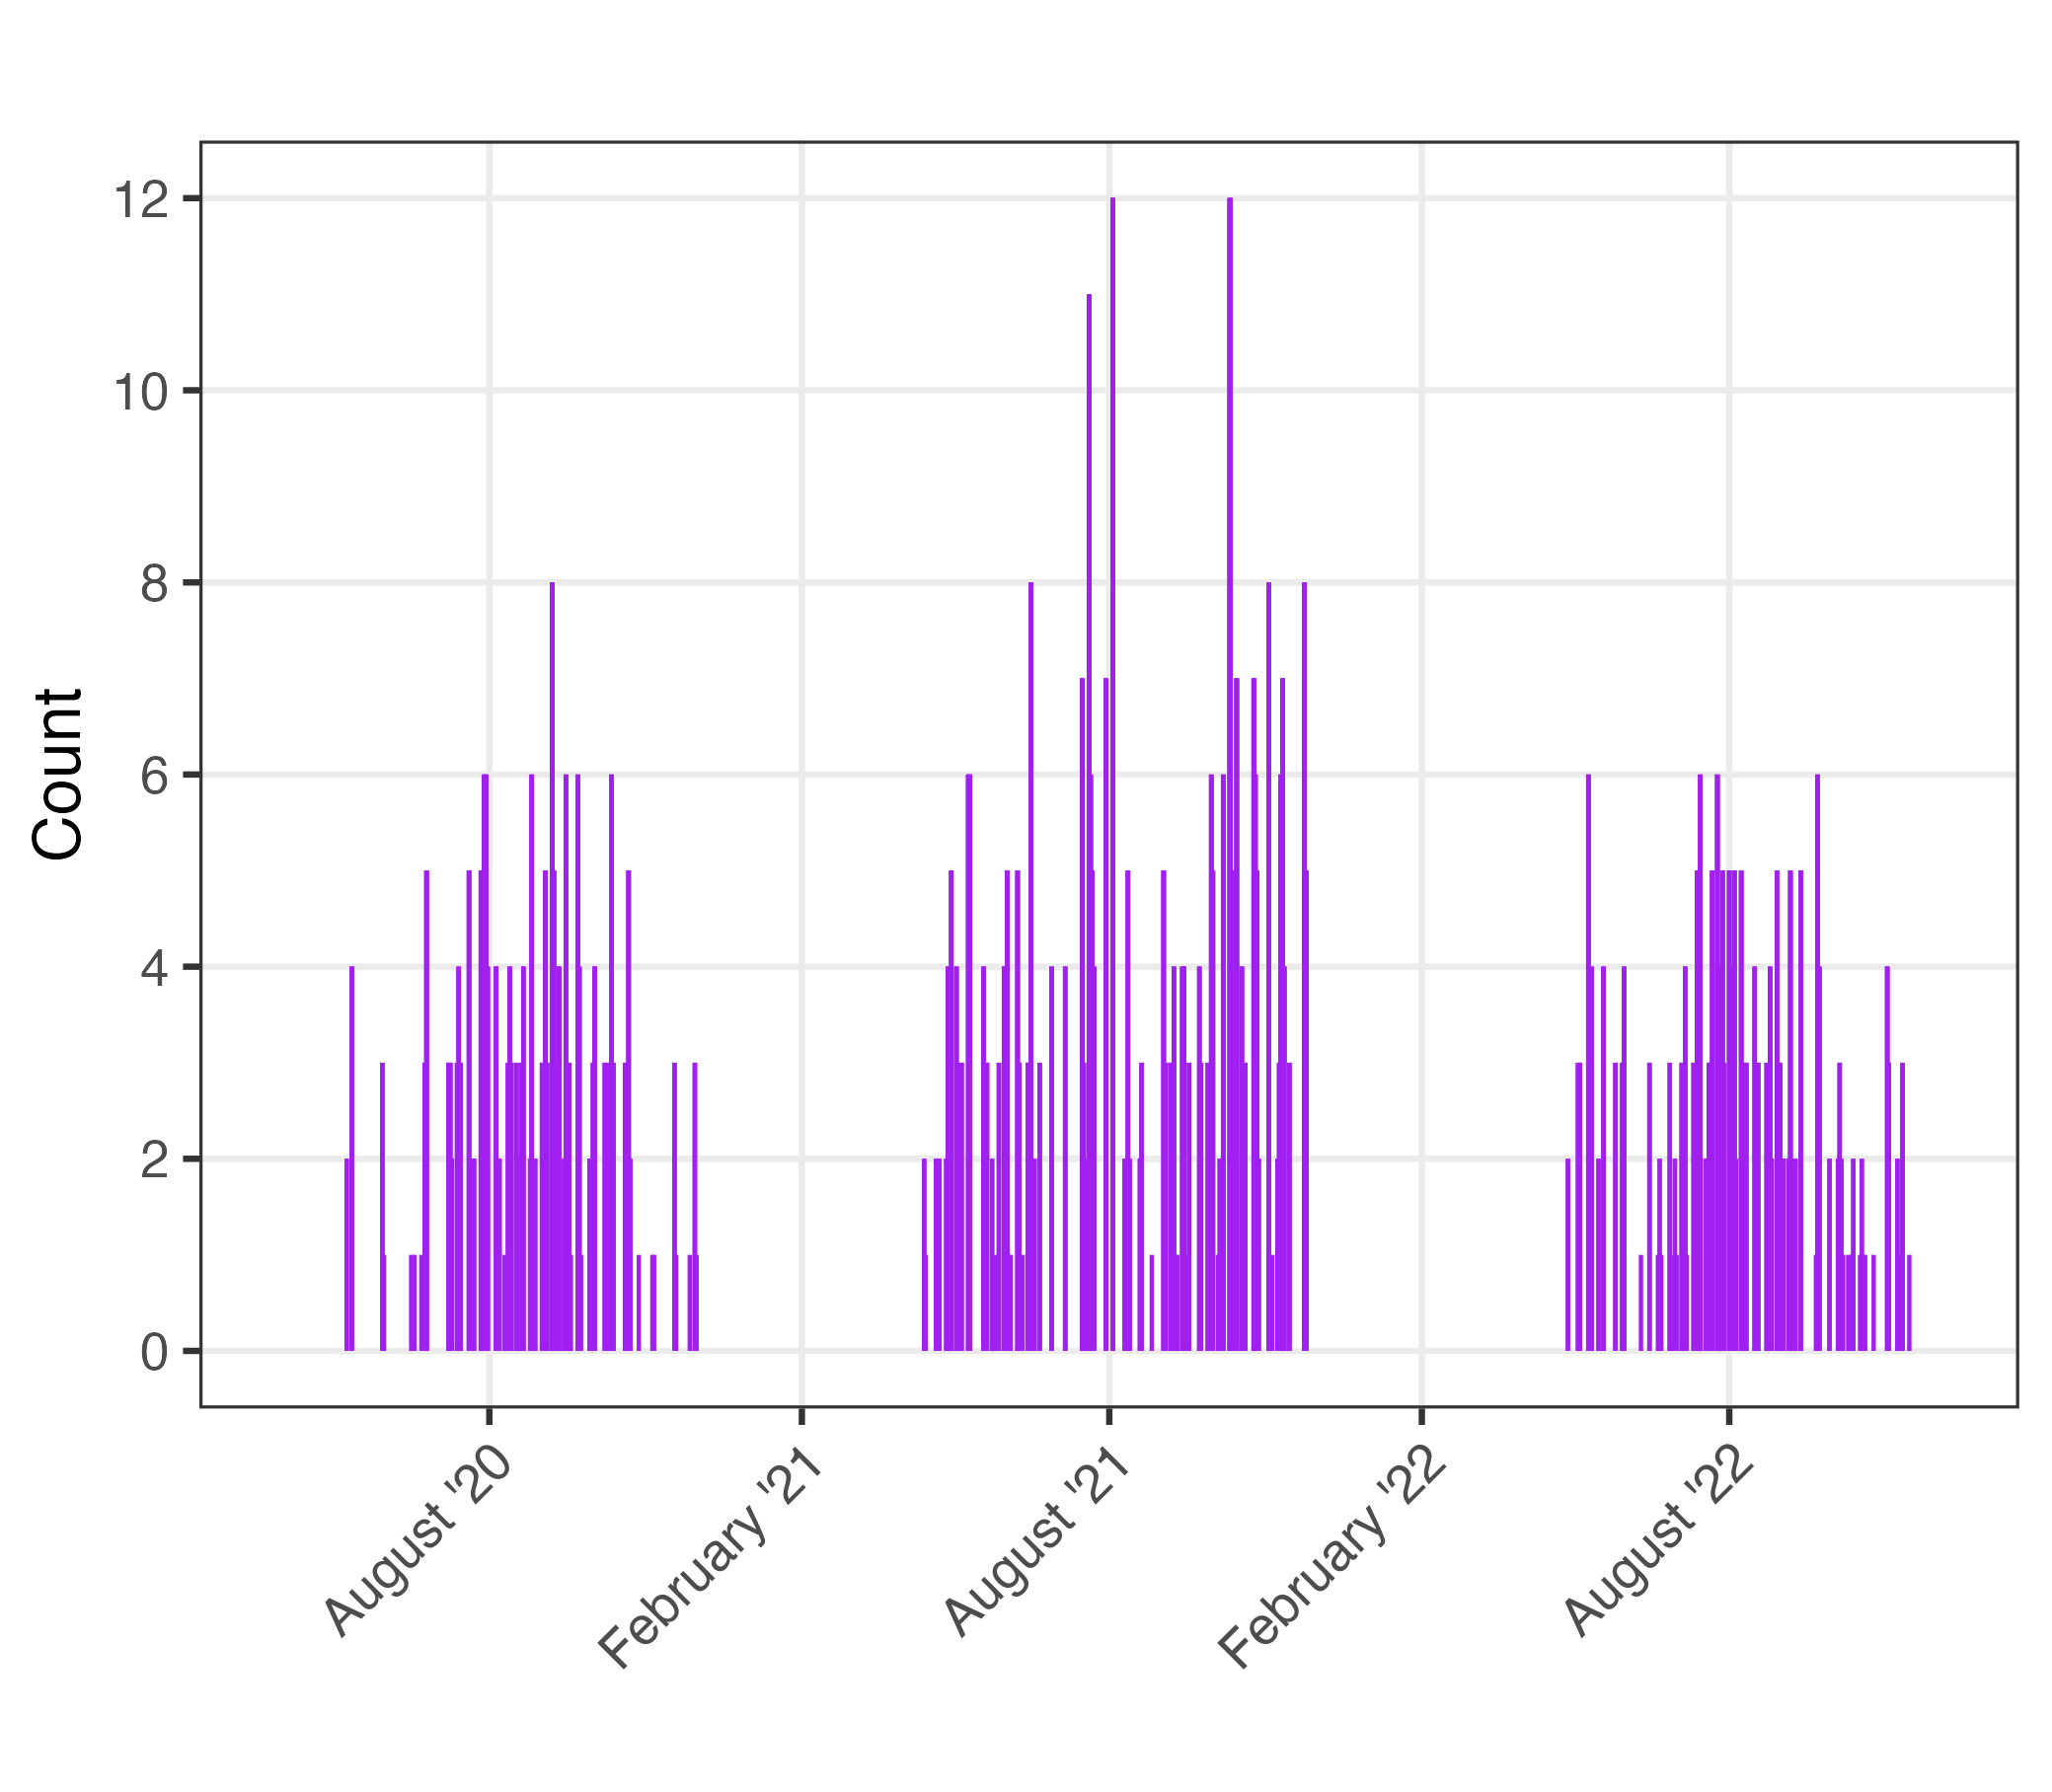
\includegraphics[keepaspectratio]{Figures/samples_daily_count.png}}

}

\caption{\label{fig-samples_daily_count}Samples - Daily Count}

\end{figure}%

\begin{figure}

\centering{

\pandocbounded{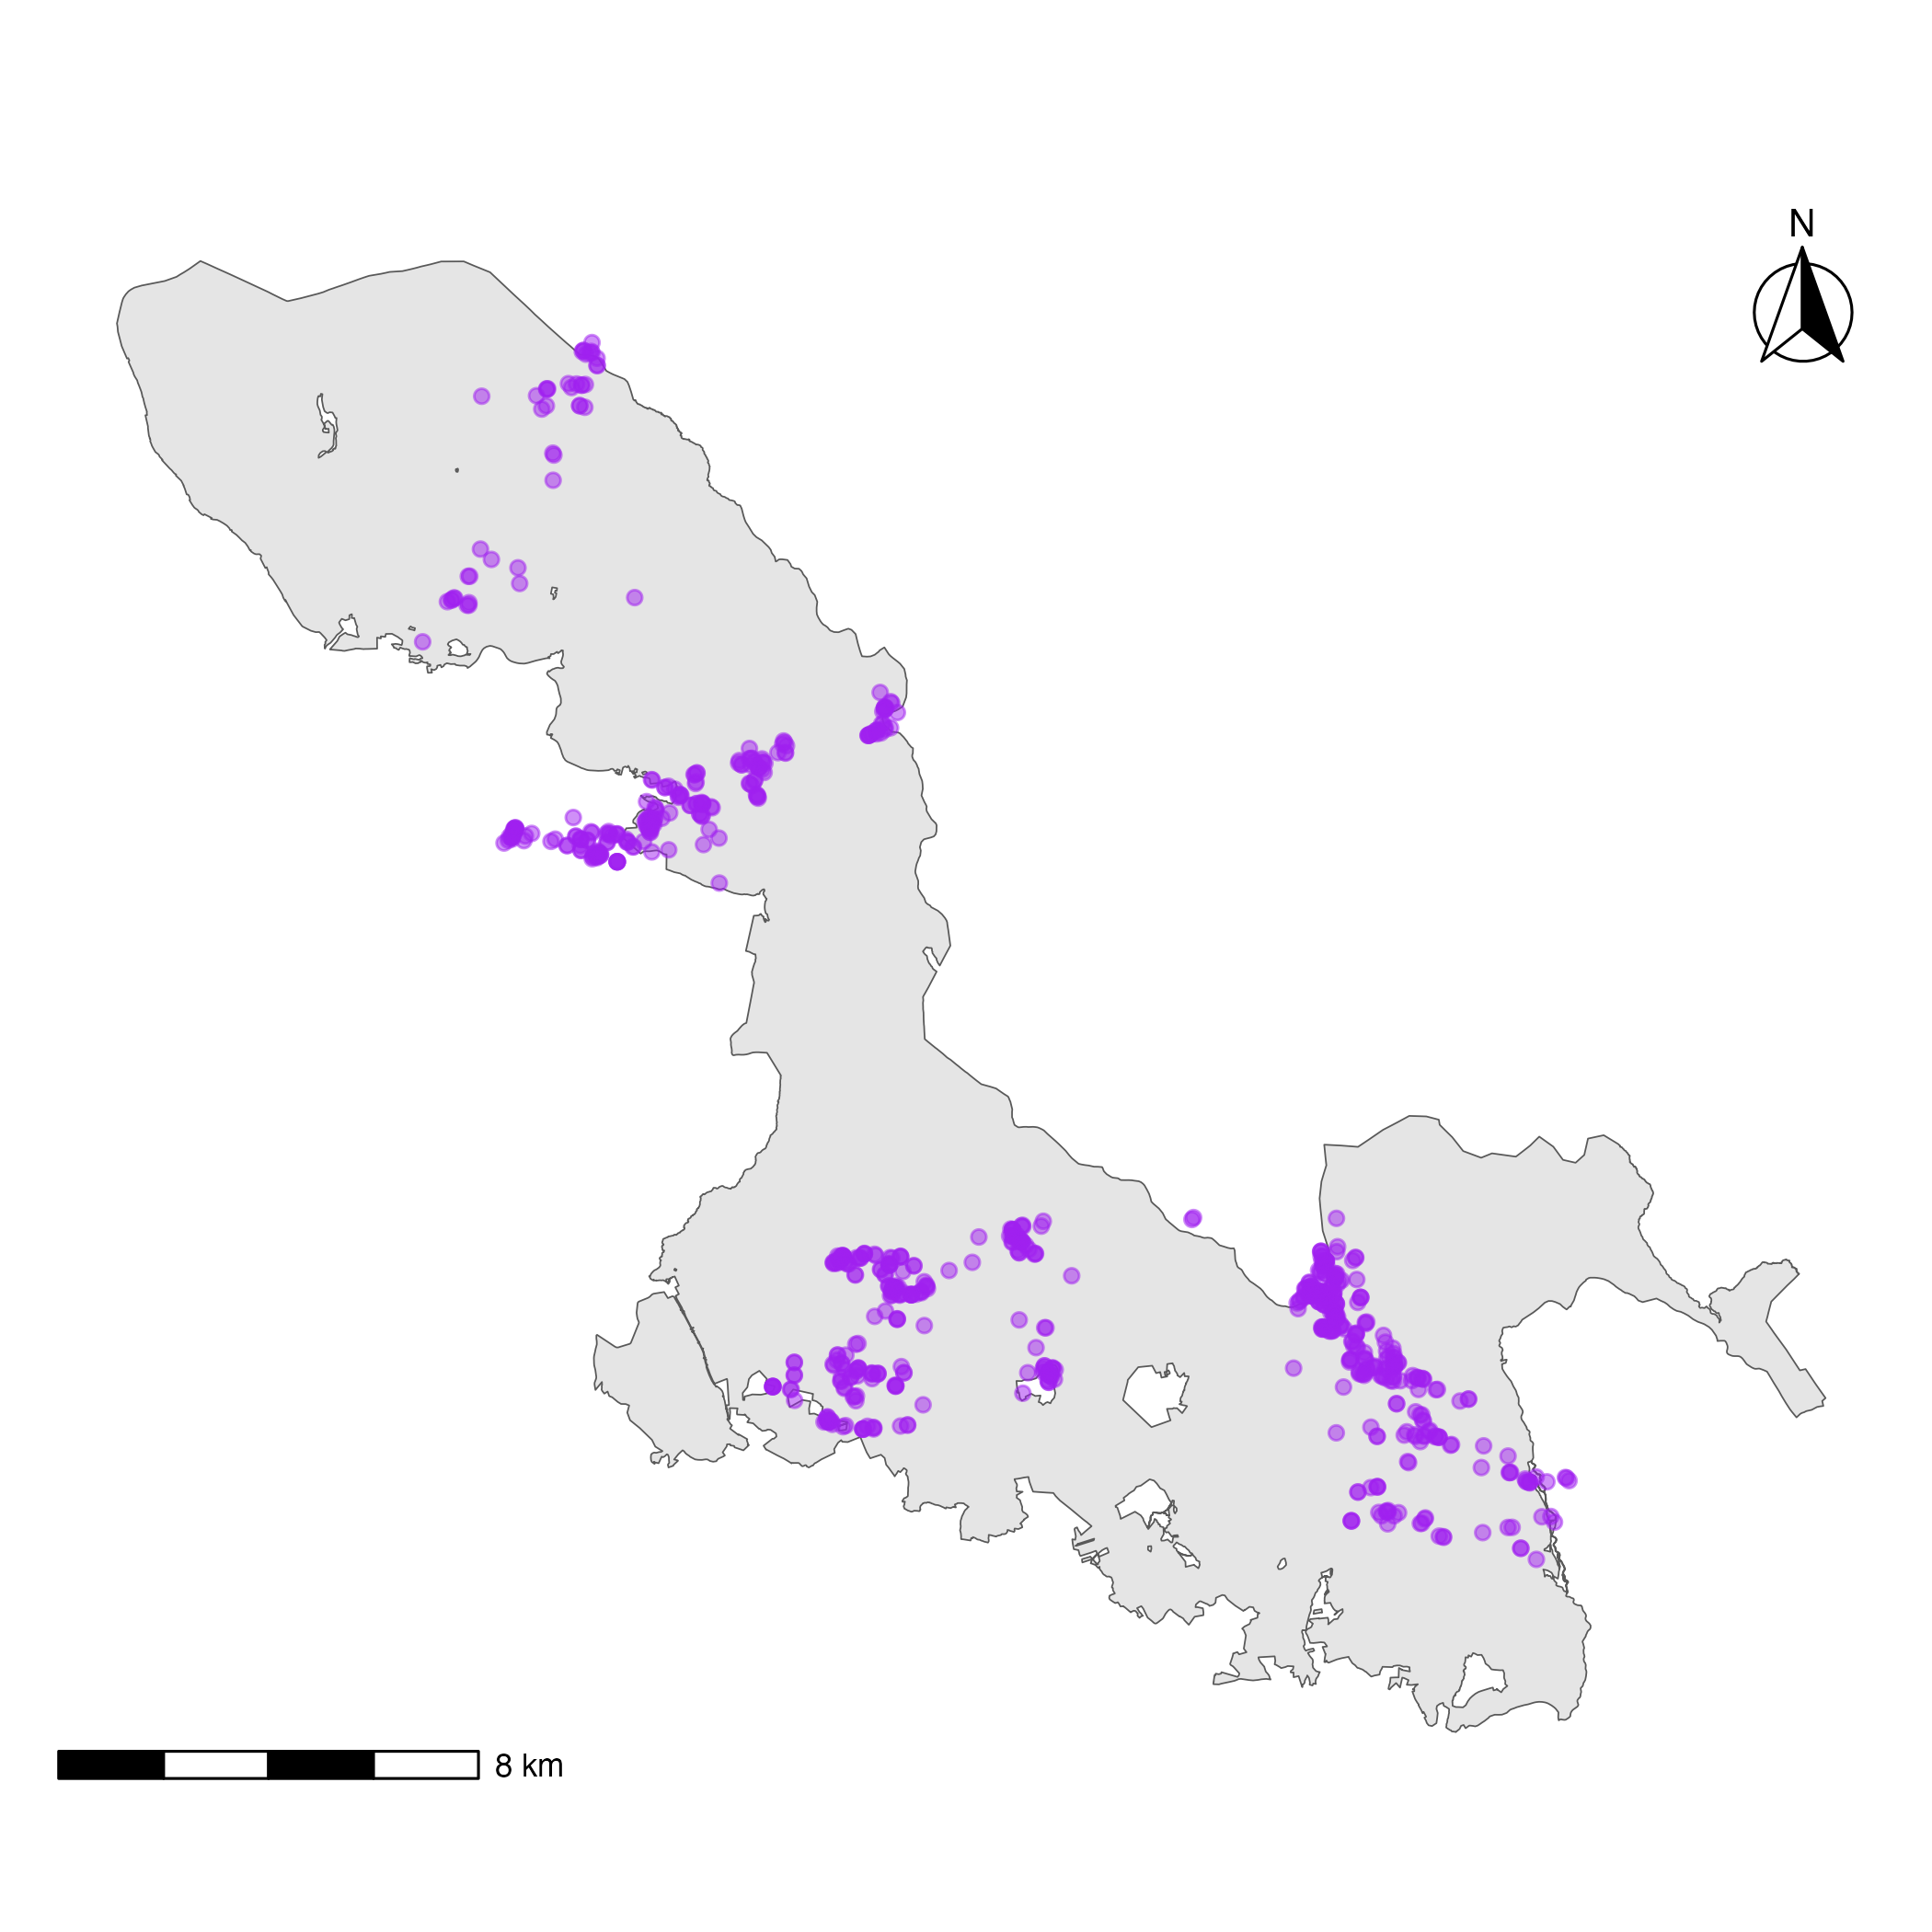
\includegraphics[keepaspectratio]{Figures/sp_samples.png}}

}

\caption{\label{fig-samples_locations}Samples - Locations}

\end{figure}%

\section{Reproduction Data}\label{reproduction-data}

The reproduction data contains reproduction information on some of the
deers. It has not been used in our analysis and modelling approach, for
the reasons see Section~\ref{sec-feature_selection}.

\chapter{Data Preprocessing}\label{data-preprocessing}

The datasets undergo preprocessing steps to facilitate analysis and
modelling:

\begin{itemize}
\tightlist
\item
  Convertion of Timestamps and Coordinates to a uniform format
\item
  Removal of entries with missing values (especially timestamps), zeros,
  or highly implausible data
\end{itemize}

Each FCM sample gets associated with all hunting events occurring before
the sample was produced. The resulting dataset containes samples linked
to all prior hunting events, creating multiple pairings per sample.

\section{Filtering}\label{sec-filtering}

A hunting event and a deer are separated by both space and time.
Therefore we define the essential covariates to be:

\begin{enumerate}
\def\labelenumi{\roman{enumi})}
\tightlist
\item
  \emph{Time Difference} between the hunting event and the subsequent
  defecation
\item
  \emph{Spatial Distance} between a deer and the hunting event at the
  exact time of the event
\end{enumerate}

Additionally we identify other covariates:

\begin{enumerate}
\def\labelenumi{\roman{enumi})}
\setcounter{enumi}{2}
\tightlist
\item
  Time Difference between defecation and sampling (\emph{Sample Delay})
\item
  Day of year {[}1-365{]}\footnote{Not all values between 1 and 365 were
    observed. As shown in Figure~\ref{fig-samples_daily_count}, faecal
    samples were not collected during winter.} (\emph{Defecation Day})
\item
  Number of hunts a deer experiences before defecation (\emph{Number of
  Other Hunts})
\end{enumerate}

While each faecal sample can be associated with one or more hunting
events prior to defecation, we do not use all possible pairings for our
analysis. Suppose two hunting events occured before a deer defecated.
The first hunting event occurred, say, 3 days prior to defecation, and
the second event occurred 20 hours prior to defecation. According to
Huber et al. (2003), the FCM level increases as stress response, but
this increase is short-term (see also Figure~\ref{fig-fcm}). If we did
observe an increase of FCM level, this increase should predominantly be
associated with the second hunting event. However, this assumption is
only reasonable, if both hunting events had a small distance to the
deer, as we expect far way hunting events to have little influence. With
both temporal and spatial distance in mind, we focus on the \emph{most
relevant hunting event} for each faecal sample and propose the following
definitions for this notion:

\begin{enumerate}
\def\labelenumi{\arabic{enumi}.}
\item
  \emph{Closest in time}: Choosing the hunting event, which happened
  closest to 19 hours prior to the defecation event. This takes the
  findings of Huber et al. (2003) into account, that cortisol metabolite
  concentrations peak around 19 hours post-stress event (see
  Figure~\ref{fig-fcm}).
\item
  \emph{Nearest}: Choosing the observation with the shortest spatial
  distance between the hunting event and the deer's interpolated
  position at the time of the hunting event.
\item
  \emph{Highest score}: Introducing a scoring function to consider both
  spatial and temporal distance. We designed a score proportional to the
  inverse square of the distance and a ``spike'' function based on Time
  Difference (see Figure~\ref{fig-score}). The inverse square component
  is inspired by the inverse square law for sound intensity, spike
  function was inspired by the general dynamics of stress responses,
  incorporating insights from Huber et al. (2003), and Piñero et al.
  (2025). The observation with the highest score was selected. The
  scoring function is precisely given by \begin{equation*}
    S(d, t) \propto \frac{1}{d^2} \cdot \begin{cases}
    f_\textbf{t}(t), \hspace{.1cm} \textbf{t} \sim \mathcal{N}(\mu, \sigma^2) &t \leq \mu \\
    f_\textbf{t}(t), \hspace{.1cm} \textbf{t} \sim \mathcal{Laplace}(\mu, b) &t > \mu,
    \end{cases}
  \end{equation*} where \(d\) is the spatial distance, \(t\) the Time
  Difference between hunting and defecation event, while \(\mu = 19\),
  once again incoporates Huber et al. (2003) findings. \(\sigma = 2\)
  and \(b = 2.5\) are shape paramters.
\end{enumerate}

\begin{figure}

\centering{

\pandocbounded{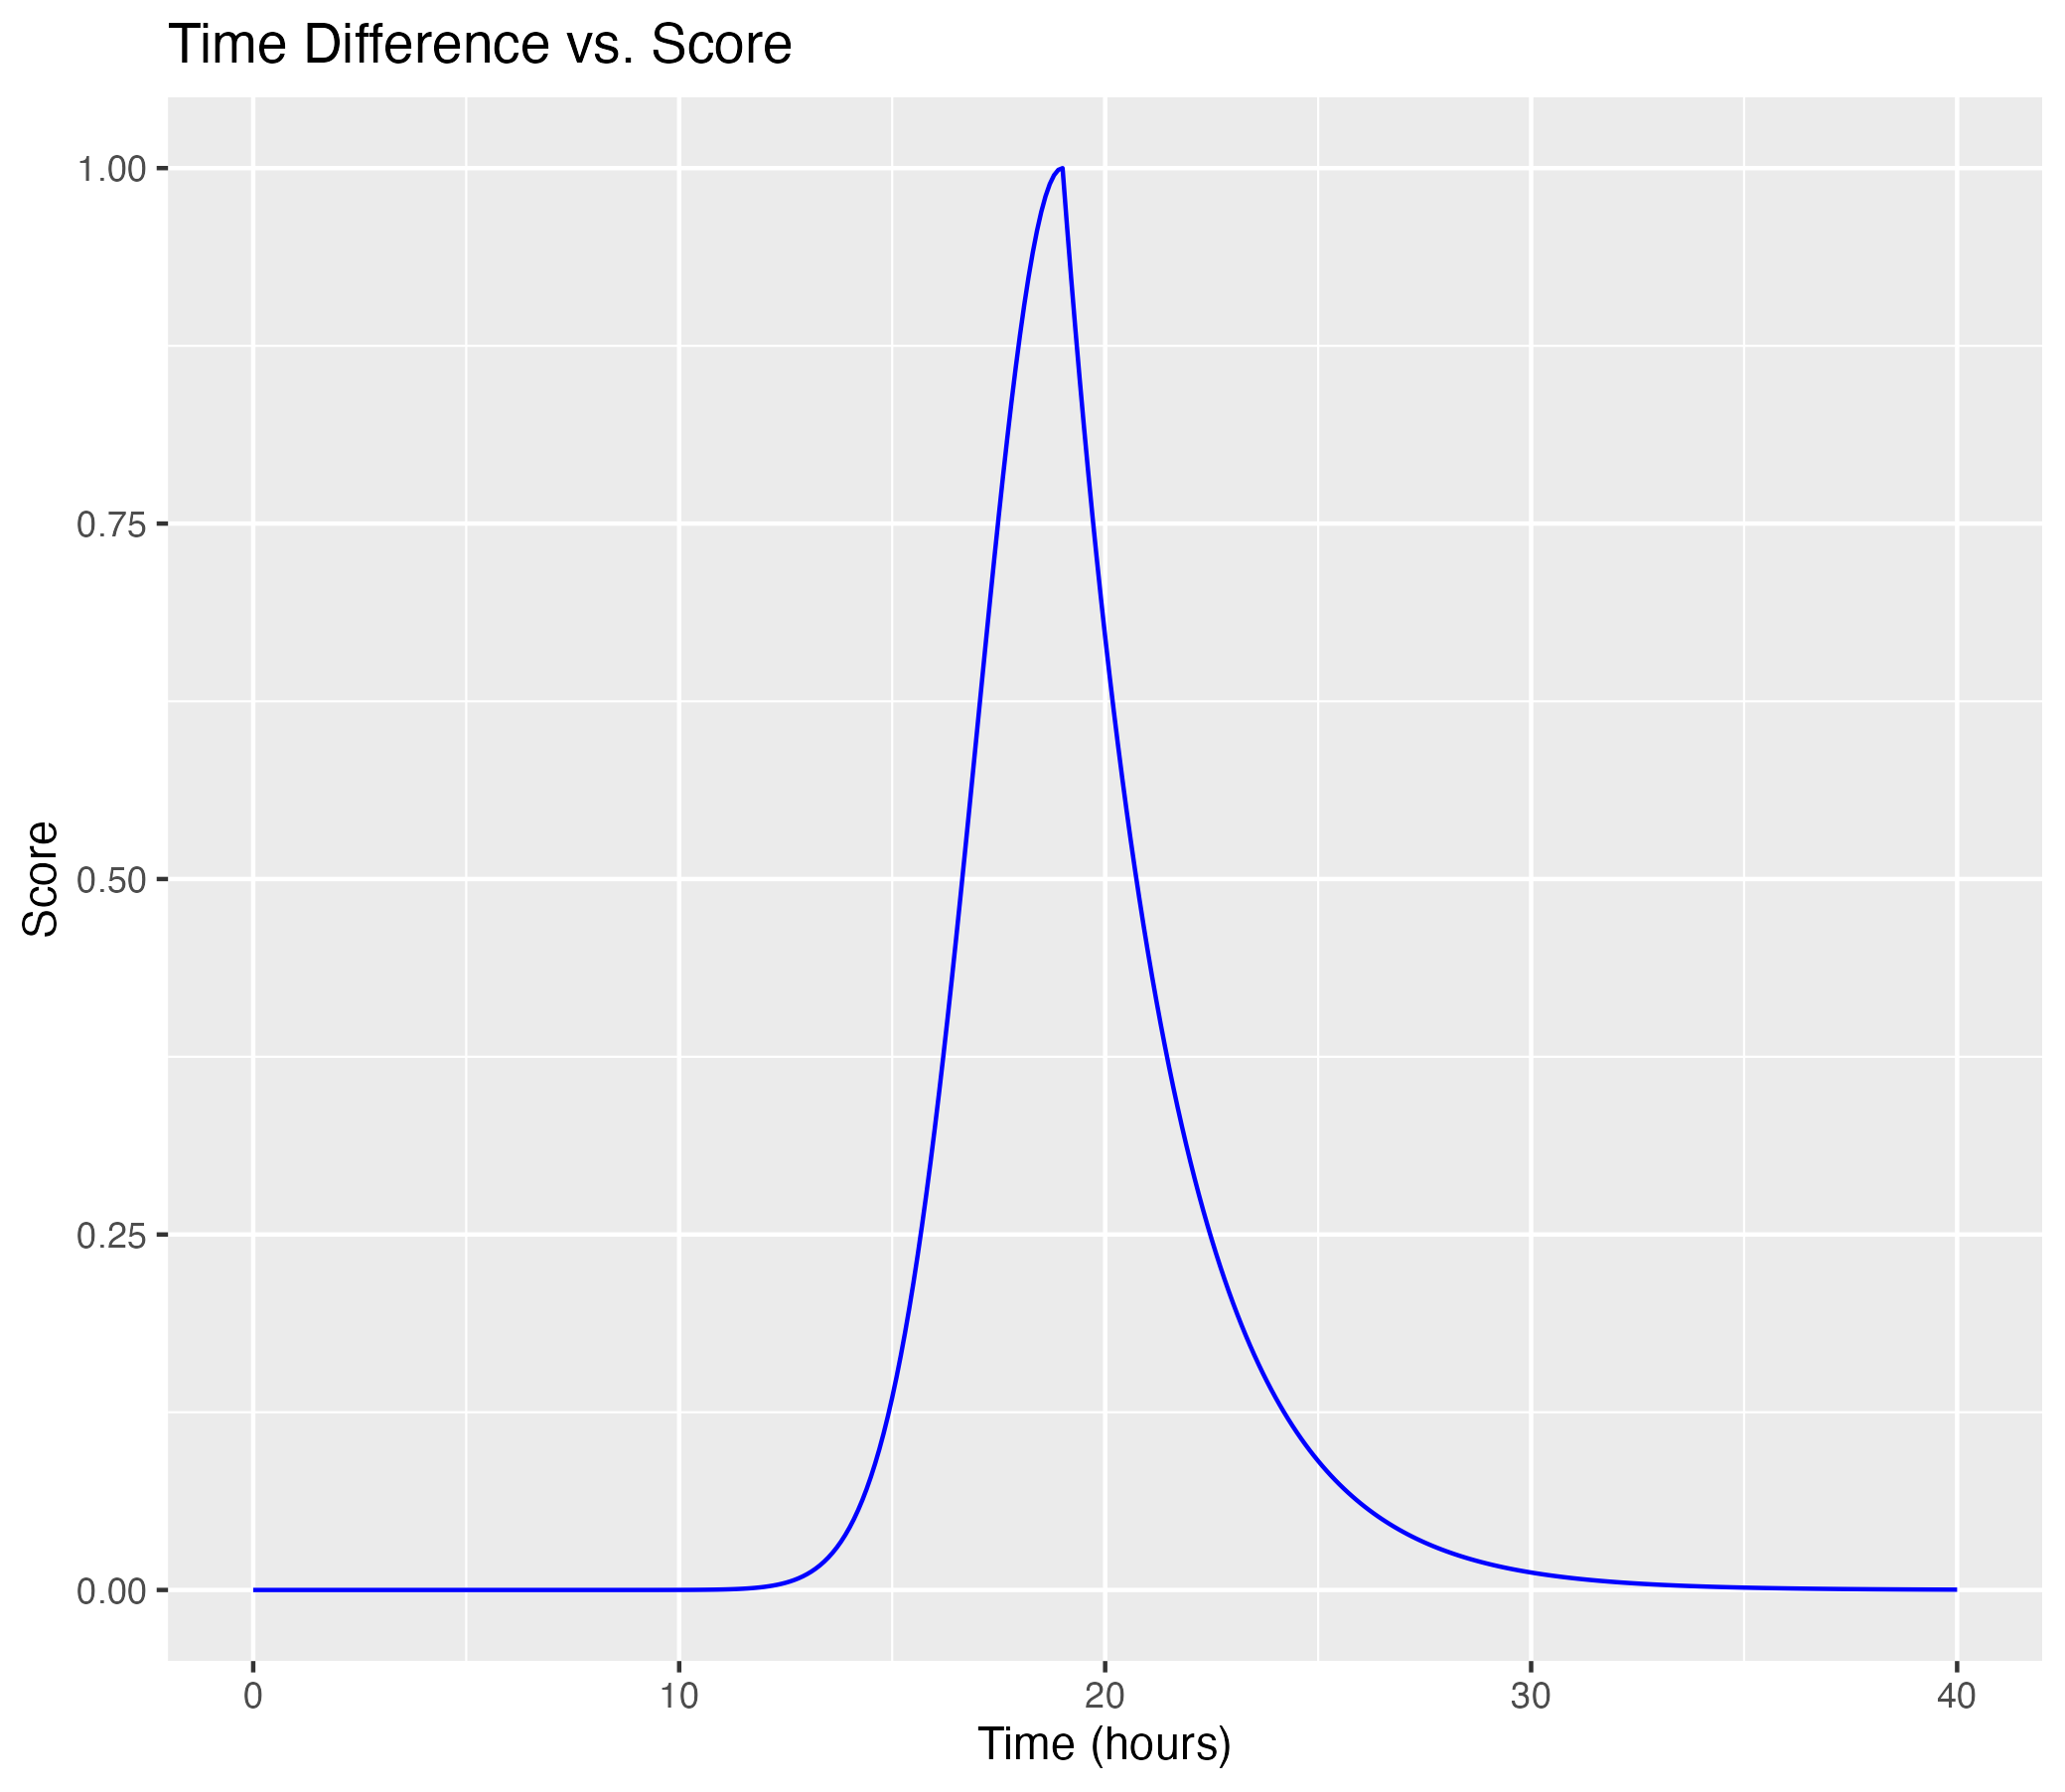
\includegraphics[keepaspectratio]{Figures/Timediff_Function_impact_curve.png}}

}

\caption{\label{fig-score}Score Function}

\end{figure}%

Having identified the most relevant hunting event, covariate i) can be
calculated easily as the time difference between the hunting event and
the defecation event. To obtain covariate ii) we have to take in
account, that the movement data is recorded in 1-hour intervals, while
the hunting events occur at arbitrary time points. Therefore we need to
approximate the exact deer positions at hunting event times. We
interpolate deer positions at the timestamp of each hunting event,
assuming constant velocity and linear movement. Suppose a hunting event
occurred at time \(t\), but we only know the deer's location at time
\(t_0, t_1\) with \(t_0 < t < t_1\). Then we approximate the location
\(r(t)\) of the deer at time \(t\) by \begin{equation*}
  r(t) \approx r(t_0) + \frac{t - t_0}{t_1 - t_0} (r(t_1) - r(t_0)),
\end{equation*} where \(r(t_0)\) and \(r(t_1)\) denote the recorded
locations of the deer at time \(t_0\) and \(t_1\), respectively. We
define covariate ii) to be the distance between the approximated deer
location and the location of the hunting event. In cases where the time
point of a movement recording coincides with that of a hunting event, we
use the exact distance.

Covariates iii) and iv) are again easy to obtain. For covariate v), we
need to define a cutoff point in time and space, to identify which other
hunting events could have affected a deer as well (see
Table~\ref{tbl-thresholds}).

\begin{table}

\caption{\label{tbl-thresholds}The three proposed DataSets. For each
DataSet, \emph{Temporal} refers to the upper limit of Time Difference
between Hunting Event an Defecation Event, with the lower limit beeing
zero. \emph{Spatial} refers to the upper limit of the distance between
deer and Hunting event, with the lower beeing zero as well.}

\centering{

\centering\begingroup\fontsize{10}{12}\selectfont

\begin{tabular}{l|r|r}
\hline
DataSet & Temporal [h] & Spatial [km]\\
\hline
Closest in time & 36 & 10\\
\hline
Nearest & 36 & 10\\
\hline
Highest score & 200 & 15\\
\hline
\end{tabular}
\endgroup{}

}

\end{table}%

\section{Uncertainties}\label{uncertainties}

A major challenge in our analysis is the large uncertainty in data which
propogates through the pre-processing steps into our models.

First, the uncertainty about spatial distances between deer and hunting
events is large. While the movement of deer was tracked at hourly
intervals, hunting events occurred irregularly. In our
interpolation-based approximation of a deer's location at the time of
hunting event, the approximation error is unknown.

Second, we have very limited information for addressing the short-term
stress response of the deer. On the one hand, the available data contain
only 500 hunting events with complete time and location information
scattered across a 30km \(\times\) 30km area in the span of two years.
The observed hunting events only populate the space-time scarcely. On
the other hand, we observe in Figure~\ref{fig-deers_locations} that the
deer tended to roam around within a small area. As a result, each deer
is likely to have only encountered very few hunting events at small
spatial and temporal distances.

Third, there could be a large number of confounders for which we possess
no information. Based on GPS coordinates, we can compute Euclidean
distances between deer and hunting events. However, we cannot account
for terrain and vegetation which could affect the propagation of sound
and therefore contaminate the potential effect of hunting events.
Furthermore, there could be unobserved stress stimuli, such as weather
conditions, predators, and human activities other than hunting.

Fourth, we assumed that each hunting event was actually a sound event
(i.e.~a shot was fired). Therefore, we weighted the value of our score
function by the inverse square distance.

\chapter{Model Selection}\label{model-selection}

To address how the FCM level depends on Time Difference and spatial
distance, we follow a statistical approach for interpretability and a
machine learning approach for exploration. In this section, we present
details on model specification. Both approaches use all the datasets
shown in Table~\ref{tbl-datasets}.

\begin{table}

\caption{\label{tbl-datasets}Count of individual deer and faecal sample
for each of the proposed DataSets.}

\centering{

\centering\begingroup\fontsize{10}{12}\selectfont

\begin{tabular}{r|r|r}
\hline
DataSet & Deer & Observations\\
\hline
Closest in time & 35 & 149\\
\hline
Nearest & 35 & 147\\
\hline
Highest score & 36 & 223\\
\hline
\end{tabular}
\endgroup{}

}

\end{table}%

\section{Statistical modeling approach}\label{sec-stat_model}

For each dataset shown in Table~\ref{tbl-datasets}, we consider the five
covariates introduced in Section~\ref{sec-filtering}.

The \emph{Time Difference} and \emph{spatial distance} are of main
interest for our first research question. The effect of \emph{sample
delay} is the subject of our second research question. We consider the
\emph{day of defecation} as a potential confounder, as the deer's stress
level exhibits seasonal patterns (Vilela et al. 2020). The \emph{number
of other relevant hunting events} reflects the intensity of recent
hunting activity. In time periods of frequent hunting events, a deer
might have a generally higher stress level, or adaptation might occur
which dampens the stress response towards new hunting events.

We propose a generalized additive mixed model (GAMM) to account for
potentially non-linear effects of covariates and potential individual
differences between the observed deer. We use the R package
\texttt{mgcv} (Wood 2011) to fit the models. The covariates Time
Difference, Distance, Sample Delay, and Defecation Day are encoded by
penalized cubic regression splines. We do not use a cyclical spline for
Defecation Day, because faecal samples were not collected during winter
and therefore Defecation Day is not a cyclical variable. The Number of
Other Relevant Hunting Events is adopted as a linear effect. We further
introduce a random intercept for each deer.

For the distributional assumption, we use the Gamma family with a log
link. Since the FCM level is non-negative, we expect the Gamma
assumption to more appropriate than Gaussian. A full specification of
our GAMM model is as follows. Let \(i = 1,\dots,N\) be the indices of
the deer and \(j = 1,\dots,n_i\) be the indices of faecal samples for
each deer \begin{align*}
  \textup{FCM}_{ij} &\overset{\mathrm{iid}}{\sim} \mathcal{Ga}\left( \nu, \frac{\nu}{\mu_{ij}} \right) \quad\text{for}\; j = 1,\dots,n_i, \\
  \mu_{ij} &= \mathbb{E}(\textup{FCM}_{ij}) = \exp(\eta_{ij}), \\
  \eta_{ij} &= \beta_0 \\
  &+ \beta_1 \textup{Number of Other Hunts}_{ij} \\
  &+ f_1(\textup{Time Difference}_{ij}) + f_2(\textup{Distance}_{ij}) \\
  &+ f_3(\textup{Sample Delay}_{ij}) + f_4(\textup{Defecation Day}_{ij}) \\
  &+ \gamma_{i}, \\
  \gamma_i &\overset{\mathrm{iid}}{\sim} \mathcal{N}(0, \sigma_\gamma^2),
\end{align*} where \(f_1, f_2, f_3, f_4\) are penalized cubic regression
splines, \(\sigma_\gamma^2 > 0\), and \(\nu > 0\).

Our model has two major limitations. First, it does not account for
potential interactions between the covariates. Second, the random
intercept term can only capture different base stress levels, but not
differences in stress response. However, given the limited data, one
must trade off between model complexity and stability in estimation. In
fact, our current model already exhibits instability with respect to
estimation procedures, which we discuss in Chapter~\ref{sec-results}.

\section{Machine learning approach}\label{machine-learning-approach}

Chen and Guestrin (2016) introduced XGBoost as a machine learning
algorithm that improves prediction accuracy by building an ensemble of
decision trees sequentially. Each new tree corrects the errors made by
previous trees. XGBoost minimizes a loss function using gradient
boosting (hence the name) by iteratively adding trees that best reduce
the residual errors. Simultaneously, complexity gets penalized through
regularization to prevent overfitting. A major feature of XGBoost is
that it doesn't require specifying a parametric relationship between
target and explanatory variables.

We propose a xgboost model using the R package \texttt{xgboost} (Chen et
al. 2024), choosing \emph{spatial distance} and \emph{Time Difference}
as covariates. To find the best fitting model for each dataset (see
Table~\ref{tbl-datasets}), we tune hyperparamters of the proposed
xgboost model. We choose to tune the following paramters, using
randomized grid search (Bergstra and Bengio 2012):

\begin{itemize}
\tightlist
\item
  \emph{maximum depth}:~ Controls the maximum depth of each decision
  tree, determining how complex each tree can become.
\item
  \(\eta\):~ The learning rate, controls how much each new tree
  contributes to the ensemble, affecting how quickly or cautiously the
  model learns.
\item
  \(\gamma\):~ The minimum loss reduction required to make a split,
  acting as a regularization parameter that prevents creating splits
  that don't significantly improve the model.
\item
  \emph{subsample}:~ Specifies the fraction of training data used to
  build each tree, introducing randomness to prevent overfitting.
\item
  \emph{features by tree}:~ Determines the fraction of features
  (columns) randomly sampled for each tree, increasing diversity among
  trees.
\item
  \emph{minimum weight of child}:~ Minimum sum of instance weight needed
  in a child node, helping control the complexity of the model by
  preventing overly specific partitions.
\end{itemize}

\chapter{Model Evaluation}\label{sec-results}

\section{GAMMs}\label{gamms}

We fitted and evaluated GAMM models across the three datasets, using
REML and GCV as parameter estimation methods. We observed high
instability with respect to the choice of dataset and estimation method.

\begin{figure}

\begin{minipage}{\linewidth}

\pandocbounded{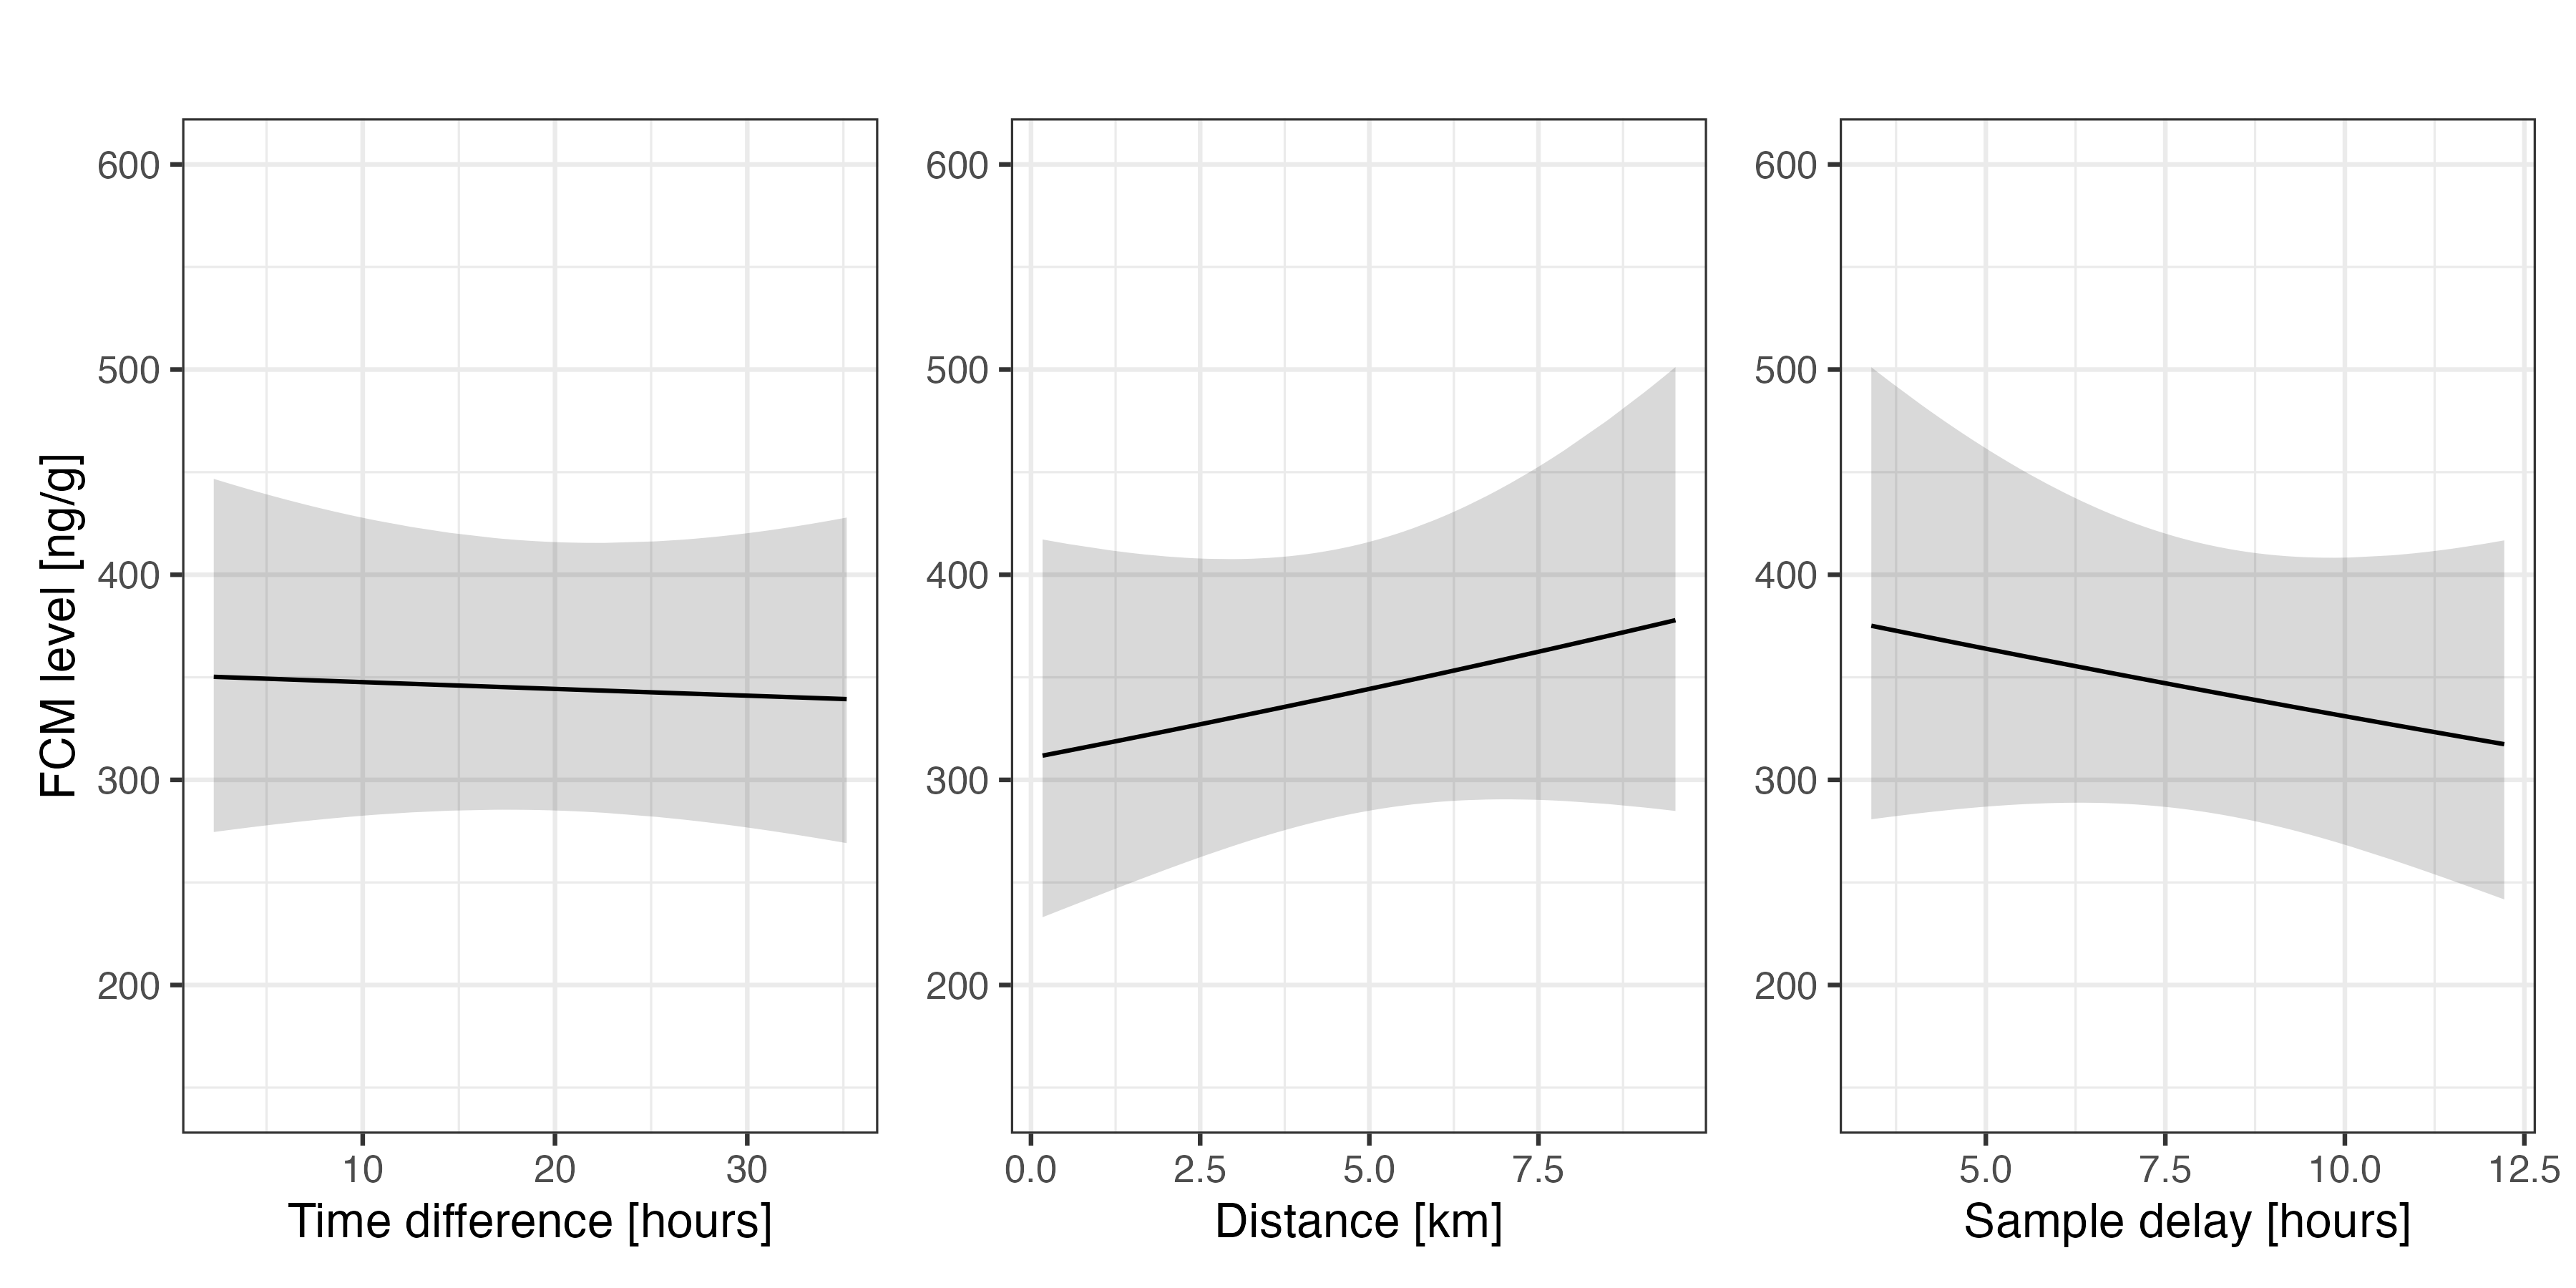
\includegraphics[keepaspectratio]{Figures/Models/last_REML_diagnostic_custom.png}}

\subcaption{\label{}Closest in time.}
\end{minipage}%
\newline
\begin{minipage}{\linewidth}

\pandocbounded{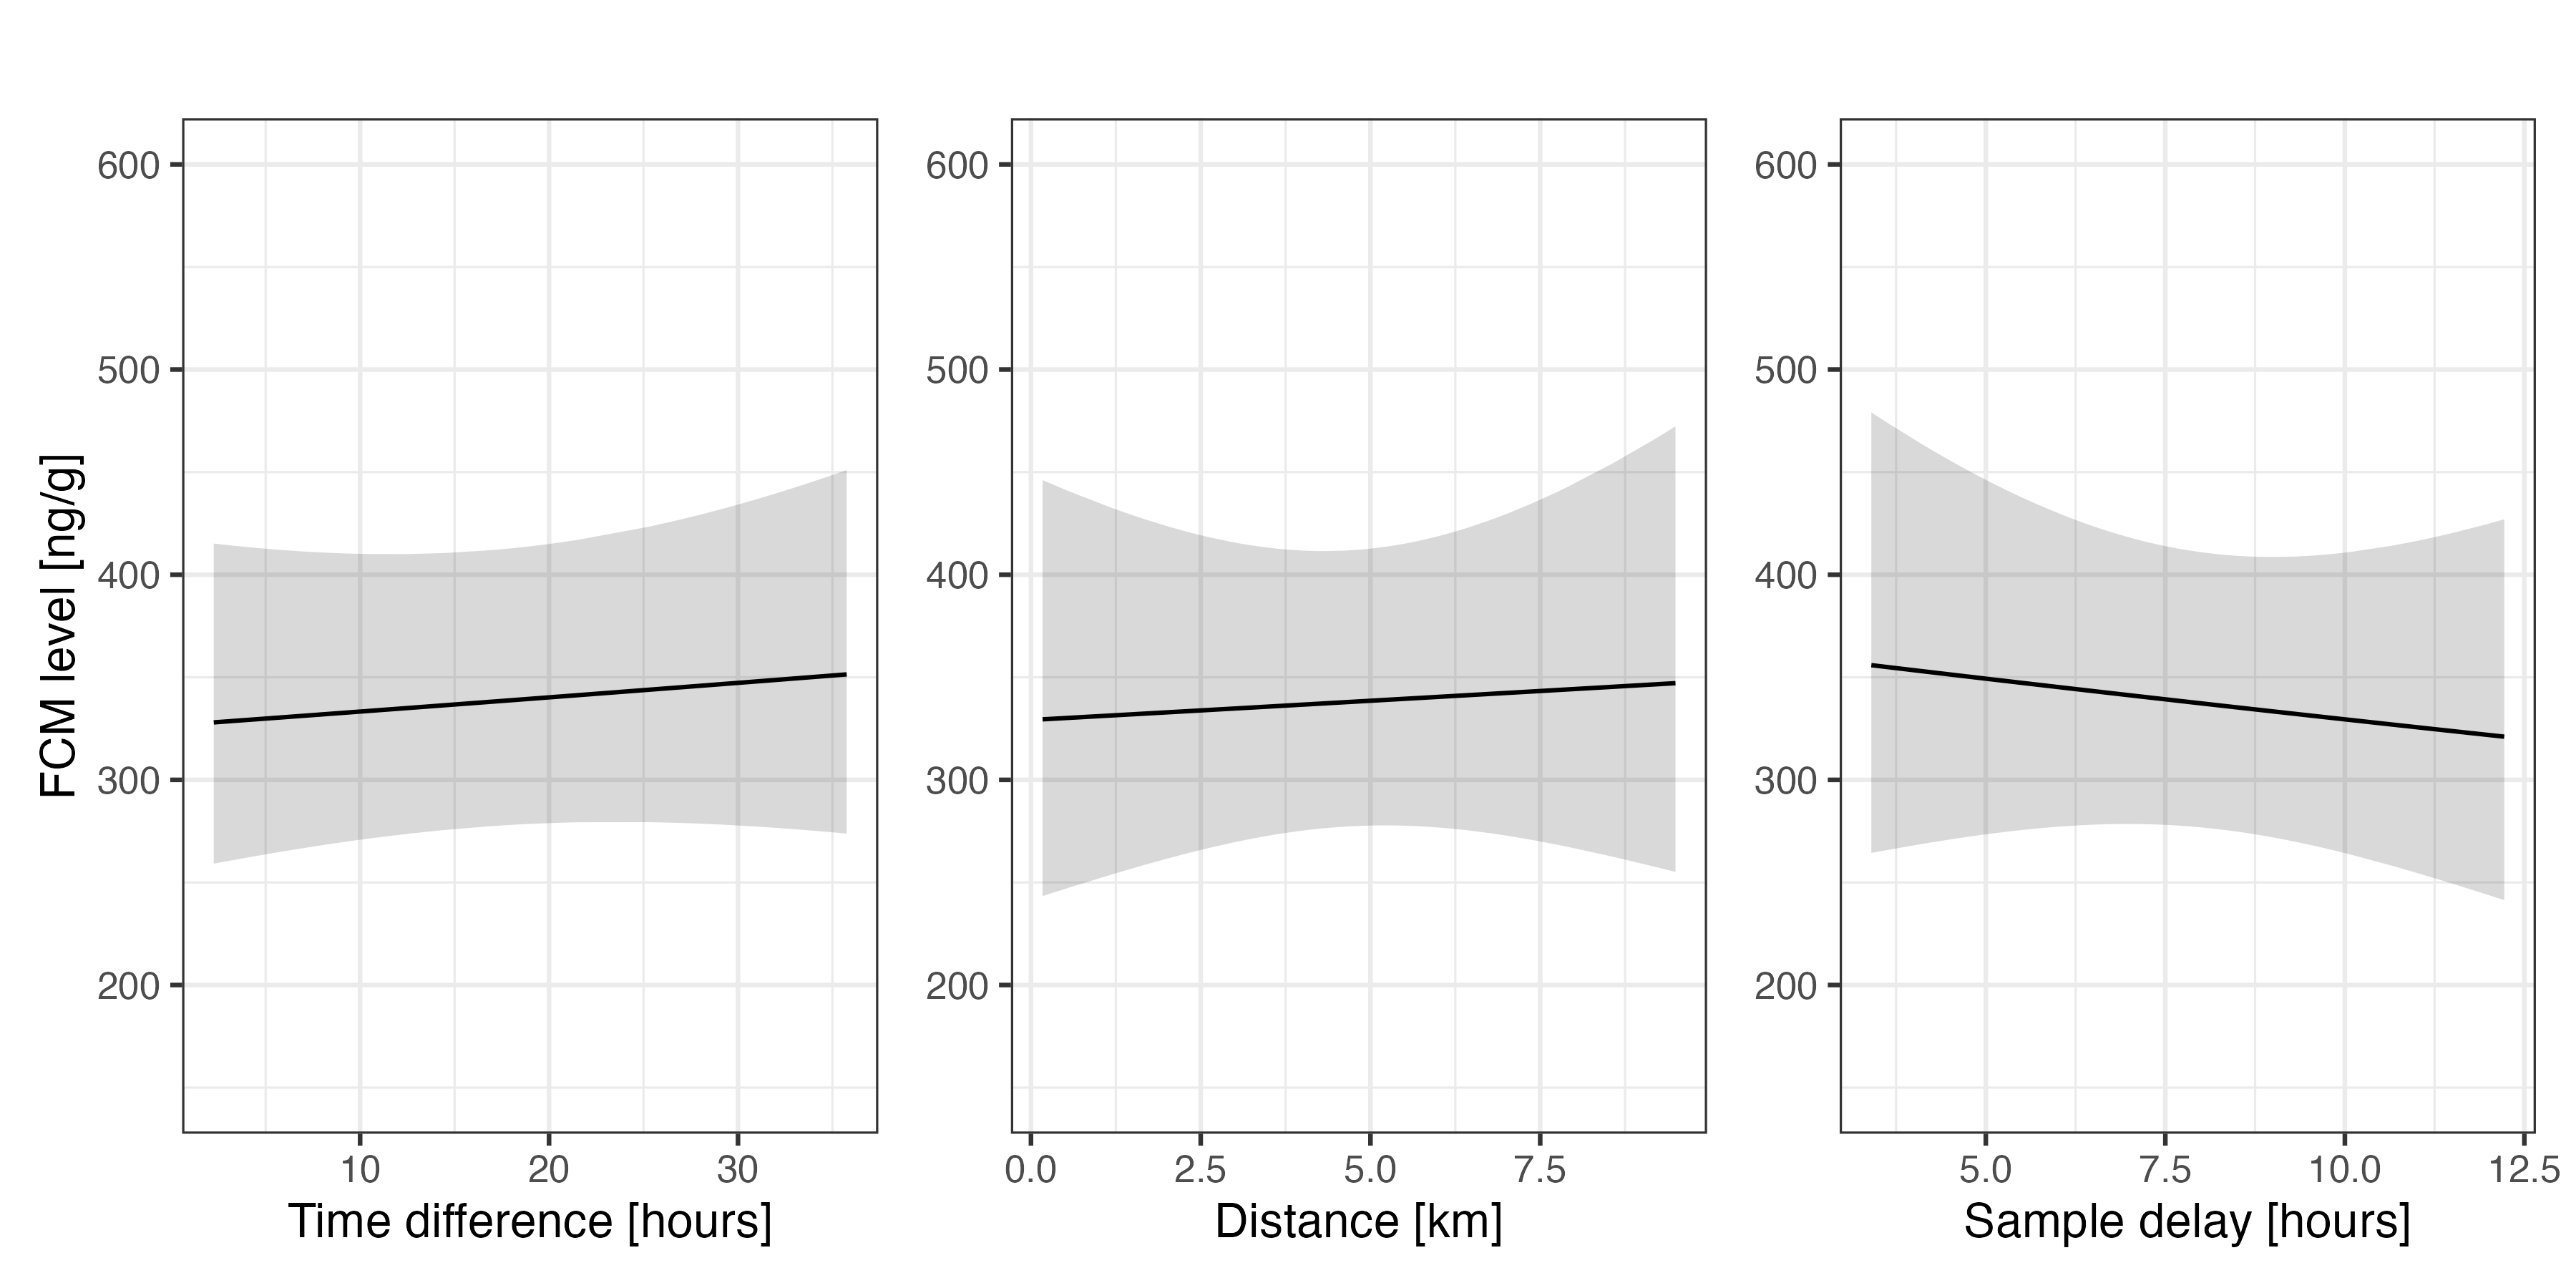
\includegraphics[keepaspectratio]{Figures/Models/nearest_REML_diagnostic_custom.png}}

\subcaption{\label{}Nearest.}
\end{minipage}%
\newline
\begin{minipage}{\linewidth}

\pandocbounded{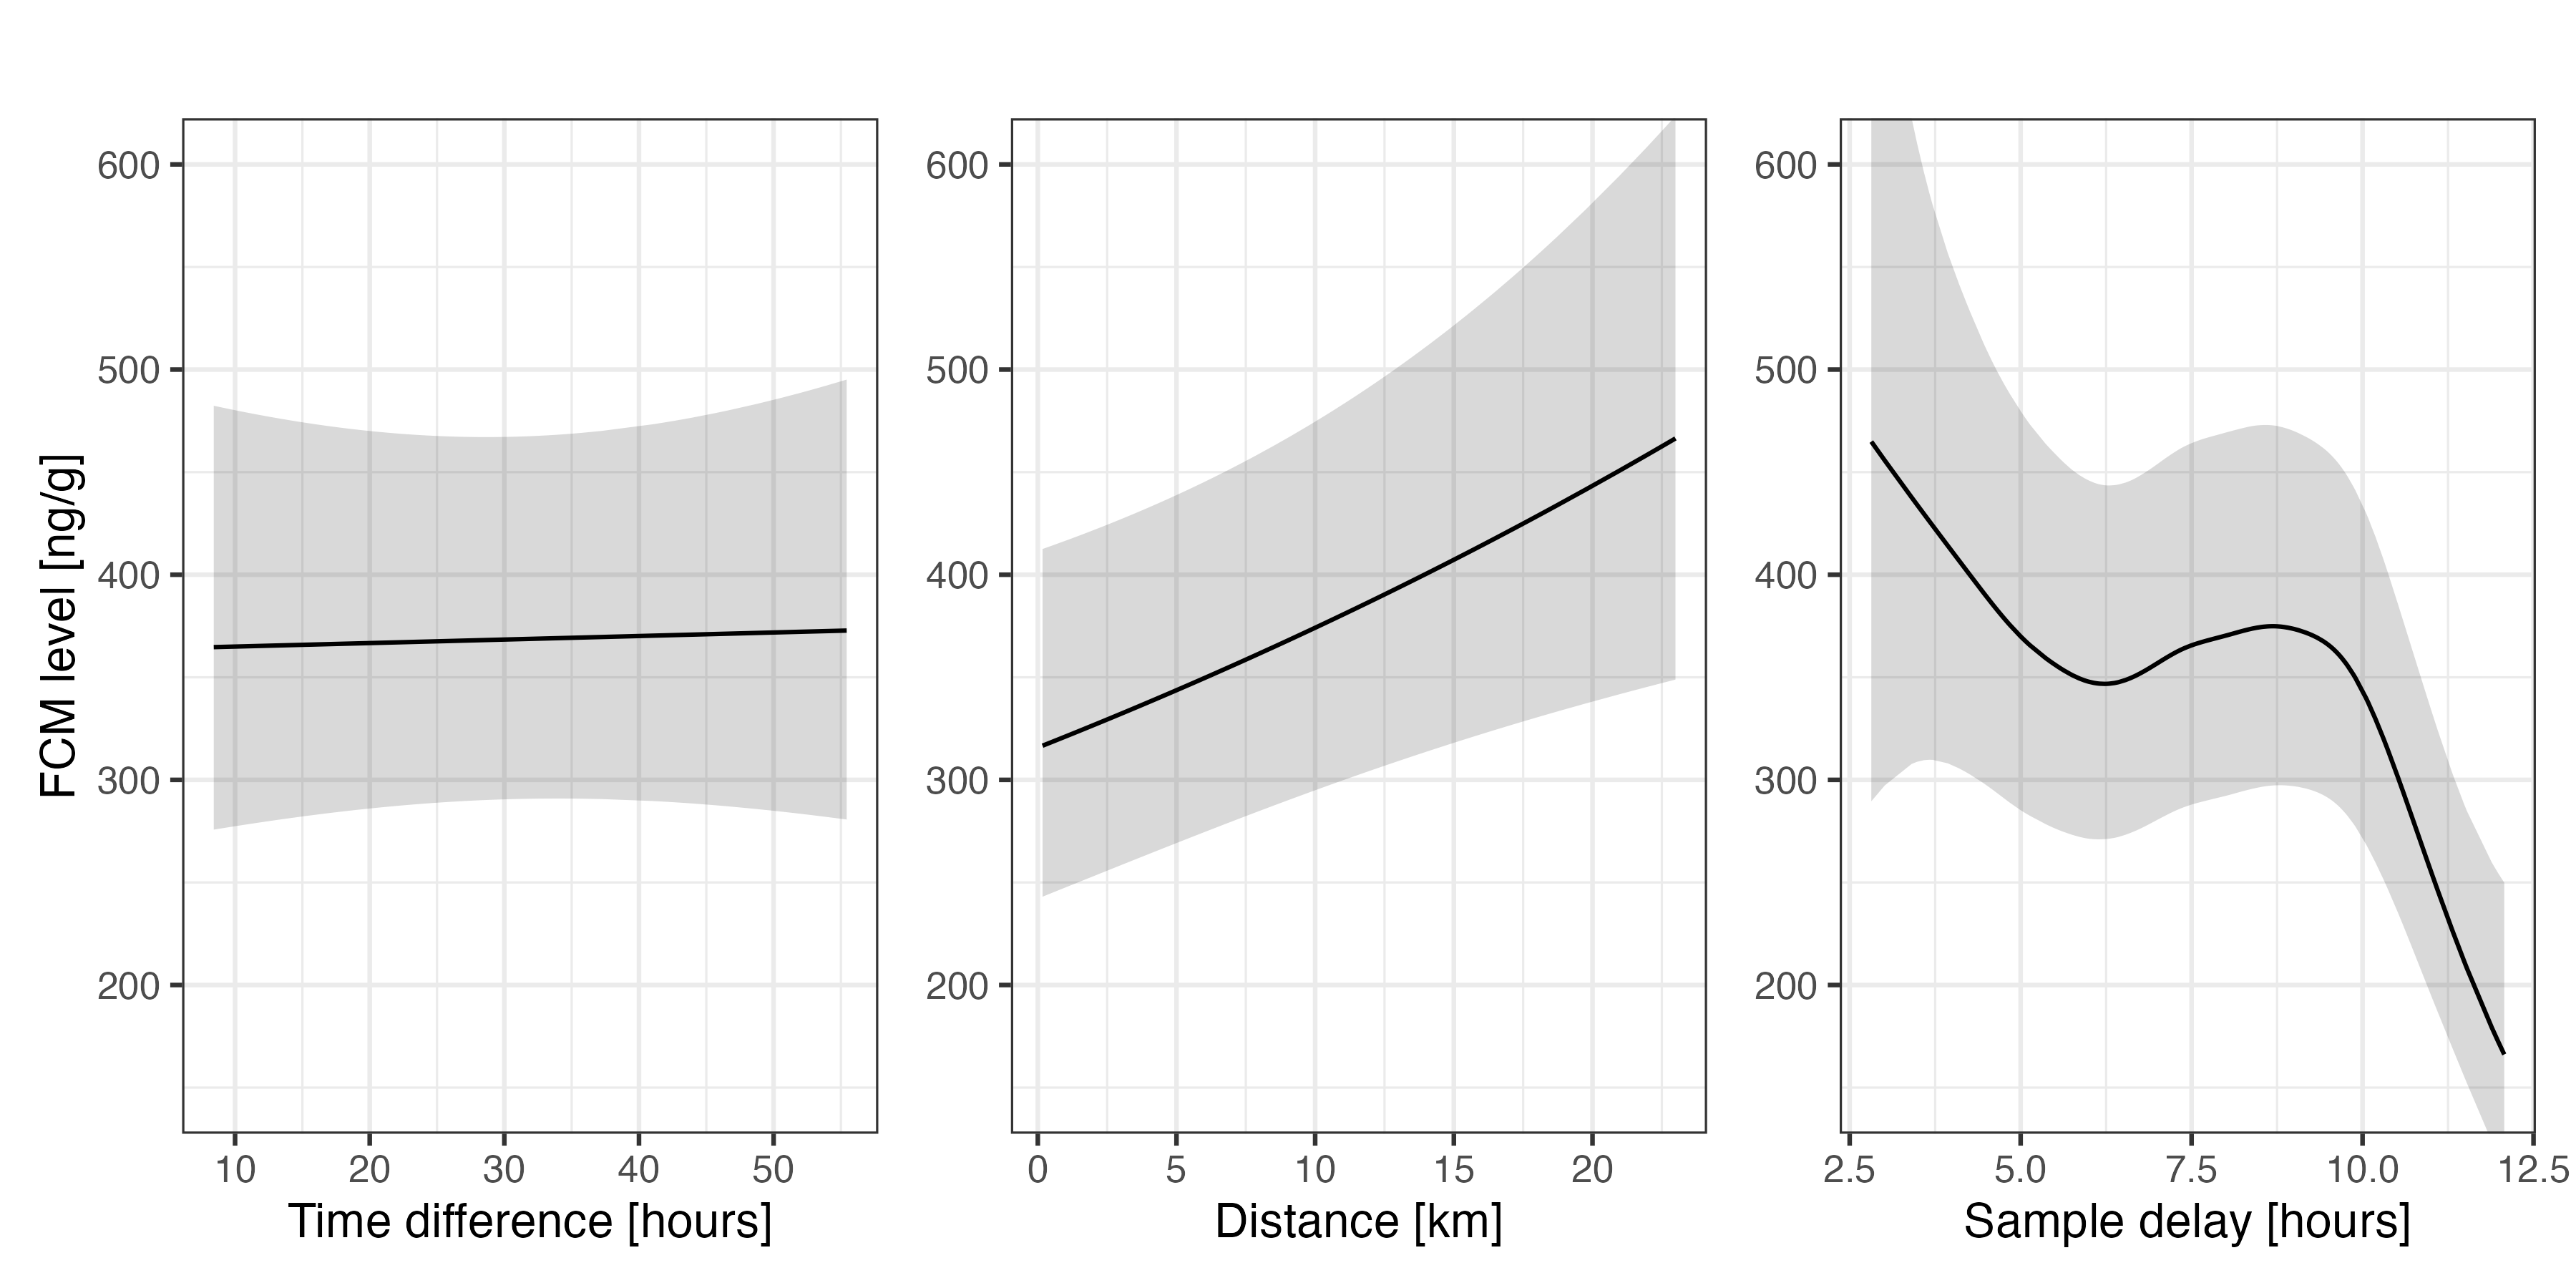
\includegraphics[keepaspectratio]{Figures/Models/score_REML_diagnostic_custom.png}}

\subcaption{\label{}Highest score.}
\end{minipage}%

\caption{\label{fig-gamm-reml}Adjusted predictions for the FCM level on
the three datasets. The GAMM is fitted with the REML method. Each plot
shows the predicted values of the FCM level in dependence of one
covariate. The other covariants are held constant at the mean. The grey
area shows the approximate confidence band (mean \(\pm\) 1.96 standard
error).}

\end{figure}%

In models estimated with the REML method, the smooth effects are
penalized to almost linear, as shown in Figure~\ref{fig-gamm-reml}.
While the fitted curves have a similar tendency across the datasets, the
standard error in estimation is generally high. Given such high
uncertainty, no interpretation of the estimates is reliable. The GCV
method yields more wiggly smooth effect estimates, which are visualized
in Figure~\ref{fig-gamm-gcv}, but high uncertainty persists. For the
other covariates, we also observe high uncertainty and therefore avoid
making any unreliable statement.

On the ``highest score'' dataset which contains more observations than
the other two datasets, both estimation methods agree on a negative
non-linear effect of Sample Delay. This is in accordance with our prior
knowledge that the FCM level in the faecal sample decays after
defecation (Huber et al. 2003).

Similar to the smooth and linear effects, estimation of the
deer-specific random intercepts exhibits high instability. In
particular, the estimated random intercepts differ in order of magnitude
across different dataset (see Figure~\ref{fig-ri}).

\section{XGBoost}\label{xgboost}

The XGBoost model outperforms GAMM on the ``highest score'' and
``nearest'' dataset in terms of model fit measured by root mean squared
error (RMSE), but performs worse on the ``closest in time'' dataset (see
Table~\ref{tbl-rmse}). After reviewing the hyperparameters (see
Table~\ref{tbl-xgboost_hp}) and comparisons between models trained on
the actual data and the data with randomized labels we concluded that
the XGBoost models likely did not learn noise and therefore are not
overfitting.

\begin{table}

\caption{\label{tbl-rmse}Comparison of RMSE between GAMMs and XGBoost
models. The RMSE score is computed on all observations in each dataset.}

\centering{

\centering\begingroup\fontsize{10}{12}\selectfont

\begin{tabular}{r|r|r}
\hline
DataSet & Model & RMSE\\
\hline
Closest in time & GAMM-GCV.Cp & 166.77\\
\hline
Closest in time & GAMM-REML & 178.64\\
\hline
Closest in time & XGBoost & 167.53\\
\hline
Highest score & GAMM-GCV.Cp & 163.69\\
\hline
Highest score & GAMM-REML & 169.76\\
\hline
Highest score & XGBoost & 150.80\\
\hline
Nearest & GAMM-GCV.Cp & 169.50\\
\hline
Nearest & GAMM-REML & 180.20\\
\hline
Nearest & XGBoost & 152.24\\
\hline
\end{tabular}
\endgroup{}

}

\end{table}%

\begin{figure}

\begin{minipage}{\linewidth}

\pandocbounded{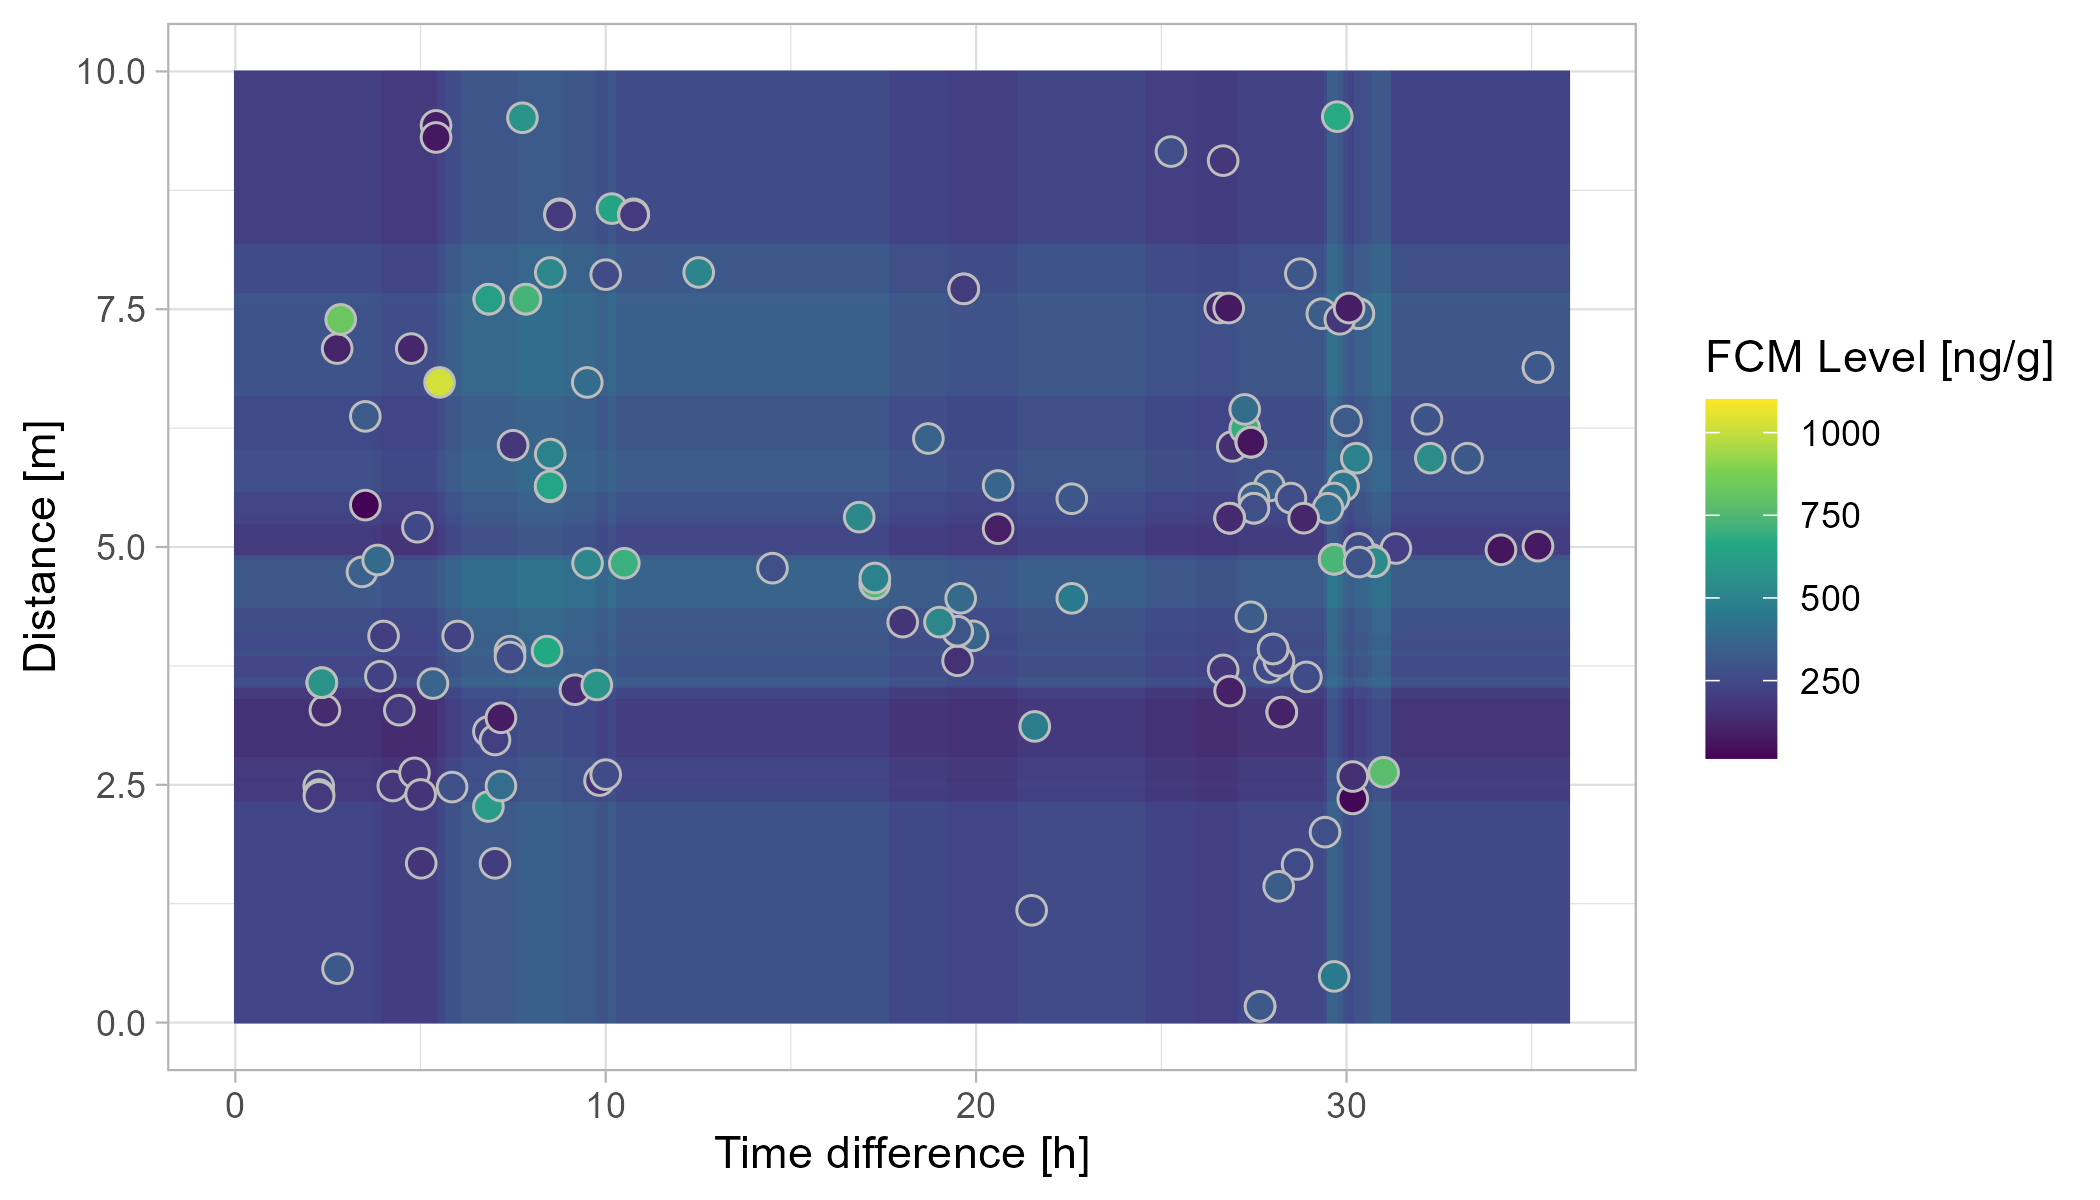
\includegraphics[keepaspectratio]{Figures/Models/xgboost_last.png}}

\subcaption{\label{}Closest in time}
\end{minipage}%
\newline
\begin{minipage}{\linewidth}

\pandocbounded{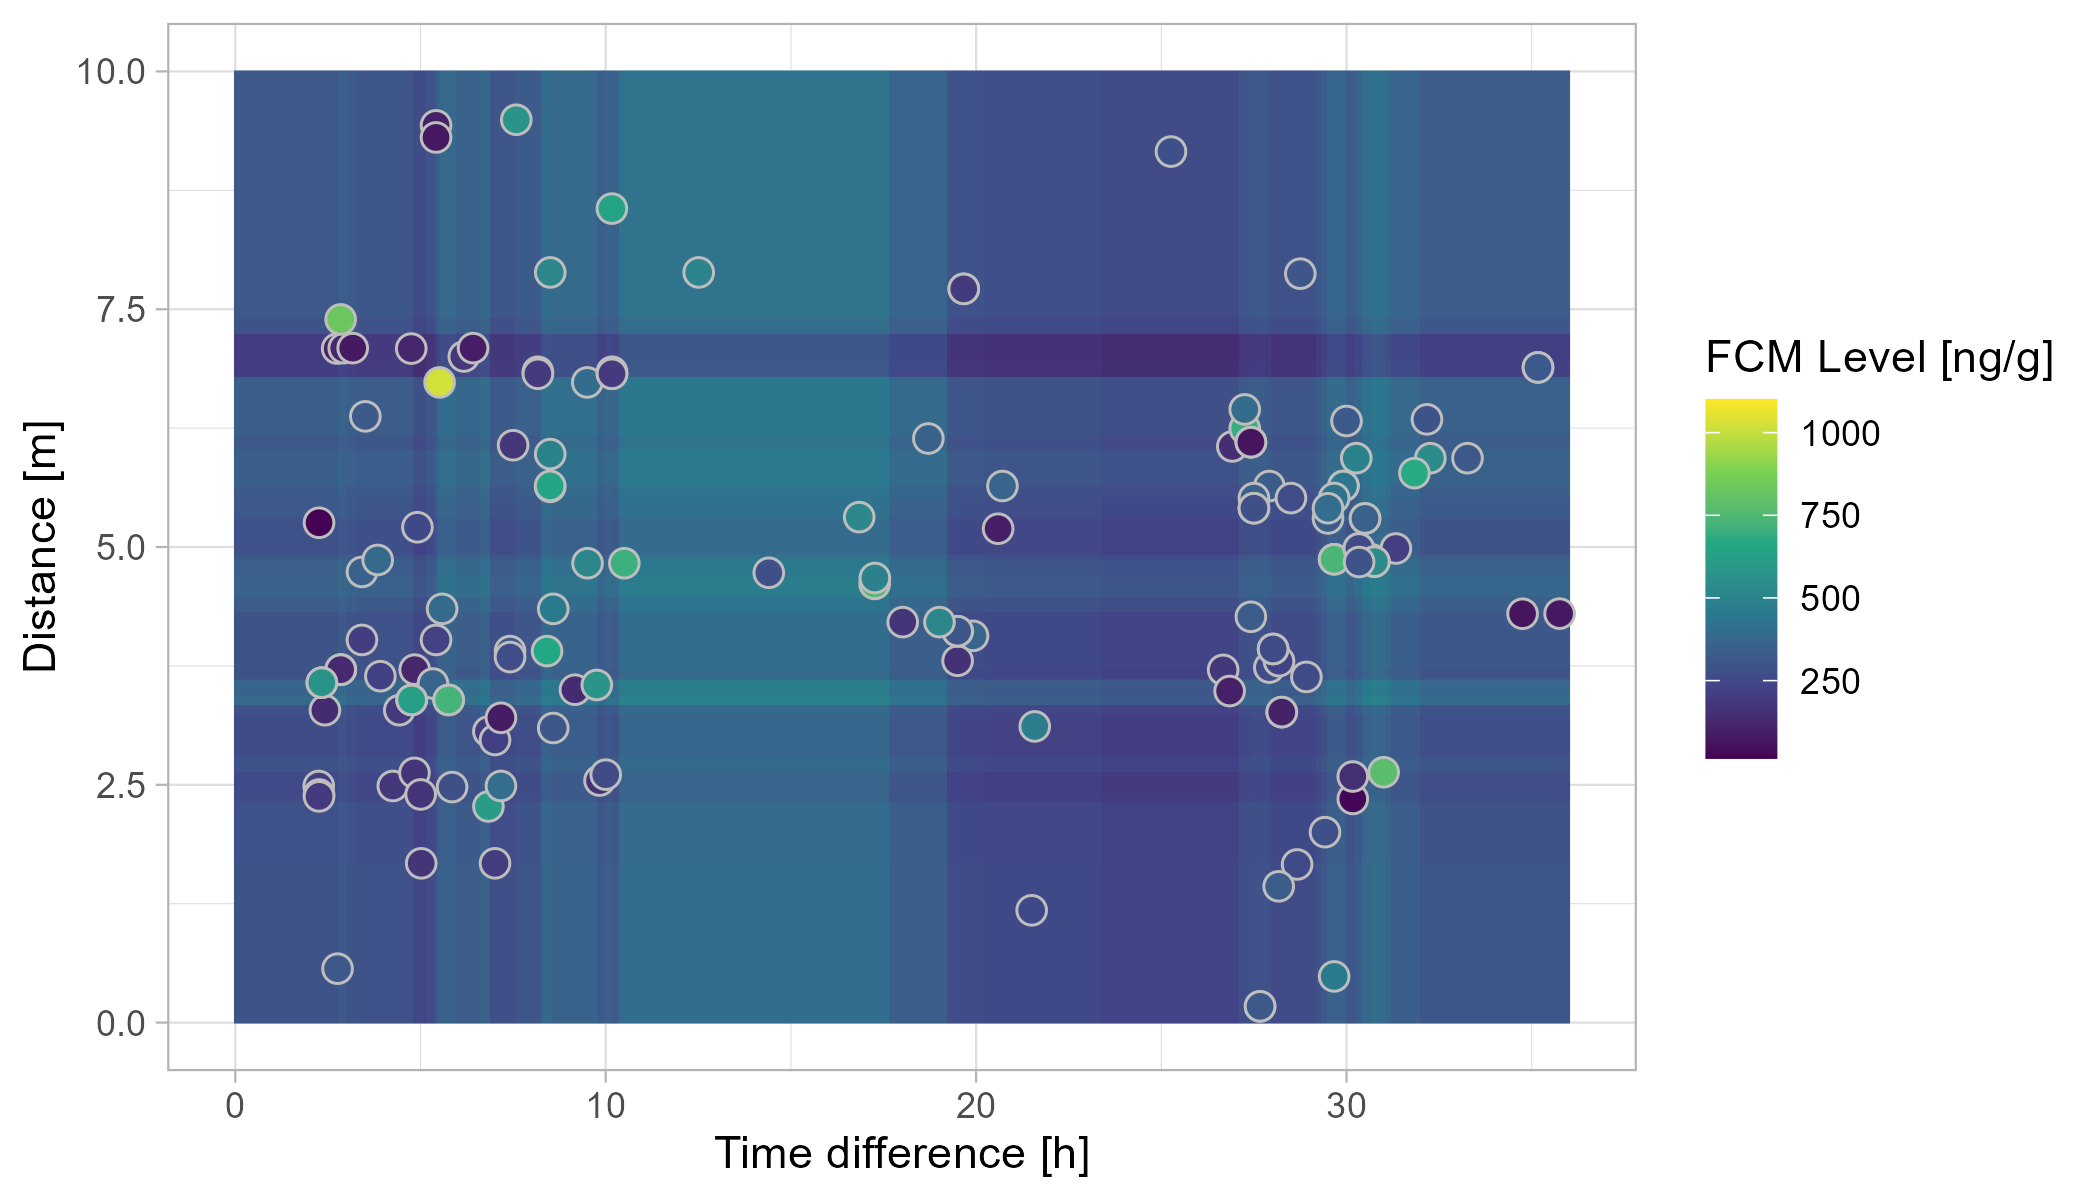
\includegraphics[keepaspectratio]{Figures/Models/xgboost_nearest.png}}

\subcaption{\label{}Nearest}
\end{minipage}%
\newline
\begin{minipage}{\linewidth}

\pandocbounded{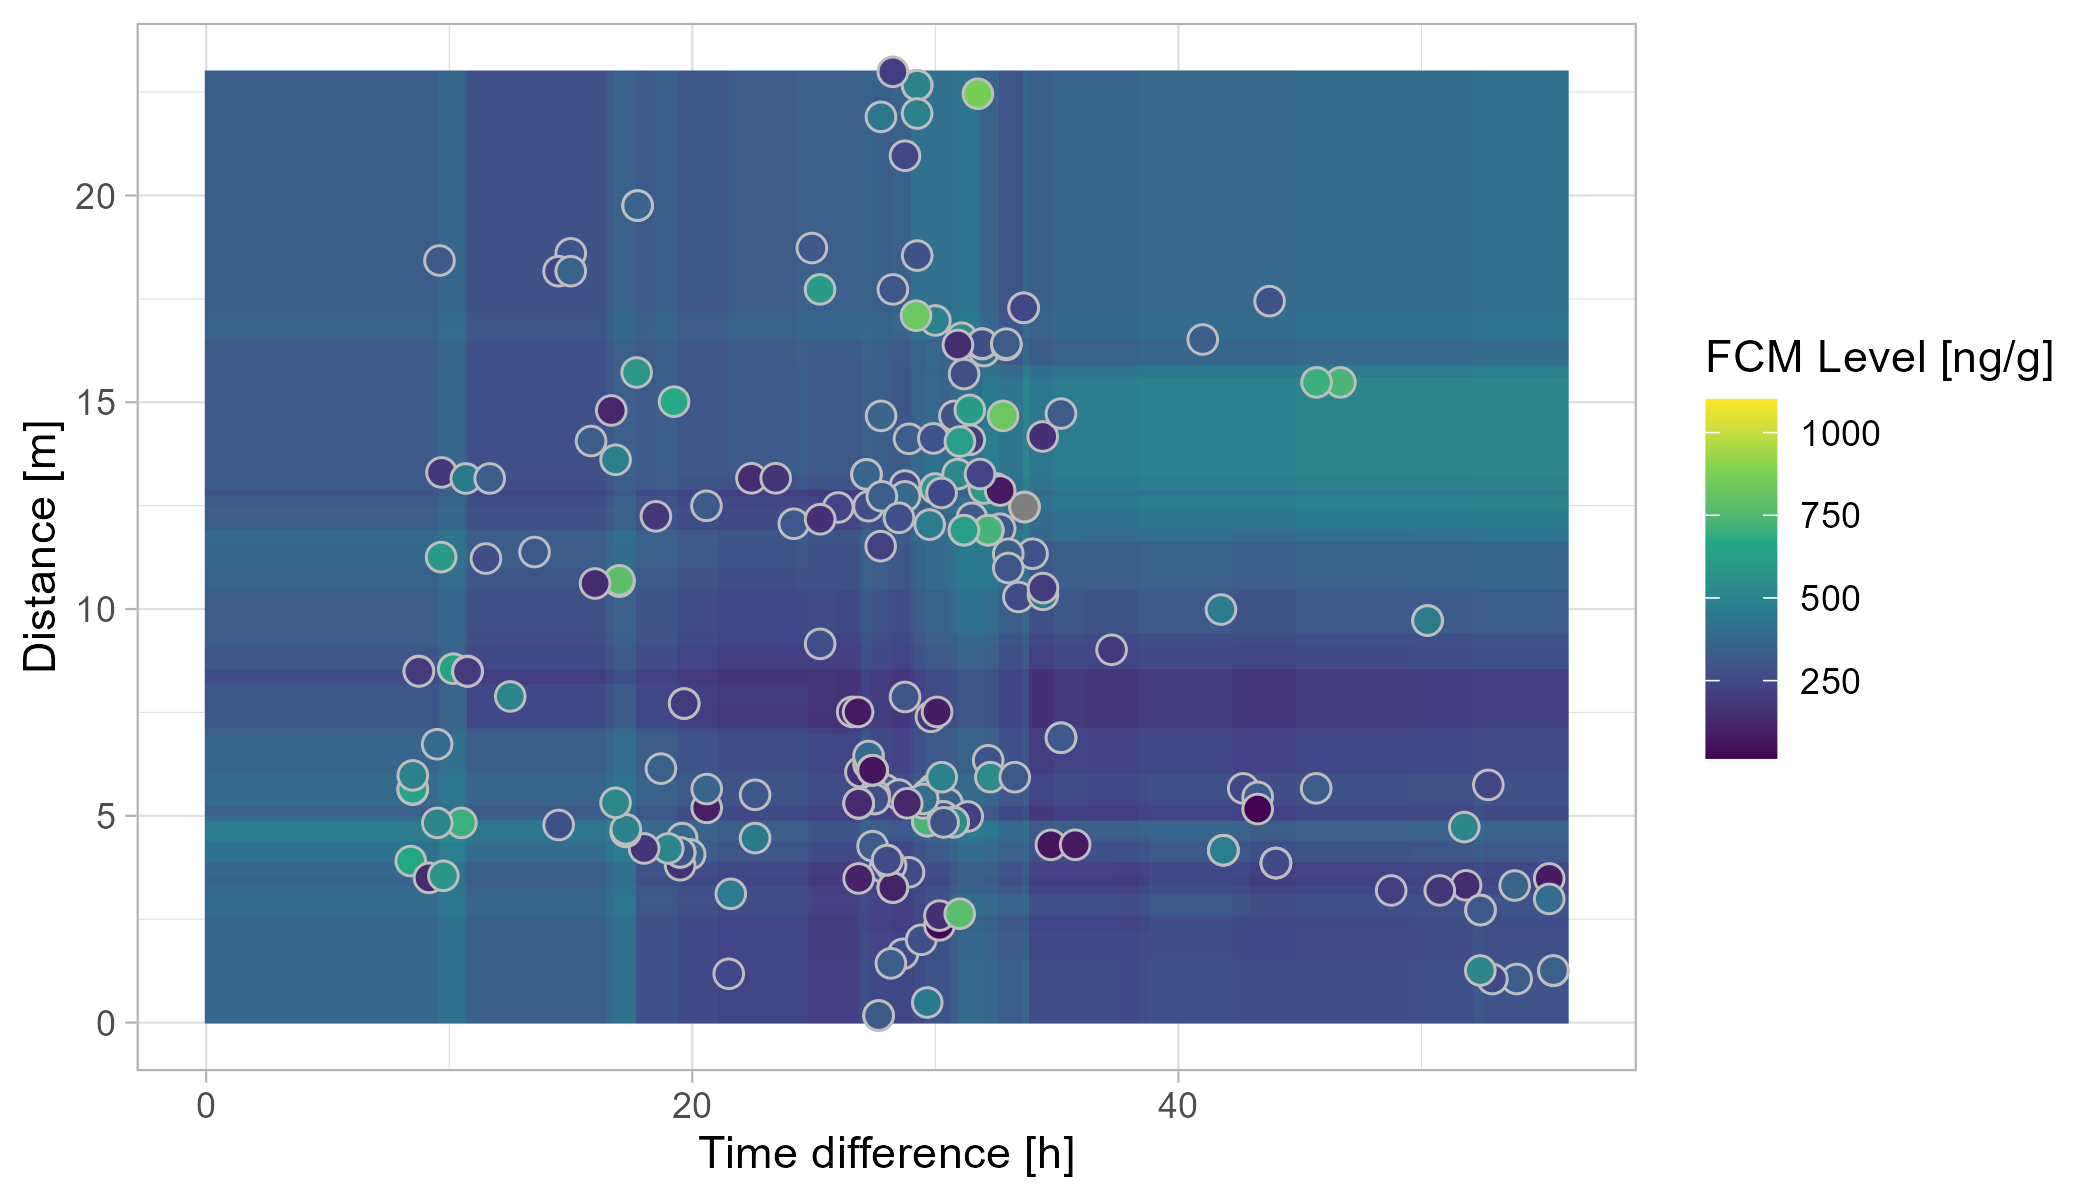
\includegraphics[keepaspectratio]{Figures/Models/xgboost_score.png}}

\subcaption{\label{}Highest score}
\end{minipage}%

\caption{\label{fig-xgboost_predictions}Predictions of XGBoost models on
the three datasets. The points are all observations within each
dataset.}

\end{figure}%

We visualize the predictions of XGBoost models in
Figure~\ref{fig-xgboost_predictions}. One would expect an increase in
the FCM level closer to the zero point, however we did not observe this
for models trained on the first two datasets. On the ``highest score''
dataset we observe a slight increase close to zero, but the same model
also predicts a high plateau for time differences above 33 hours and
spatial distances between 11.5 and 16 km. The XGBoost models show a
relatively weak and very unclear effect.

\chapter{Conclusion \& Outlook}\label{sec-outlook}

Due to the high level of uncertainty in the data, we were not able to
show a consistent effect of spatial and temporal proximity to a hunting
event on the FCM levels. However, we were able to show to a certain
extent that the FCM level decreases with increasing sample delay.

We believe that a more rigorous approach to recording hunting events
(e.g., tracking timespans rather than single moments and enforcing
complete timestamps), coupled with a larger dataset and a more directed
strategy (e.g., intentionally creating greater overlap of hunting
events, movement data, and fecal samples in time and space), could
reduce uncertainty and yield clearer results.

\chapter*{Acknowledgements}
\addcontentsline{toc}{chapter}{Acknowledgements}

We would like to express our deepest gratitude to \emph{Dr.~Nicolas
Ferry} for providing us with the opportunity to work on this project.

\emph{Daniel Schlichting}'s mentorship throughout the project was
invaluable. We thank him for his guidance and patience.

\chapter*{References}
\addcontentsline{toc}{chapter}{References}

\phantomsection\label{refs}
\begin{CSLReferences}{1}{0}
\bibitem[\citeproctext]{ref-Bergstra2012}
Bergstra, James, and Yoshua Bengio. 2012. {``Random Search for
Hyper-Parameter Optimization.''} \emph{J. Mach. Learn. Res.} 13 (null):
281--305.

\bibitem[\citeproctext]{ref-Chen2016}
Chen, Tianqi, and Carlos Guestrin. 2016. {``XGBoost: A Scalable Tree
Boosting System.''} In \emph{Proceedings of the 22nd ACM SIGKDD
International Conference on Knowledge Discovery and Data Mining},
785--94. KDD '16. New York, NY, USA: Association for Computing
Machinery. \url{https://doi.org/10.1145/2939672.2939785}.

\bibitem[\citeproctext]{ref-ChenXgboost}
Chen, Tianqi, Tong He, Michael Benesty, Vadim Khotilovich, Yuan Tang,
Hyunsu Cho, Kailong Chen, et al. 2024. {``Xgboost: {Extreme Gradient
Boosting}.''}

\bibitem[\citeproctext]{ref-Huber2003}
Huber, Susanne, Rupert Palme, Wolfgang Zenker, and Erich Möstl. 2003.
{``Non-Invasive Monitoring of the Adrenocortical Response in Red
Deer.''} \emph{Journal of Wildlife Management} 67 (April): 258--66.
\url{https://doi.org/10.2307/3802767}.

\bibitem[\citeproctext]{ref-Pinero2025}
Piñero, Justin, Heiko Jansen, Charles Robbins, Ellery Vincent, and Diana
Lafferty. 2025. {``Blood Cortisol and Faecal Cortisol Metabolite
Concentrations Following an ACTH Challenge in Unanaesthetized Brown
Bears ( Ursus Arctos ).''} \emph{Conservation Physiology} 13 (January).
\url{https://doi.org/10.1093/conphys/coae093}.

\bibitem[\citeproctext]{ref-Vilela2020}
Vilela, Sofia, António Alves da Silva, Rupert Palme, Kathreen E.
Ruckstuhl, José Paulo Sousa, and Joana Alves. 2020. {``Physiological
{Stress Reactions} in {Red Deer Induced} by {Hunting Activities}.''}
\emph{Animals: An Open Access Journal from MDPI} 10 (6): 1003.
\url{https://doi.org/10.3390/ani10061003}.

\bibitem[\citeproctext]{ref-mgcv}
Wood, S. N. 2011. {``Fast Stable Restricted Maximum Likelihood and
Marginal Likelihood Estimation of Semiparametric Generalized Linear
Models.''} \emph{Journal of the Royal Statistical Society (B)} 73 (1):
3--36.

\end{CSLReferences}

\onecolumn

\chapter{Appendix}\label{appendix}

\section{Reproduction data}\label{sec-feature_selection}

As the reproductive data only contain information on a subset of the
deer, we were faced with the decision of how to label the rest of the
deer (``pregnant''/``not pregnant''/NA). We are convinced that imputing
this information would introduce a huge bias. For this reason, we
deliberately chose not to include pregnancy data in our model. However,
we are strongly in favour of including additional characteristics that
could explain a shift in baseline stress levels.

\section{GAMM}\label{gamm}

\begin{figure}

\begin{minipage}{0.50\linewidth}

\pandocbounded{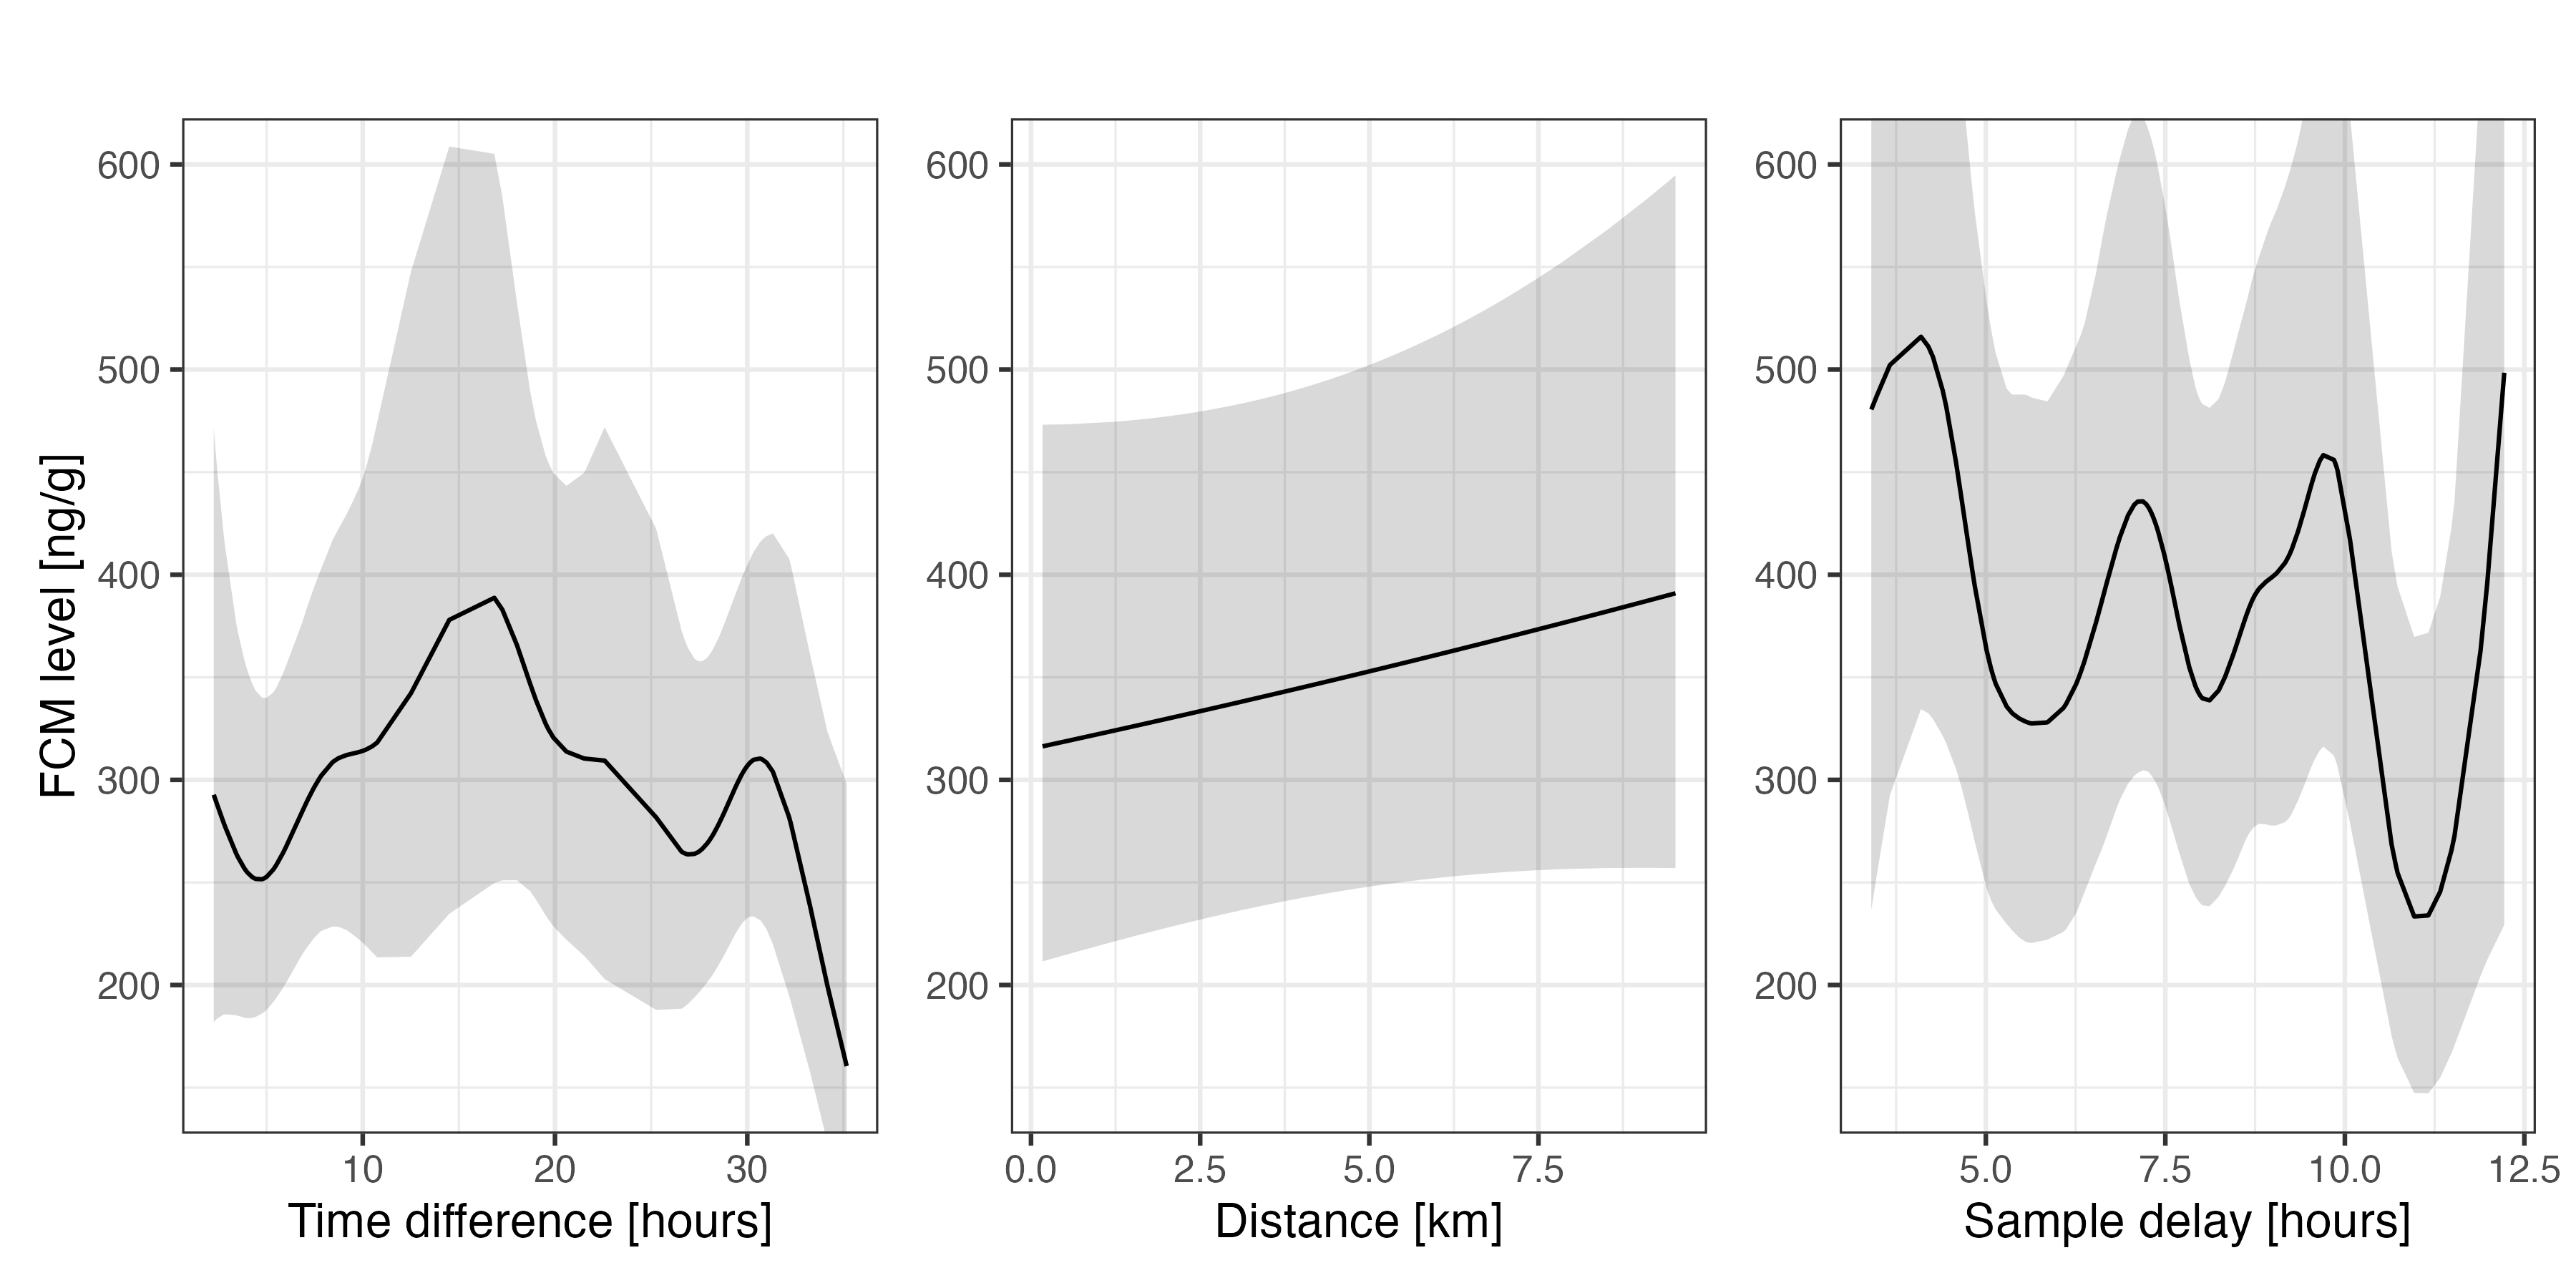
\includegraphics[keepaspectratio]{Figures/Models/last_GCV.Cp_diagnostic_custom.png}}

\subcaption{\label{}Closest in time.}
\end{minipage}%
%
\begin{minipage}{0.50\linewidth}

\pandocbounded{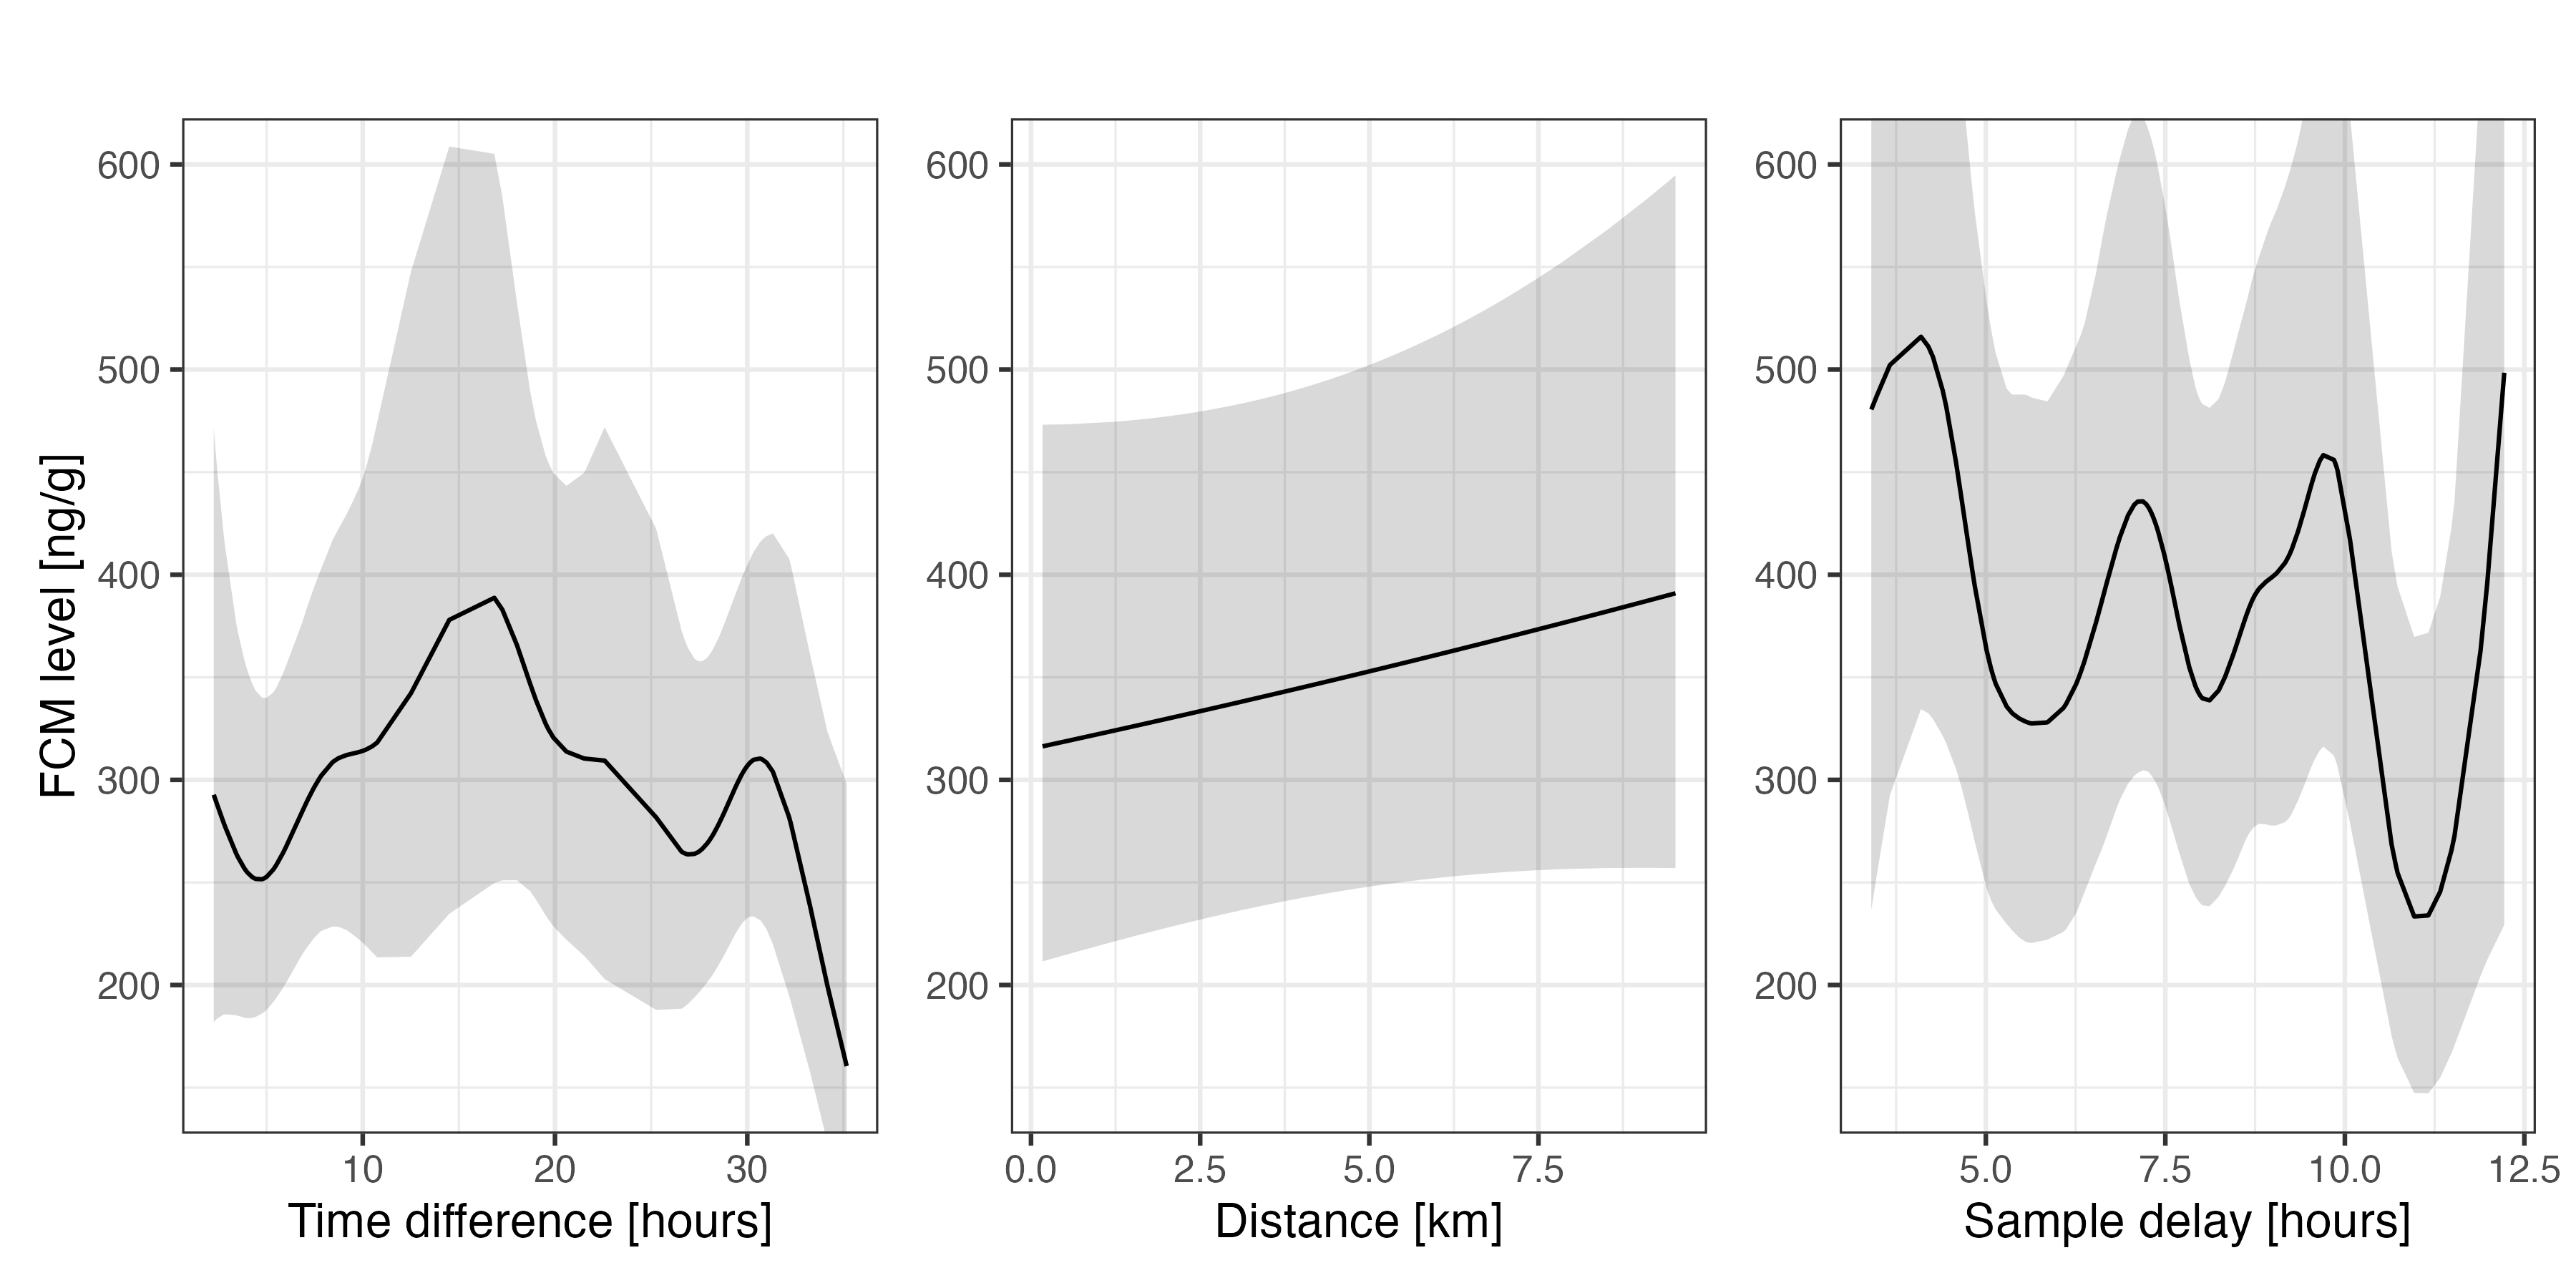
\includegraphics[keepaspectratio]{Figures/Models/last_GCV.Cp_diagnostic_custom.png}}

\subcaption{\label{}Nearest.}
\end{minipage}%
\newline
\begin{minipage}{0.50\linewidth}

\pandocbounded{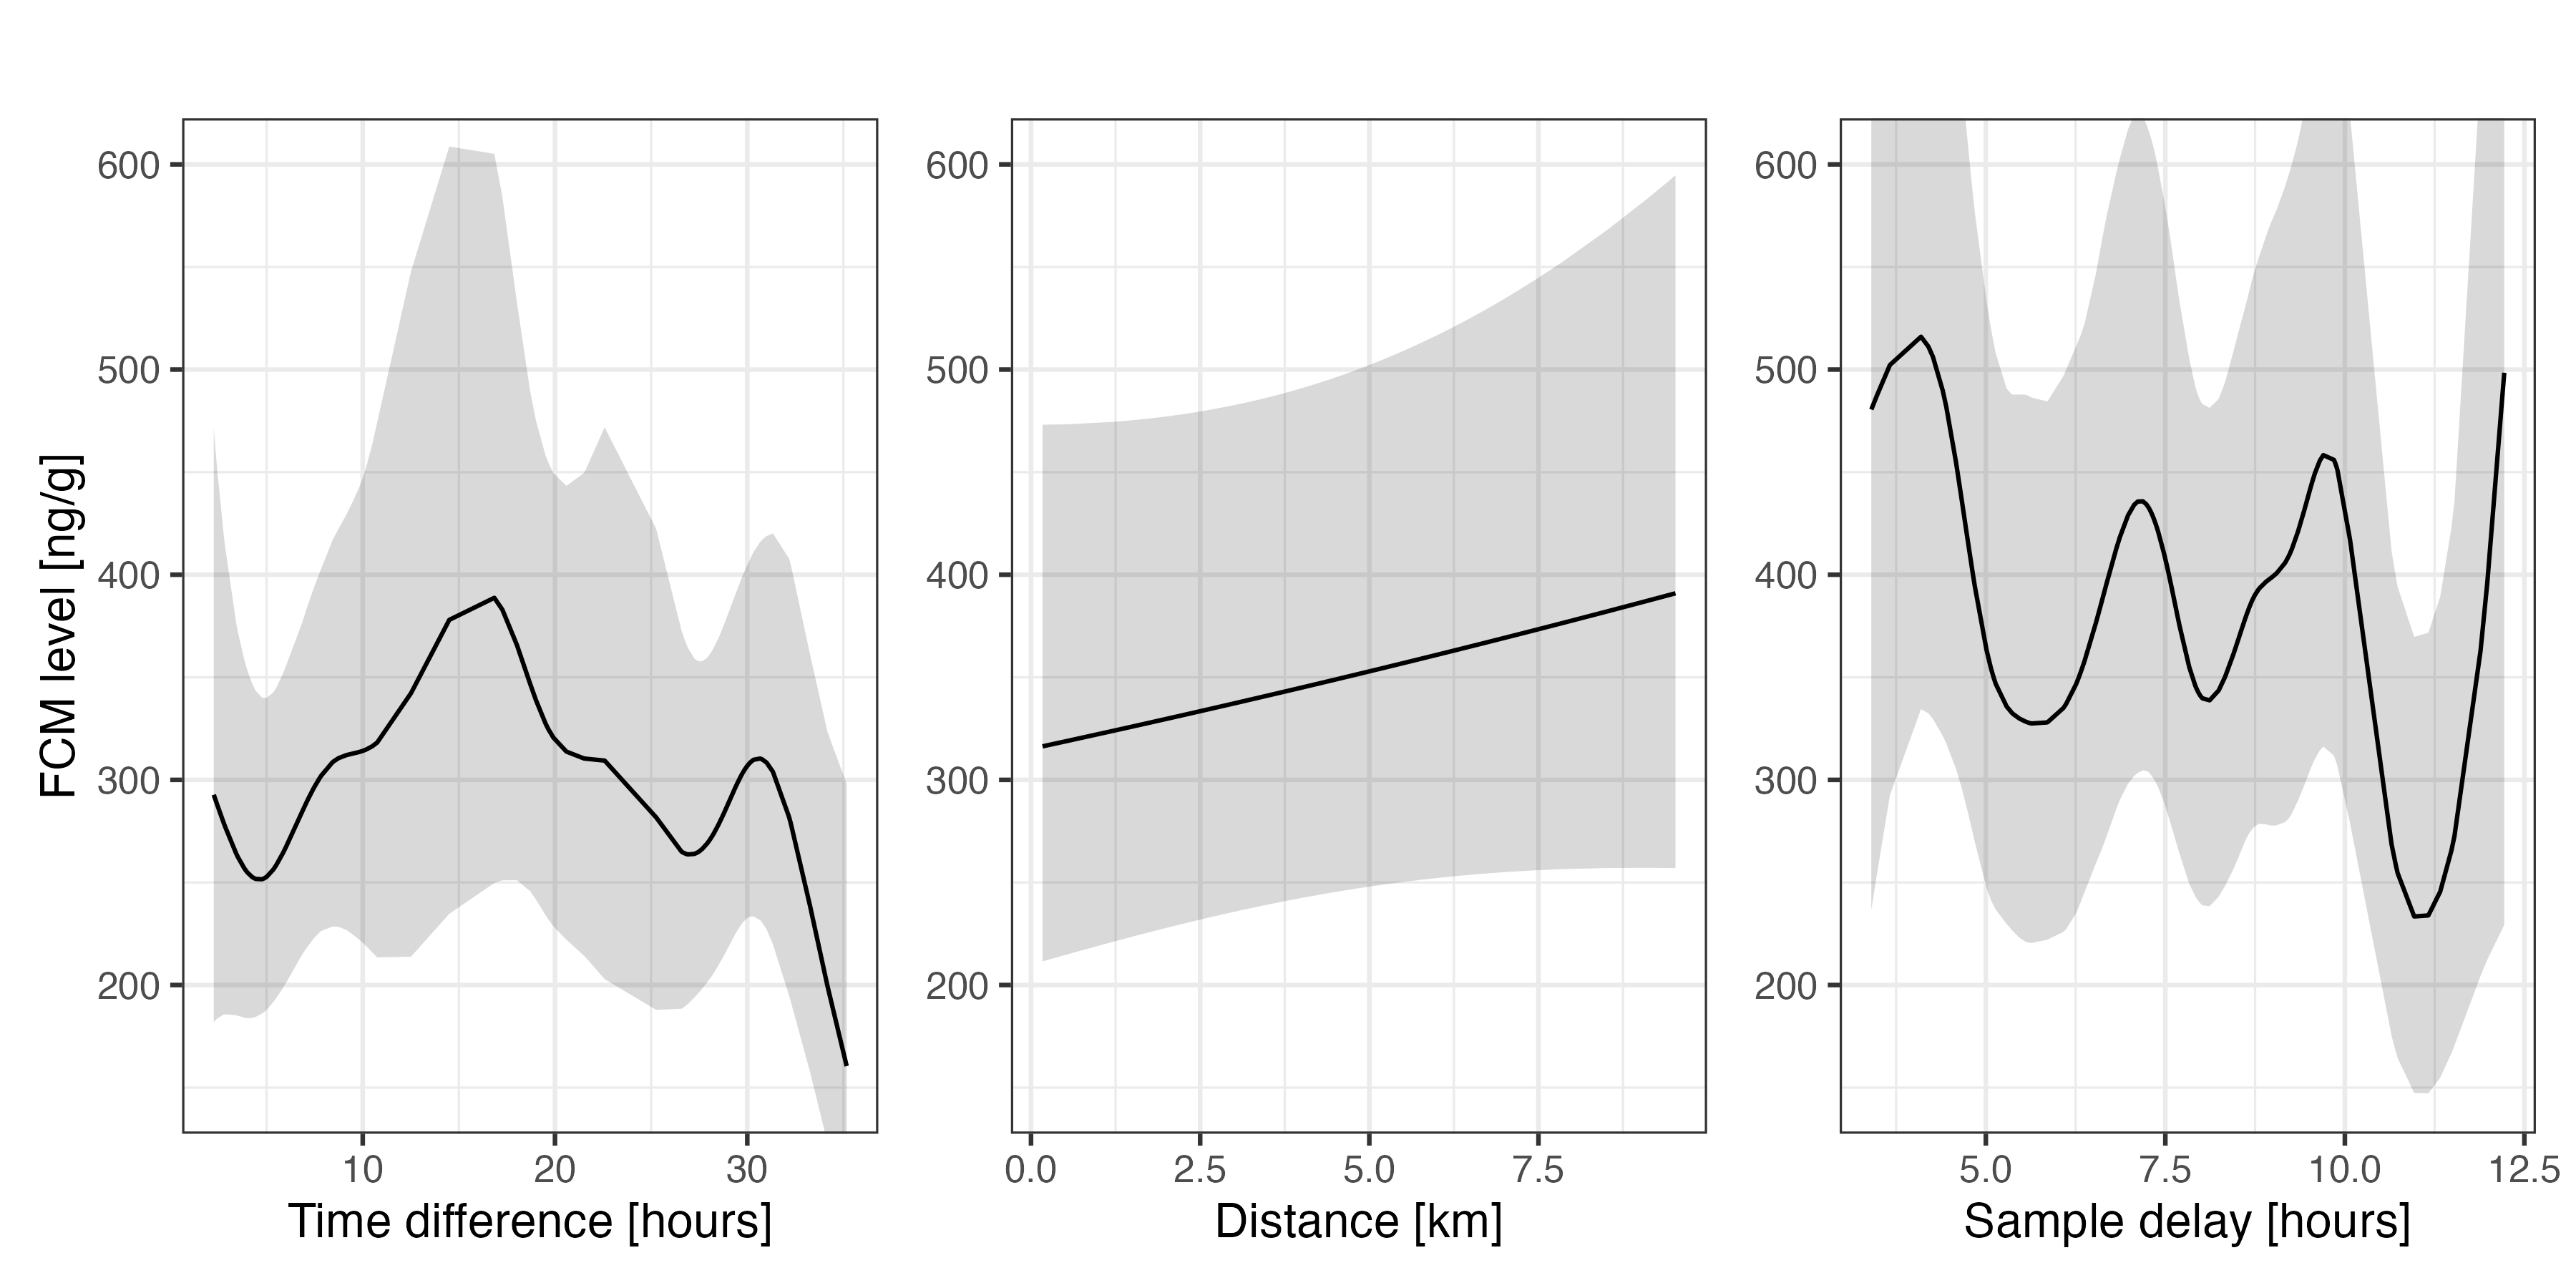
\includegraphics[keepaspectratio]{Figures/Models/last_GCV.Cp_diagnostic_custom.png}}

\subcaption{\label{}Highest score.}
\end{minipage}%

\caption{\label{fig-gamm-gcv}Adjusted predictions for the FCM level on
the three datasets. Here the GAMM is fitted using the GCV method.}

\end{figure}%

\begin{figure}

\centering{

\pandocbounded{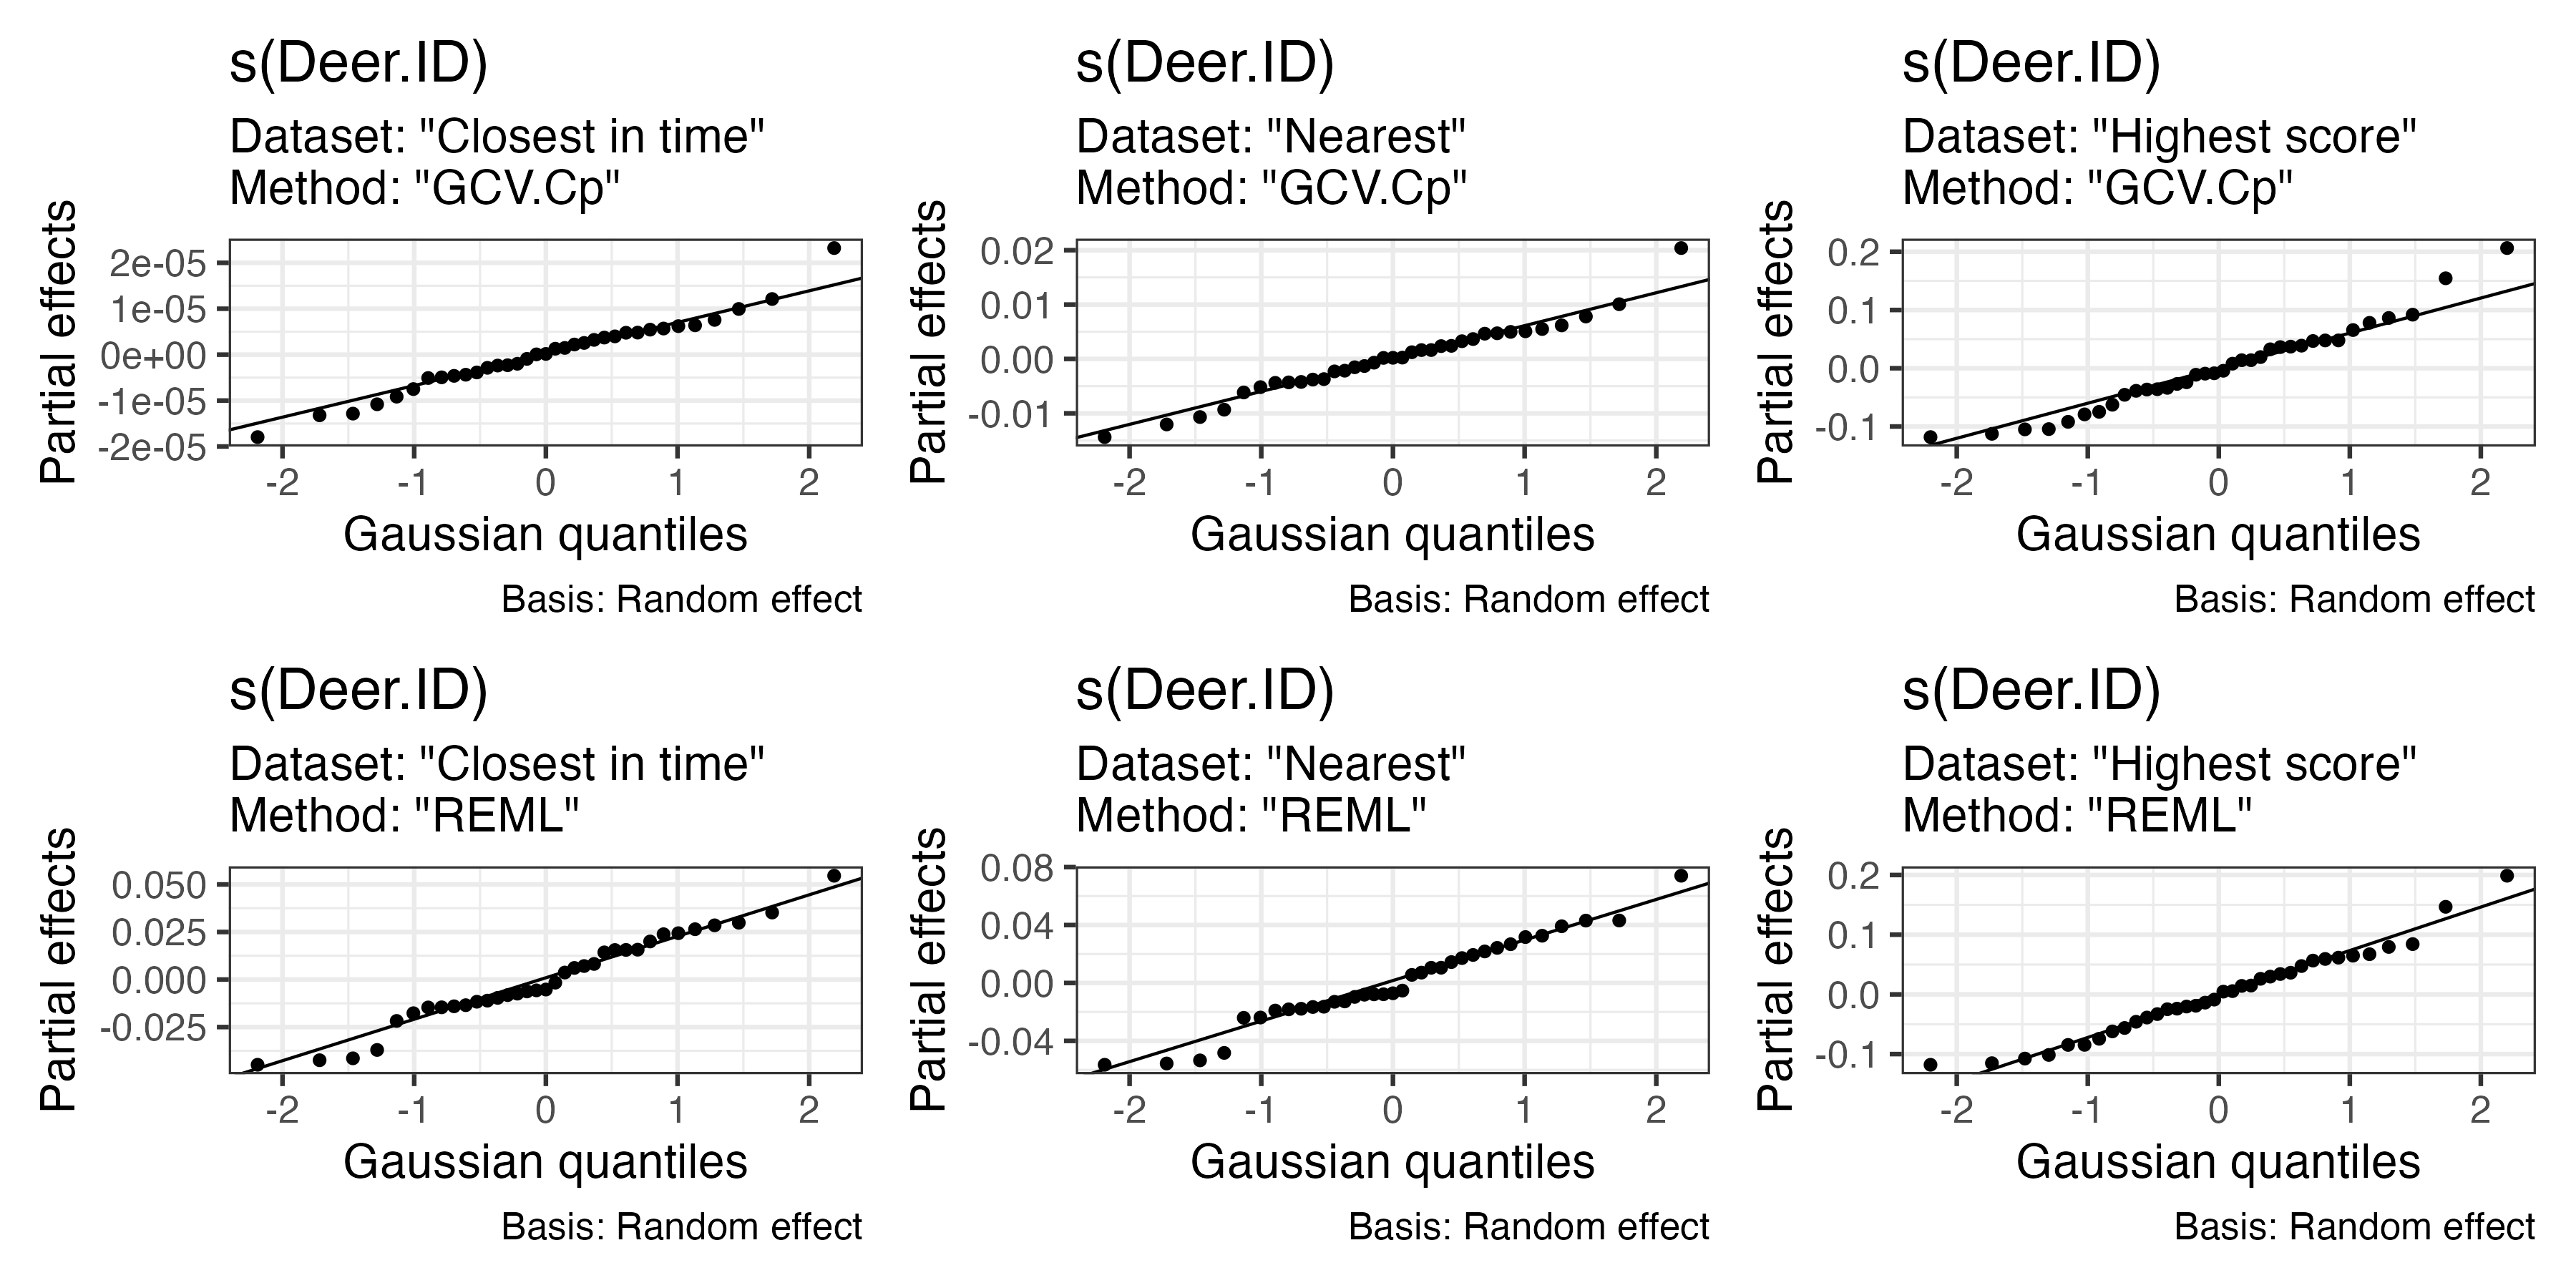
\includegraphics[keepaspectratio]{Figures/Models/partial_effect_feature_5.png}}

}

\caption{\label{fig-ri}Random intercept estimates on the three datasets
using REML and GCV.}

\end{figure}%

\newpage

\section{XGBoost}\label{xgboost-1}

\begin{figure}[H]

{\centering \pandocbounded{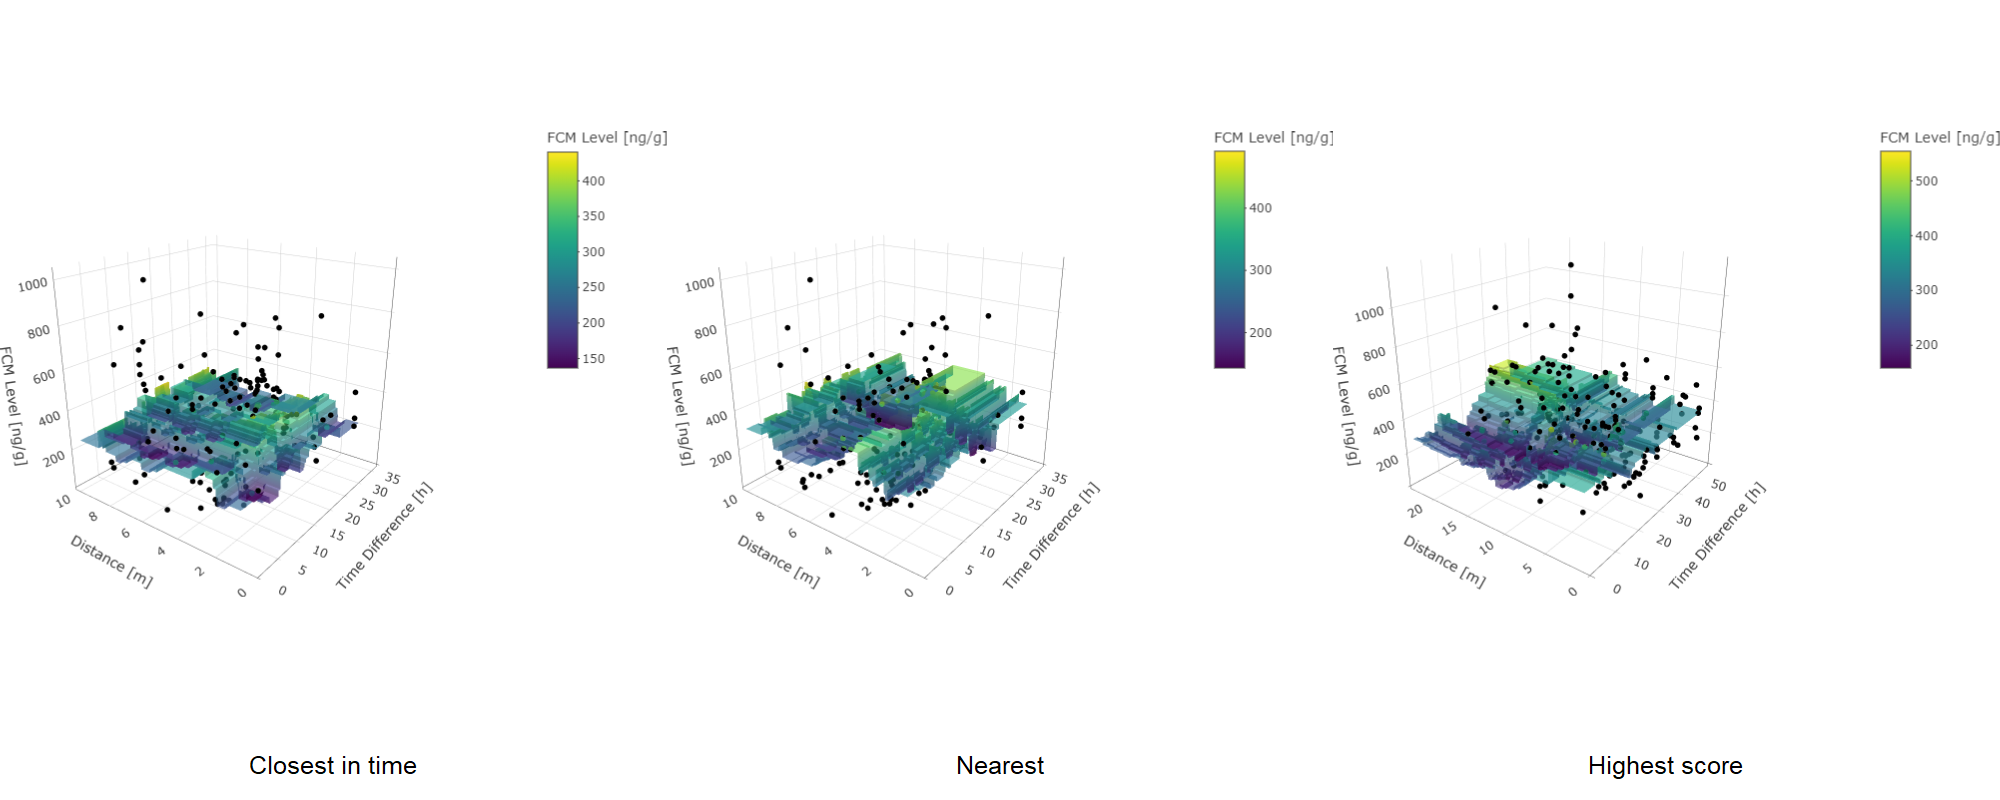
\includegraphics[keepaspectratio]{Figures/Models/combined_xgboost_plots.png}}

}

\caption{3D Visualization of predictions for the FCM level on the three
datasets by the XGBoost models. The observed data are shown as black
points.}

\end{figure}%

\begin{table}

\caption{\label{tbl-xgboost_hp}Tuned hyperparameters for the XGBoost
models.}

\centering{

\centering\begingroup\fontsize{10}{12}\selectfont

\begin{tabular}{rrrrrrr}
\toprule
DataSet & Max. depth & $\eta$ & $\gamma$ & Subsample & Features by tree & Min. weight of child\\
\midrule
Closest in time & 4 & 0.16 & 5.85 & 0.59 & 0.99 & 4.64\\
Nearest & 4 & 0.17 & 5.89 & 0.60 & 0.98 & 4.75\\
Score & 5 & 0.17 & 5.83 & 0.61 & 1.00 & 4.77\\
\bottomrule
\end{tabular}
\endgroup{}

}

\end{table}%




\end{document}
